% Generated by Sphinx.
\def\sphinxdocclass{report}
\documentclass[letterpaper,10pt,openany,oneside]{sphinxmanual}
\usepackage[utf8]{inputenc}
\DeclareUnicodeCharacter{00A0}{\nobreakspace}
\usepackage[T1]{fontenc}
\usepackage[english]{babel}
\usepackage{times}
\usepackage[Bjarne]{fncychap}
\usepackage{longtable}
\usepackage{sphinx}
\usepackage{multirow}


\title{Parallel Patternlets}
\date{March 07, 2014}
\release{}
\author{CSinParallel Project}
\newcommand{\sphinxlogo}{}
\renewcommand{\releasename}{}
\makeindex

\makeatletter
\def\PYG@reset{\let\PYG@it=\relax \let\PYG@bf=\relax%
    \let\PYG@ul=\relax \let\PYG@tc=\relax%
    \let\PYG@bc=\relax \let\PYG@ff=\relax}
\def\PYG@tok#1{\csname PYG@tok@#1\endcsname}
\def\PYG@toks#1+{\ifx\relax#1\empty\else%
    \PYG@tok{#1}\expandafter\PYG@toks\fi}
\def\PYG@do#1{\PYG@bc{\PYG@tc{\PYG@ul{%
    \PYG@it{\PYG@bf{\PYG@ff{#1}}}}}}}
\def\PYG#1#2{\PYG@reset\PYG@toks#1+\relax+\PYG@do{#2}}

\expandafter\def\csname PYG@tok@gd\endcsname{\def\PYG@tc##1{\textcolor[rgb]{0.63,0.00,0.00}{##1}}}
\expandafter\def\csname PYG@tok@gu\endcsname{\let\PYG@bf=\textbf\def\PYG@tc##1{\textcolor[rgb]{0.50,0.00,0.50}{##1}}}
\expandafter\def\csname PYG@tok@gt\endcsname{\def\PYG@tc##1{\textcolor[rgb]{0.00,0.25,0.82}{##1}}}
\expandafter\def\csname PYG@tok@gs\endcsname{\let\PYG@bf=\textbf}
\expandafter\def\csname PYG@tok@gr\endcsname{\def\PYG@tc##1{\textcolor[rgb]{1.00,0.00,0.00}{##1}}}
\expandafter\def\csname PYG@tok@cm\endcsname{\let\PYG@it=\textit\def\PYG@tc##1{\textcolor[rgb]{0.25,0.50,0.56}{##1}}}
\expandafter\def\csname PYG@tok@vg\endcsname{\def\PYG@tc##1{\textcolor[rgb]{0.73,0.38,0.84}{##1}}}
\expandafter\def\csname PYG@tok@m\endcsname{\def\PYG@tc##1{\textcolor[rgb]{0.13,0.50,0.31}{##1}}}
\expandafter\def\csname PYG@tok@mh\endcsname{\def\PYG@tc##1{\textcolor[rgb]{0.13,0.50,0.31}{##1}}}
\expandafter\def\csname PYG@tok@cs\endcsname{\def\PYG@tc##1{\textcolor[rgb]{0.25,0.50,0.56}{##1}}\def\PYG@bc##1{\setlength{\fboxsep}{0pt}\colorbox[rgb]{1.00,0.94,0.94}{\strut ##1}}}
\expandafter\def\csname PYG@tok@ge\endcsname{\let\PYG@it=\textit}
\expandafter\def\csname PYG@tok@vc\endcsname{\def\PYG@tc##1{\textcolor[rgb]{0.73,0.38,0.84}{##1}}}
\expandafter\def\csname PYG@tok@il\endcsname{\def\PYG@tc##1{\textcolor[rgb]{0.13,0.50,0.31}{##1}}}
\expandafter\def\csname PYG@tok@go\endcsname{\def\PYG@tc##1{\textcolor[rgb]{0.19,0.19,0.19}{##1}}}
\expandafter\def\csname PYG@tok@cp\endcsname{\def\PYG@tc##1{\textcolor[rgb]{0.00,0.44,0.13}{##1}}}
\expandafter\def\csname PYG@tok@gi\endcsname{\def\PYG@tc##1{\textcolor[rgb]{0.00,0.63,0.00}{##1}}}
\expandafter\def\csname PYG@tok@gh\endcsname{\let\PYG@bf=\textbf\def\PYG@tc##1{\textcolor[rgb]{0.00,0.00,0.50}{##1}}}
\expandafter\def\csname PYG@tok@ni\endcsname{\let\PYG@bf=\textbf\def\PYG@tc##1{\textcolor[rgb]{0.84,0.33,0.22}{##1}}}
\expandafter\def\csname PYG@tok@nl\endcsname{\let\PYG@bf=\textbf\def\PYG@tc##1{\textcolor[rgb]{0.00,0.13,0.44}{##1}}}
\expandafter\def\csname PYG@tok@nn\endcsname{\let\PYG@bf=\textbf\def\PYG@tc##1{\textcolor[rgb]{0.05,0.52,0.71}{##1}}}
\expandafter\def\csname PYG@tok@no\endcsname{\def\PYG@tc##1{\textcolor[rgb]{0.38,0.68,0.84}{##1}}}
\expandafter\def\csname PYG@tok@na\endcsname{\def\PYG@tc##1{\textcolor[rgb]{0.25,0.44,0.63}{##1}}}
\expandafter\def\csname PYG@tok@nb\endcsname{\def\PYG@tc##1{\textcolor[rgb]{0.00,0.44,0.13}{##1}}}
\expandafter\def\csname PYG@tok@nc\endcsname{\let\PYG@bf=\textbf\def\PYG@tc##1{\textcolor[rgb]{0.05,0.52,0.71}{##1}}}
\expandafter\def\csname PYG@tok@nd\endcsname{\let\PYG@bf=\textbf\def\PYG@tc##1{\textcolor[rgb]{0.33,0.33,0.33}{##1}}}
\expandafter\def\csname PYG@tok@ne\endcsname{\def\PYG@tc##1{\textcolor[rgb]{0.00,0.44,0.13}{##1}}}
\expandafter\def\csname PYG@tok@nf\endcsname{\def\PYG@tc##1{\textcolor[rgb]{0.02,0.16,0.49}{##1}}}
\expandafter\def\csname PYG@tok@si\endcsname{\let\PYG@it=\textit\def\PYG@tc##1{\textcolor[rgb]{0.44,0.63,0.82}{##1}}}
\expandafter\def\csname PYG@tok@s2\endcsname{\def\PYG@tc##1{\textcolor[rgb]{0.25,0.44,0.63}{##1}}}
\expandafter\def\csname PYG@tok@vi\endcsname{\def\PYG@tc##1{\textcolor[rgb]{0.73,0.38,0.84}{##1}}}
\expandafter\def\csname PYG@tok@nt\endcsname{\let\PYG@bf=\textbf\def\PYG@tc##1{\textcolor[rgb]{0.02,0.16,0.45}{##1}}}
\expandafter\def\csname PYG@tok@nv\endcsname{\def\PYG@tc##1{\textcolor[rgb]{0.73,0.38,0.84}{##1}}}
\expandafter\def\csname PYG@tok@s1\endcsname{\def\PYG@tc##1{\textcolor[rgb]{0.25,0.44,0.63}{##1}}}
\expandafter\def\csname PYG@tok@gp\endcsname{\let\PYG@bf=\textbf\def\PYG@tc##1{\textcolor[rgb]{0.78,0.36,0.04}{##1}}}
\expandafter\def\csname PYG@tok@sh\endcsname{\def\PYG@tc##1{\textcolor[rgb]{0.25,0.44,0.63}{##1}}}
\expandafter\def\csname PYG@tok@ow\endcsname{\let\PYG@bf=\textbf\def\PYG@tc##1{\textcolor[rgb]{0.00,0.44,0.13}{##1}}}
\expandafter\def\csname PYG@tok@sx\endcsname{\def\PYG@tc##1{\textcolor[rgb]{0.78,0.36,0.04}{##1}}}
\expandafter\def\csname PYG@tok@bp\endcsname{\def\PYG@tc##1{\textcolor[rgb]{0.00,0.44,0.13}{##1}}}
\expandafter\def\csname PYG@tok@c1\endcsname{\let\PYG@it=\textit\def\PYG@tc##1{\textcolor[rgb]{0.25,0.50,0.56}{##1}}}
\expandafter\def\csname PYG@tok@kc\endcsname{\let\PYG@bf=\textbf\def\PYG@tc##1{\textcolor[rgb]{0.00,0.44,0.13}{##1}}}
\expandafter\def\csname PYG@tok@c\endcsname{\let\PYG@it=\textit\def\PYG@tc##1{\textcolor[rgb]{0.25,0.50,0.56}{##1}}}
\expandafter\def\csname PYG@tok@mf\endcsname{\def\PYG@tc##1{\textcolor[rgb]{0.13,0.50,0.31}{##1}}}
\expandafter\def\csname PYG@tok@err\endcsname{\def\PYG@bc##1{\setlength{\fboxsep}{0pt}\fcolorbox[rgb]{1.00,0.00,0.00}{1,1,1}{\strut ##1}}}
\expandafter\def\csname PYG@tok@kd\endcsname{\let\PYG@bf=\textbf\def\PYG@tc##1{\textcolor[rgb]{0.00,0.44,0.13}{##1}}}
\expandafter\def\csname PYG@tok@ss\endcsname{\def\PYG@tc##1{\textcolor[rgb]{0.32,0.47,0.09}{##1}}}
\expandafter\def\csname PYG@tok@sr\endcsname{\def\PYG@tc##1{\textcolor[rgb]{0.14,0.33,0.53}{##1}}}
\expandafter\def\csname PYG@tok@mo\endcsname{\def\PYG@tc##1{\textcolor[rgb]{0.13,0.50,0.31}{##1}}}
\expandafter\def\csname PYG@tok@mi\endcsname{\def\PYG@tc##1{\textcolor[rgb]{0.13,0.50,0.31}{##1}}}
\expandafter\def\csname PYG@tok@kn\endcsname{\let\PYG@bf=\textbf\def\PYG@tc##1{\textcolor[rgb]{0.00,0.44,0.13}{##1}}}
\expandafter\def\csname PYG@tok@o\endcsname{\def\PYG@tc##1{\textcolor[rgb]{0.40,0.40,0.40}{##1}}}
\expandafter\def\csname PYG@tok@kr\endcsname{\let\PYG@bf=\textbf\def\PYG@tc##1{\textcolor[rgb]{0.00,0.44,0.13}{##1}}}
\expandafter\def\csname PYG@tok@s\endcsname{\def\PYG@tc##1{\textcolor[rgb]{0.25,0.44,0.63}{##1}}}
\expandafter\def\csname PYG@tok@kp\endcsname{\def\PYG@tc##1{\textcolor[rgb]{0.00,0.44,0.13}{##1}}}
\expandafter\def\csname PYG@tok@w\endcsname{\def\PYG@tc##1{\textcolor[rgb]{0.73,0.73,0.73}{##1}}}
\expandafter\def\csname PYG@tok@kt\endcsname{\def\PYG@tc##1{\textcolor[rgb]{0.56,0.13,0.00}{##1}}}
\expandafter\def\csname PYG@tok@sc\endcsname{\def\PYG@tc##1{\textcolor[rgb]{0.25,0.44,0.63}{##1}}}
\expandafter\def\csname PYG@tok@sb\endcsname{\def\PYG@tc##1{\textcolor[rgb]{0.25,0.44,0.63}{##1}}}
\expandafter\def\csname PYG@tok@k\endcsname{\let\PYG@bf=\textbf\def\PYG@tc##1{\textcolor[rgb]{0.00,0.44,0.13}{##1}}}
\expandafter\def\csname PYG@tok@se\endcsname{\let\PYG@bf=\textbf\def\PYG@tc##1{\textcolor[rgb]{0.25,0.44,0.63}{##1}}}
\expandafter\def\csname PYG@tok@sd\endcsname{\let\PYG@it=\textit\def\PYG@tc##1{\textcolor[rgb]{0.25,0.44,0.63}{##1}}}

\def\PYGZbs{\char`\\}
\def\PYGZus{\char`\_}
\def\PYGZob{\char`\{}
\def\PYGZcb{\char`\}}
\def\PYGZca{\char`\^}
\def\PYGZam{\char`\&}
\def\PYGZlt{\char`\<}
\def\PYGZgt{\char`\>}
\def\PYGZsh{\char`\#}
\def\PYGZpc{\char`\%}
\def\PYGZdl{\char`\$}
\def\PYGZti{\char`\~}
% for compatibility with earlier versions
\def\PYGZat{@}
\def\PYGZlb{[}
\def\PYGZrb{]}
\makeatother

\begin{document}

\maketitle
\tableofcontents
\phantomsection\label{index::doc}


This document contains simple examples of basic elements that are combined to form patterns often used in programs employing parallelism.  We call these examples \emph{patternlets} because they are deliberately trivial, small, yet functioning programs that illustrate a basic shell of how a particular parallel pattern is created in a program.  They are starting points you can use to create realistic working programs of your own that use the patterns.  Before diving into the examples, first there will be some background on parallel programming patterns.


\chapter{Parallel Programming Patterns}
\label{PatternsIntro:parallel-programming-patterns}\label{PatternsIntro::doc}\label{PatternsIntro:parallel-patternlets}
Like all programs, parallel programs contain many \textbf{patterns}: useful ways of writing code that are used repeatedly by most developers because they work well in practice.  These patterns have been documented by developers over time so that useful ways of organizing and writing good parallel code can be learned by new programmers (and even seasoned veterans).


\section{An organization of parallel patterns}
\label{PatternsIntro:an-organization-of-parallel-patterns}
When writing parallel programs, developers use patterns that can be grouped into two main categories:
\begin{enumerate}
\item {} 
Strategies

\item {} 
Concurrent Execution Mechanisms

\end{enumerate}


\subsection{Strategies}
\label{PatternsIntro:strategies}
When you set out to write a program, whether it is parallel or not, you should be considering two primary strategic considerations:
\begin{enumerate}
\item {} 
What \emph{algorithmic strategies} to use

\item {} 
Given the algorithmic strategies, what \emph{implementation strategies} to use

\end{enumerate}

In the examples in this document we introduce some well-used patterns for both algorithmic strategies and implementation strategies.  Parallel algorithmic strategies primarily have to do with making choices about what tasks can be done concurrently by multiple processing units executing concurrently.  Parallel programs often make use of several patterns of implementation strategies.  Some of these patterns contribute to the overall structure of the program, and others are concerned with how the data that is being computed by multiple processing units is structured.  As you will see, the patternlets introduce more algorithmic strategy patterns and program structure implementation strategy patterns than data structure implementation strategy patterns.


\subsection{Concurrent Execution Mechanisms}
\label{PatternsIntro:concurrent-execution-mechanisms}
There are a number of parallel code patterns that are closely related to the system or hardware that a program is being written for and the software library used to enable parallelism, or concurrent execution.  These \emph{concurrent execution} patterns fall into two major categories:
\begin{enumerate}
\item {} 
\emph{Process/Thread control} patterns, which dictate how the processing units of parallel execution on the hardware (either a process or a thread, depending on the hardware and software used) are controlled at run time.  For the patternlets described in this document, the software libraries that provide system parallelism have these patterns built into them, so they will be hidden from the programmer.

\item {} 
\emph{Coordination} patterns, which set up how multiple concurrently running tasks on processing units coordinate to complete the parallel computation desired.

\end{enumerate}

In parallel processing, most software uses one of
two major \emph{coordination patterns}:
\begin{enumerate}
\item {} 
\textbf{message passing} between concurrent processes on either single multiprocessor machines or clusters of distributed computers, and

\item {} 
\textbf{mutual exclusion} between threads executing concurrently on a single shared memory system.

\end{enumerate}

These two types of computation are often realized using two very popular C/C++ libraries:
\begin{enumerate}
\item {} 
MPI, or Message Passing Interface, for message passing.

\item {} 
OpenMP for threaded, shared memory applications.

\end{enumerate}

OpenMP is built on a lower-level POSIX library called Pthreads, which can also be used by itself on shared memory systems.

A third emerging type of parallel implementation involves a \emph{hybrid computation} that uses both of the above patterns together, using a cluster of computers, each of which executes multiple threads.  This type of hybrid program often uses MPI and OpenMP together in one program, which runs on multiple computers in a cluster.

This document is split into chapters of examples.  There are examples for message passing using MPI and shared memory using OpenMP.
(In the future we will include shared memory examples using Pthreads, and hybrid computations using a combination of MPI and OpenMP.)

Most of the examples are illustrated
with the C programming language, using standard popular available libraries. In a few cases, C++
is used to illustrate a particular difference in code execution between the two languages.

There are many small examples that serve to illustrate a common pattern.  They are designed for you to try compiling and running on your own to see how they work.  For each example, there are comments within the code to guide you as you try them out.  In some cases, there may be code snippets that you can comment and/or uncomment to see how the execution of the code changes after you do so and re-compile it.

Depending on you interest, you can now explore MPI Patternlets or OpenMP Patternlets.

{\hyperref[MessagePassing/MPI_Patternlets::doc]{\emph{Message Passing Parallel Patternlets}}}

{\hyperref[SharedMemory/OpenMP_Patternlets::doc]{\emph{Shared Memory Parallel Patternlets in OpenMP}}}


\chapter{Message Passing Parallel Patternlets}
\label{MessagePassing/MPI_Patternlets:message-passing-parallel-patternlets}\label{MessagePassing/MPI_Patternlets::doc}
Parallel programs contain \emph{patterns}:  code that recurs over and over again
in solutions to many problems.  The following examples show very simple
examples of small portions of
these patterns that can be combined to solve a problem.  These C code examples use the
Message Passing Interface (MPI) library, which is suitable for use on either a
single pultiprocessor machine or a cluster
of machines.


\section{Source Code}
\label{MessagePassing/MPI_Patternlets:source-code}
Please download all examples from this tarball:
\code{MPI.tgz}

A C code file for each example below can be found in subdirectories of the MPI directory,
along with a makefile and an example of how to execute the program.


\section{0. Single Program, Multiple Data}
\label{MessagePassing/MPI_Patternlets:single-program-multiple-data}
First let us illustrate the basic components of an MPI program,
which by its nature uses a single program that runs on each process.
Note what gets printed is different for each process, thus the
processes using this one single program can have different data values
for its variables.  This is why we call it single program, multiple data.

\begin{Verbatim}[commandchars=\\\{\}]
\PYG{c+cm}{/* spmd.c}
\PYG{c+cm}{ * ... illustrates the single program multiple data}
\PYG{c+cm}{ *      (SPMD) pattern using basic MPI commands.}
\PYG{c+cm}{ *}
\PYG{c+cm}{ * Joel Adams, Calvin College, November 2009.}
\PYG{c+cm}{ *}
\PYG{c+cm}{ * Usage: mpirun -np 4 ./spmd}
\PYG{c+cm}{ */}

\PYG{c+cp}{\PYGZsh{}}\PYG{c+cp}{include \PYGZlt{}stdio.h\PYGZgt{}}
\PYG{c+cp}{\PYGZsh{}}\PYG{c+cp}{include \PYGZlt{}mpi.h\PYGZgt{}}

\PYG{k+kt}{int} \PYG{n+nf}{main}\PYG{p}{(}\PYG{k+kt}{int} \PYG{n}{argc}\PYG{p}{,} \PYG{k+kt}{char}\PYG{o}{*}\PYG{o}{*} \PYG{n}{argv}\PYG{p}{)} \PYG{p}{\PYGZob{}}
	\PYG{k+kt}{int} \PYG{n}{id} \PYG{o}{=} \PYG{o}{-}\PYG{l+m+mi}{1}\PYG{p}{,} \PYG{n}{numProcesses} \PYG{o}{=} \PYG{o}{-}\PYG{l+m+mi}{1}\PYG{p}{,} \PYG{n}{length} \PYG{o}{=} \PYG{o}{-}\PYG{l+m+mi}{1}\PYG{p}{;}
	\PYG{k+kt}{char} \PYG{n}{myHostName}\PYG{p}{[}\PYG{n}{MPI\PYGZus{}MAX\PYGZus{}PROCESSOR\PYGZus{}NAME}\PYG{p}{]}\PYG{p}{;}

	\PYG{n}{MPI\PYGZus{}Init}\PYG{p}{(}\PYG{o}{\PYGZam{}}\PYG{n}{argc}\PYG{p}{,} \PYG{o}{\PYGZam{}}\PYG{n}{argv}\PYG{p}{)}\PYG{p}{;}
	\PYG{n}{MPI\PYGZus{}Comm\PYGZus{}rank}\PYG{p}{(}\PYG{n}{MPI\PYGZus{}COMM\PYGZus{}WORLD}\PYG{p}{,} \PYG{o}{\PYGZam{}}\PYG{n}{id}\PYG{p}{)}\PYG{p}{;}
	\PYG{n}{MPI\PYGZus{}Comm\PYGZus{}size}\PYG{p}{(}\PYG{n}{MPI\PYGZus{}COMM\PYGZus{}WORLD}\PYG{p}{,} \PYG{o}{\PYGZam{}}\PYG{n}{numProcesses}\PYG{p}{)}\PYG{p}{;}
	\PYG{n}{MPI\PYGZus{}Get\PYGZus{}processor\PYGZus{}name} \PYG{p}{(}\PYG{n}{myHostName}\PYG{p}{,} \PYG{o}{\PYGZam{}}\PYG{n}{length}\PYG{p}{)}\PYG{p}{;}


	\PYG{n}{printf}\PYG{p}{(}\PYG{l+s}{"}\PYG{l+s}{Greetings from process \PYGZpc{}d of \PYGZpc{}d on \PYGZpc{}s}\PYG{l+s+se}{\PYGZbs{}n}\PYG{l+s}{"}\PYG{p}{,}
		\PYG{n}{id}\PYG{p}{,} \PYG{n}{numProcesses}\PYG{p}{,} \PYG{n}{myHostName}\PYG{p}{)}\PYG{p}{;}

	\PYG{n}{MPI\PYGZus{}Finalize}\PYG{p}{(}\PYG{p}{)}\PYG{p}{;}
	\PYG{k}{return} \PYG{l+m+mi}{0}\PYG{p}{;}
\PYG{p}{\PYGZcb{}}
\end{Verbatim}

\emph{file: patternlets/MPI/00.spmd/spmd.c}


\section{1. The Master-Worker Implementation Strategy Pattern}
\label{MessagePassing/MPI_Patternlets:the-master-worker-implementation-strategy-pattern}
\begin{Verbatim}[commandchars=\\\{\}]
\PYG{c+cm}{/* masterServer.c}
\PYG{c+cm}{ * ... illustrates the basic master-worker pattern in MPI ...}
\PYG{c+cm}{ * Joel Adams, Calvin College, November 2009.}
\PYG{c+cm}{ */}

\PYG{c+cp}{\PYGZsh{}}\PYG{c+cp}{include \PYGZlt{}stdio.h\PYGZgt{}}
\PYG{c+cp}{\PYGZsh{}}\PYG{c+cp}{include \PYGZlt{}mpi.h\PYGZgt{}}

\PYG{k+kt}{int} \PYG{n+nf}{main}\PYG{p}{(}\PYG{k+kt}{int} \PYG{n}{argc}\PYG{p}{,} \PYG{k+kt}{char}\PYG{o}{*}\PYG{o}{*} \PYG{n}{argv}\PYG{p}{)} \PYG{p}{\PYGZob{}}
  \PYG{k+kt}{int} \PYG{n}{id} \PYG{o}{=} \PYG{o}{-}\PYG{l+m+mi}{1}\PYG{p}{,} \PYG{n}{numWorkers} \PYG{o}{=} \PYG{o}{-}\PYG{l+m+mi}{1}\PYG{p}{,} \PYG{n}{length} \PYG{o}{=} \PYG{o}{-}\PYG{l+m+mi}{1}\PYG{p}{;}
  \PYG{k+kt}{char} \PYG{n}{hostName}\PYG{p}{[}\PYG{n}{MPI\PYGZus{}MAX\PYGZus{}PROCESSOR\PYGZus{}NAME}\PYG{p}{]}\PYG{p}{;}

  \PYG{n}{MPI\PYGZus{}Init}\PYG{p}{(}\PYG{o}{\PYGZam{}}\PYG{n}{argc}\PYG{p}{,} \PYG{o}{\PYGZam{}}\PYG{n}{argv}\PYG{p}{)}\PYG{p}{;}
  \PYG{n}{MPI\PYGZus{}Comm\PYGZus{}rank}\PYG{p}{(}\PYG{n}{MPI\PYGZus{}COMM\PYGZus{}WORLD}\PYG{p}{,} \PYG{o}{\PYGZam{}}\PYG{n}{id}\PYG{p}{)}\PYG{p}{;}
  \PYG{n}{MPI\PYGZus{}Comm\PYGZus{}size}\PYG{p}{(}\PYG{n}{MPI\PYGZus{}COMM\PYGZus{}WORLD}\PYG{p}{,} \PYG{o}{\PYGZam{}}\PYG{n}{numWorkers}\PYG{p}{)}\PYG{p}{;}
  \PYG{n}{MPI\PYGZus{}Get\PYGZus{}processor\PYGZus{}name} \PYG{p}{(}\PYG{n}{hostName}\PYG{p}{,} \PYG{o}{\PYGZam{}}\PYG{n}{length}\PYG{p}{)}\PYG{p}{;}

  \PYG{k}{if} \PYG{p}{(} \PYG{n}{id} \PYG{o}{=}\PYG{o}{=} \PYG{l+m+mi}{0} \PYG{p}{)} \PYG{p}{\PYGZob{}}  \PYG{c+c1}{// process 0 is the master }
    \PYG{n}{printf}\PYG{p}{(}\PYG{l+s}{"}\PYG{l+s}{Greetings from the master, \PYGZsh{} \PYGZpc{}d (\PYGZpc{}s) of \PYGZpc{}d processes}\PYG{l+s+se}{\PYGZbs{}n}\PYG{l+s}{"}\PYG{p}{,}
            \PYG{n}{id}\PYG{p}{,} \PYG{n}{hostName}\PYG{p}{,} \PYG{n}{numWorkers}\PYG{p}{)}\PYG{p}{;}
  \PYG{p}{\PYGZcb{}} \PYG{k}{else} \PYG{p}{\PYGZob{}}          \PYG{c+c1}{// processes with ids \PYGZgt{} 0 are workers }
    \PYG{n}{printf}\PYG{p}{(}\PYG{l+s}{"}\PYG{l+s}{Greetings from a worker, \PYGZsh{} \PYGZpc{}d (\PYGZpc{}s) of \PYGZpc{}d processes}\PYG{l+s+se}{\PYGZbs{}n}\PYG{l+s}{"}\PYG{p}{,}
            \PYG{n}{id}\PYG{p}{,} \PYG{n}{hostName}\PYG{p}{,} \PYG{n}{numWorkers}\PYG{p}{)}\PYG{p}{;}
  \PYG{p}{\PYGZcb{}}

  \PYG{n}{MPI\PYGZus{}Finalize}\PYG{p}{(}\PYG{p}{)}\PYG{p}{;}
  \PYG{k}{return} \PYG{l+m+mi}{0}\PYG{p}{;}
\PYG{p}{\PYGZcb{}}
\end{Verbatim}

\emph{file: patternlets/MPI/01.masterWorker/masterWorker.c}


\section{2. Message passing 1, using Send-Receive of a single value}
\label{MessagePassing/MPI_Patternlets:message-passing-1-using-send-receive-of-a-single-value}
\begin{Verbatim}[commandchars=\\\{\}]
\PYG{c+cm}{/* messagePassing.c}
\PYG{c+cm}{ * ... illustrates the use of the MPI\PYGZus{}Send() and MPI\PYGZus{}Recv() commands...}
\PYG{c+cm}{ * Joel Adams, Calvin College, November 2009.}
\PYG{c+cm}{ */}

\PYG{c+cp}{\PYGZsh{}}\PYG{c+cp}{include \PYGZlt{}stdio.h\PYGZgt{}}
\PYG{c+cp}{\PYGZsh{}}\PYG{c+cp}{include \PYGZlt{}mpi.h\PYGZgt{}}
\PYG{c+cp}{\PYGZsh{}}\PYG{c+cp}{include \PYGZlt{}math.h\PYGZgt{}   }\PYG{c+c1}{// sqrt()}

\PYG{k+kt}{int} \PYG{n+nf}{odd}\PYG{p}{(}\PYG{k+kt}{int} \PYG{n}{number}\PYG{p}{)} \PYG{p}{\PYGZob{}} \PYG{k}{return} \PYG{n}{number} \PYG{o}{\PYGZpc{}} \PYG{l+m+mi}{2}\PYG{p}{;} \PYG{p}{\PYGZcb{}}

\PYG{k+kt}{int} \PYG{n+nf}{main}\PYG{p}{(}\PYG{k+kt}{int} \PYG{n}{argc}\PYG{p}{,} \PYG{k+kt}{char}\PYG{o}{*}\PYG{o}{*} \PYG{n}{argv}\PYG{p}{)} \PYG{p}{\PYGZob{}}
    \PYG{k+kt}{int} \PYG{n}{id} \PYG{o}{=} \PYG{o}{-}\PYG{l+m+mi}{1}\PYG{p}{,} \PYG{n}{numProcesses} \PYG{o}{=} \PYG{o}{-}\PYG{l+m+mi}{1}\PYG{p}{;} 
    \PYG{k+kt}{float} \PYG{n}{sendValue} \PYG{o}{=} \PYG{o}{-}\PYG{l+m+mi}{1}\PYG{p}{,} \PYG{n}{receivedValue} \PYG{o}{=} \PYG{o}{-}\PYG{l+m+mi}{1}\PYG{p}{;}
    \PYG{n}{MPI\PYGZus{}Status} \PYG{n}{status}\PYG{p}{;}

    \PYG{n}{MPI\PYGZus{}Init}\PYG{p}{(}\PYG{o}{\PYGZam{}}\PYG{n}{argc}\PYG{p}{,} \PYG{o}{\PYGZam{}}\PYG{n}{argv}\PYG{p}{)}\PYG{p}{;}
    \PYG{n}{MPI\PYGZus{}Comm\PYGZus{}rank}\PYG{p}{(}\PYG{n}{MPI\PYGZus{}COMM\PYGZus{}WORLD}\PYG{p}{,} \PYG{o}{\PYGZam{}}\PYG{n}{id}\PYG{p}{)}\PYG{p}{;}
    \PYG{n}{MPI\PYGZus{}Comm\PYGZus{}size}\PYG{p}{(}\PYG{n}{MPI\PYGZus{}COMM\PYGZus{}WORLD}\PYG{p}{,} \PYG{o}{\PYGZam{}}\PYG{n}{numProcesses}\PYG{p}{)}\PYG{p}{;}

    \PYG{k}{if} \PYG{p}{(}\PYG{n}{numProcesses} \PYG{o}{\PYGZgt{}} \PYG{l+m+mi}{1} \PYG{o}{\PYGZam{}}\PYG{o}{\PYGZam{}} \PYG{o}{!}\PYG{n}{odd}\PYG{p}{(}\PYG{n}{numProcesses}\PYG{p}{)} \PYG{p}{)} \PYG{p}{\PYGZob{}}
        \PYG{n}{sendValue} \PYG{o}{=} \PYG{n}{sqrt}\PYG{p}{(}\PYG{n}{id}\PYG{p}{)}\PYG{p}{;}
        \PYG{k}{if} \PYG{p}{(} \PYG{n}{odd}\PYG{p}{(}\PYG{n}{id}\PYG{p}{)} \PYG{p}{)} \PYG{p}{\PYGZob{}}  \PYG{c+c1}{// odd processors send, then receive }
            \PYG{n}{MPI\PYGZus{}Send}\PYG{p}{(}\PYG{o}{\PYGZam{}}\PYG{n}{sendValue}\PYG{p}{,} \PYG{l+m+mi}{1}\PYG{p}{,} \PYG{n}{MPI\PYGZus{}FLOAT}\PYG{p}{,} \PYG{n}{id}\PYG{o}{-}\PYG{l+m+mi}{1}\PYG{p}{,} \PYG{l+m+mi}{1}\PYG{p}{,} \PYG{n}{MPI\PYGZus{}COMM\PYGZus{}WORLD}\PYG{p}{)}\PYG{p}{;}
            \PYG{n}{MPI\PYGZus{}Recv}\PYG{p}{(}\PYG{o}{\PYGZam{}}\PYG{n}{receivedValue}\PYG{p}{,} \PYG{l+m+mi}{1}\PYG{p}{,} \PYG{n}{MPI\PYGZus{}FLOAT}\PYG{p}{,} \PYG{n}{id}\PYG{o}{-}\PYG{l+m+mi}{1}\PYG{p}{,} \PYG{l+m+mi}{2}\PYG{p}{,} 
                       \PYG{n}{MPI\PYGZus{}COMM\PYGZus{}WORLD}\PYG{p}{,} \PYG{o}{\PYGZam{}}\PYG{n}{status}\PYG{p}{)}\PYG{p}{;}
        \PYG{p}{\PYGZcb{}} \PYG{k}{else} \PYG{p}{\PYGZob{}}          \PYG{c+c1}{// even processors receive, then send }
            \PYG{n}{MPI\PYGZus{}Recv}\PYG{p}{(}\PYG{o}{\PYGZam{}}\PYG{n}{receivedValue}\PYG{p}{,} \PYG{l+m+mi}{1}\PYG{p}{,} \PYG{n}{MPI\PYGZus{}FLOAT}\PYG{p}{,} \PYG{n}{id}\PYG{o}{+}\PYG{l+m+mi}{1}\PYG{p}{,} \PYG{l+m+mi}{1}\PYG{p}{,} 
                       \PYG{n}{MPI\PYGZus{}COMM\PYGZus{}WORLD}\PYG{p}{,} \PYG{o}{\PYGZam{}}\PYG{n}{status}\PYG{p}{)}\PYG{p}{;}
            \PYG{n}{MPI\PYGZus{}Send}\PYG{p}{(}\PYG{o}{\PYGZam{}}\PYG{n}{sendValue}\PYG{p}{,} \PYG{l+m+mi}{1}\PYG{p}{,} \PYG{n}{MPI\PYGZus{}FLOAT}\PYG{p}{,} \PYG{n}{id}\PYG{o}{+}\PYG{l+m+mi}{1}\PYG{p}{,} \PYG{l+m+mi}{2}\PYG{p}{,} \PYG{n}{MPI\PYGZus{}COMM\PYGZus{}WORLD}\PYG{p}{)}\PYG{p}{;}
        \PYG{p}{\PYGZcb{}}

        \PYG{n}{printf}\PYG{p}{(}\PYG{l+s}{"}\PYG{l+s}{Process \PYGZpc{}d of \PYGZpc{}d computed \PYGZpc{}f and received \PYGZpc{}f}\PYG{l+s+se}{\PYGZbs{}n}\PYG{l+s}{"}\PYG{p}{,}
                \PYG{n}{id}\PYG{p}{,} \PYG{n}{numProcesses}\PYG{p}{,} \PYG{n}{sendValue}\PYG{p}{,} \PYG{n}{receivedValue}\PYG{p}{)}\PYG{p}{;}
    \PYG{p}{\PYGZcb{}} \PYG{k}{else} \PYG{k}{if} \PYG{p}{(} \PYG{o}{!}\PYG{n}{id}\PYG{p}{)} \PYG{p}{\PYGZob{}}  \PYG{c+c1}{// only process 0 does this part }
        \PYG{n}{printf}\PYG{p}{(}\PYG{l+s}{"}\PYG{l+s+se}{\PYGZbs{}n}\PYG{l+s}{Please run this program using -np N where N is positive and even.}\PYG{l+s+se}{\PYGZbs{}n}\PYG{l+s+se}{\PYGZbs{}n}\PYG{l+s}{"}\PYG{p}{)}\PYG{p}{;}
    \PYG{p}{\PYGZcb{}}

    \PYG{n}{MPI\PYGZus{}Finalize}\PYG{p}{(}\PYG{p}{)}\PYG{p}{;}
    \PYG{k}{return} \PYG{l+m+mi}{0}\PYG{p}{;}
\PYG{p}{\PYGZcb{}}
\end{Verbatim}

\emph{file: patternlets/MPI/02.messagePassing/messagePassing.c}


\section{3. Message passing 2,  using Send-Receive of an array of values}
\label{MessagePassing/MPI_Patternlets:message-passing-2-using-send-receive-of-an-array-of-values}
\begin{Verbatim}[commandchars=\\\{\}]
\PYG{c+cm}{/* messagePassing2.c}
\PYG{c+cm}{ * ... illustrates the use of the MPI\PYGZus{}Send() and MPI\PYGZus{}Recv() commands...}
\PYG{c+cm}{ *}
\PYG{c+cm}{ * Joel Adams, Calvin College, November 2009.}
\PYG{c+cm}{ *}
\PYG{c+cm}{ * Usage: mpirun -np N ./messagePassing2}
\PYG{c+cm}{ *}
\PYG{c+cm}{ * Exercise: Run the program, varying the value of N from 1-8.}
\PYG{c+cm}{ */}

\PYG{c+cp}{\PYGZsh{}}\PYG{c+cp}{include \PYGZlt{}stdio.h\PYGZgt{}    }\PYG{c+c1}{// printf()}
\PYG{c+cp}{\PYGZsh{}}\PYG{c+cp}{include \PYGZlt{}string.h\PYGZgt{}   }\PYG{c+c1}{// strlen()}
\PYG{c+cp}{\PYGZsh{}}\PYG{c+cp}{include \PYGZlt{}mpi.h\PYGZgt{}      }\PYG{c+c1}{// MPI}

\PYG{c+cp}{\PYGZsh{}}\PYG{c+cp}{define MAX 256}

\PYG{k+kt}{int} \PYG{n+nf}{main}\PYG{p}{(}\PYG{k+kt}{int} \PYG{n}{argc}\PYG{p}{,} \PYG{k+kt}{char}\PYG{o}{*}\PYG{o}{*} \PYG{n}{argv}\PYG{p}{)} \PYG{p}{\PYGZob{}}
    \PYG{k+kt}{int} \PYG{n}{id} \PYG{o}{=} \PYG{o}{-}\PYG{l+m+mi}{1}\PYG{p}{,} \PYG{n}{numProcesses} \PYG{o}{=} \PYG{o}{-}\PYG{l+m+mi}{1}\PYG{p}{;} 
    \PYG{k+kt}{char} \PYG{n}{sendBuffer}\PYG{p}{[}\PYG{n}{MAX}\PYG{p}{]} \PYG{o}{=} \PYG{p}{\PYGZob{}}\PYG{l+s+sc}{'\PYGZbs{}0'}\PYG{p}{\PYGZcb{}}\PYG{p}{;}
    \PYG{k+kt}{char} \PYG{n}{recvBuffer}\PYG{p}{[}\PYG{n}{MAX}\PYG{p}{]} \PYG{o}{=} \PYG{p}{\PYGZob{}}\PYG{l+s+sc}{'\PYGZbs{}0'}\PYG{p}{\PYGZcb{}}\PYG{p}{;}
    \PYG{n}{MPI\PYGZus{}Status} \PYG{n}{status}\PYG{p}{;}

    \PYG{n}{MPI\PYGZus{}Init}\PYG{p}{(}\PYG{o}{\PYGZam{}}\PYG{n}{argc}\PYG{p}{,} \PYG{o}{\PYGZam{}}\PYG{n}{argv}\PYG{p}{)}\PYG{p}{;}
    \PYG{n}{MPI\PYGZus{}Comm\PYGZus{}rank}\PYG{p}{(}\PYG{n}{MPI\PYGZus{}COMM\PYGZus{}WORLD}\PYG{p}{,} \PYG{o}{\PYGZam{}}\PYG{n}{id}\PYG{p}{)}\PYG{p}{;}
    \PYG{n}{MPI\PYGZus{}Comm\PYGZus{}size}\PYG{p}{(}\PYG{n}{MPI\PYGZus{}COMM\PYGZus{}WORLD}\PYG{p}{,} \PYG{o}{\PYGZam{}}\PYG{n}{numProcesses}\PYG{p}{)}\PYG{p}{;}

    \PYG{k}{if} \PYG{p}{(}\PYG{n}{numProcesses} \PYG{o}{\PYGZgt{}} \PYG{l+m+mi}{1}\PYG{p}{)} \PYG{p}{\PYGZob{}}
        \PYG{k}{if} \PYG{p}{(} \PYG{n}{id} \PYG{o}{=}\PYG{o}{=} \PYG{l+m+mi}{0} \PYG{p}{)} \PYG{p}{\PYGZob{}}
            \PYG{n}{sprintf}\PYG{p}{(}\PYG{n}{sendBuffer}\PYG{p}{,} \PYG{l+s}{"}\PYG{l+s}{\PYGZpc{}d}\PYG{l+s}{"}\PYG{p}{,} \PYG{n}{id}\PYG{p}{)}\PYG{p}{;}    \PYG{c+c1}{// create msg}

            \PYG{n}{MPI\PYGZus{}Send}\PYG{p}{(}\PYG{n}{sendBuffer}\PYG{p}{,}              \PYG{c+c1}{// msg sent}
                      \PYG{n}{strlen}\PYG{p}{(}\PYG{n}{sendBuffer}\PYG{p}{)} \PYG{o}{+} \PYG{l+m+mi}{1}\PYG{p}{,} \PYG{c+c1}{// num chars + NULL}
                      \PYG{n}{MPI\PYGZus{}CHAR}\PYG{p}{,}               \PYG{c+c1}{// type}
                      \PYG{n}{id}\PYG{o}{+}\PYG{l+m+mi}{1}\PYG{p}{,}                   \PYG{c+c1}{// destination}
                      \PYG{l+m+mi}{1}\PYG{p}{,}                      \PYG{c+c1}{// tag}
                      \PYG{n}{MPI\PYGZus{}COMM\PYGZus{}WORLD}\PYG{p}{)}\PYG{p}{;}        \PYG{c+c1}{// communicator}

            \PYG{n}{MPI\PYGZus{}Recv}\PYG{p}{(}\PYG{n}{recvBuffer}\PYG{p}{,}              \PYG{c+c1}{// msg received}
                      \PYG{n}{MAX}\PYG{p}{,}                    \PYG{c+c1}{// buffer size}
                      \PYG{n}{MPI\PYGZus{}CHAR}\PYG{p}{,}               \PYG{c+c1}{// type}
                      \PYG{n}{numProcesses}\PYG{o}{-}\PYG{l+m+mi}{1}\PYG{p}{,}         \PYG{c+c1}{// sender}
                      \PYG{l+m+mi}{1}\PYG{p}{,}                      \PYG{c+c1}{// tag}
                      \PYG{n}{MPI\PYGZus{}COMM\PYGZus{}WORLD}\PYG{p}{,}         \PYG{c+c1}{// communicator}
                      \PYG{o}{\PYGZam{}}\PYG{n}{status}\PYG{p}{)}\PYG{p}{;}               \PYG{c+c1}{// recv status}
        \PYG{p}{\PYGZcb{}} \PYG{k}{else} \PYG{p}{\PYGZob{}} 
            \PYG{n}{MPI\PYGZus{}Recv}\PYG{p}{(}\PYG{n}{recvBuffer}\PYG{p}{,}              \PYG{c+c1}{// msg received}
                      \PYG{n}{MAX}\PYG{p}{,}                    \PYG{c+c1}{// buffer size}
                      \PYG{n}{MPI\PYGZus{}CHAR}\PYG{p}{,}               \PYG{c+c1}{// type}
                      \PYG{n}{MPI\PYGZus{}ANY\PYGZus{}SOURCE}\PYG{p}{,}         \PYG{c+c1}{// sender (anyone)}
                      \PYG{l+m+mi}{1}\PYG{p}{,}                      \PYG{c+c1}{// tag}
                      \PYG{n}{MPI\PYGZus{}COMM\PYGZus{}WORLD}\PYG{p}{,}         \PYG{c+c1}{// communicator}
                      \PYG{o}{\PYGZam{}}\PYG{n}{status}\PYG{p}{)}\PYG{p}{;}               \PYG{c+c1}{// recv status}

            \PYG{c+c1}{// build msg to send by appending id to msg received}
            \PYG{n}{sprintf}\PYG{p}{(}\PYG{n}{sendBuffer}\PYG{p}{,} \PYG{l+s}{"}\PYG{l+s}{\PYGZpc{}s \PYGZpc{}d}\PYG{l+s}{"}\PYG{p}{,} \PYG{n}{recvBuffer}\PYG{p}{,} \PYG{n}{id}\PYG{p}{)}\PYG{p}{;}

            \PYG{n}{MPI\PYGZus{}Send}\PYG{p}{(}\PYG{n}{sendBuffer}\PYG{p}{,}              \PYG{c+c1}{// msg to send}
                      \PYG{n}{strlen}\PYG{p}{(}\PYG{n}{sendBuffer}\PYG{p}{)} \PYG{o}{+} \PYG{l+m+mi}{1}\PYG{p}{,} \PYG{c+c1}{// num chars + NULL}
                      \PYG{n}{MPI\PYGZus{}CHAR}\PYG{p}{,}               \PYG{c+c1}{// type}
                      \PYG{p}{(}\PYG{n}{id}\PYG{o}{+}\PYG{l+m+mi}{1}\PYG{p}{)} \PYG{o}{\PYGZpc{}} \PYG{n}{numProcesses}\PYG{p}{,}  \PYG{c+c1}{// destination}
                      \PYG{l+m+mi}{1}\PYG{p}{,}                      \PYG{c+c1}{// tag}
                      \PYG{n}{MPI\PYGZus{}COMM\PYGZus{}WORLD}\PYG{p}{)}\PYG{p}{;}        \PYG{c+c1}{// communicator}
        \PYG{p}{\PYGZcb{}}

        \PYG{n}{printf}\PYG{p}{(}\PYG{l+s}{"}\PYG{l+s}{Process \PYGZpc{}d of \PYGZpc{}d received \PYGZpc{}s}\PYG{l+s+se}{\PYGZbs{}n}\PYG{l+s}{"}\PYG{p}{,}
                \PYG{n}{id}\PYG{p}{,} \PYG{n}{numProcesses}\PYG{p}{,} \PYG{n}{recvBuffer}\PYG{p}{)}\PYG{p}{;}
    \PYG{p}{\PYGZcb{}} \PYG{k}{else} \PYG{p}{\PYGZob{}}
        \PYG{n}{printf}\PYG{p}{(}\PYG{l+s}{"}\PYG{l+s+se}{\PYGZbs{}n}\PYG{l+s}{Please run this program with at least 2 processes}\PYG{l+s+se}{\PYGZbs{}n}\PYG{l+s+se}{\PYGZbs{}n}\PYG{l+s}{"}\PYG{p}{)}\PYG{p}{;}
    \PYG{p}{\PYGZcb{}}

    \PYG{n}{MPI\PYGZus{}Finalize}\PYG{p}{(}\PYG{p}{)}\PYG{p}{;}
    \PYG{k}{return} \PYG{l+m+mi}{0}\PYG{p}{;}
\PYG{p}{\PYGZcb{}}
\end{Verbatim}

\emph{file: patternlets/MPI/03.messagePassing2/messagePassing2.c}


\section{4. A. Data Decomposition: on \emph{slices} using parallel-for (textual version)}
\label{MessagePassing/MPI_Patternlets:a-data-decomposition-on-slices-using-parallel-for-textual-version}
In this example, the data being decomposed is simply the set of integers
from zero to REPS * numProcesses, which are used in the for loop.

\begin{Verbatim}[commandchars=\\\{\}]
\PYG{c+cm}{/* parallelForSlices.c}
\PYG{c+cm}{ * ... illustrates the parallel for loop pattern in MPI }
\PYG{c+cm}{ *	in which processes perform the loop's iterations in 'slices' }
\PYG{c+cm}{ *	(simple, and useful when loop iterations do not access}
\PYG{c+cm}{ *	 memory/cache locations) ...}
\PYG{c+cm}{ * Joel Adams, Calvin College, November 2009.}
\PYG{c+cm}{ */}

\PYG{c+cp}{\PYGZsh{}}\PYG{c+cp}{include \PYGZlt{}stdio.h\PYGZgt{}}
\PYG{c+cp}{\PYGZsh{}}\PYG{c+cp}{include \PYGZlt{}mpi.h\PYGZgt{}}

\PYG{k+kt}{int} \PYG{n+nf}{main}\PYG{p}{(}\PYG{k+kt}{int} \PYG{n}{argc}\PYG{p}{,} \PYG{k+kt}{char}\PYG{o}{*}\PYG{o}{*} \PYG{n}{argv}\PYG{p}{)} \PYG{p}{\PYGZob{}}
	\PYG{k}{const} \PYG{k+kt}{int} \PYG{n}{REPS} \PYG{o}{=} \PYG{l+m+mi}{8}\PYG{p}{;}
	\PYG{k+kt}{int} \PYG{n}{id} \PYG{o}{=} \PYG{o}{-}\PYG{l+m+mi}{1}\PYG{p}{,} \PYG{n}{numProcesses} \PYG{o}{=} \PYG{o}{-}\PYG{l+m+mi}{1}\PYG{p}{,} \PYG{n}{i} \PYG{o}{=} \PYG{o}{-}\PYG{l+m+mi}{1}\PYG{p}{;}

	\PYG{n}{MPI\PYGZus{}Init}\PYG{p}{(}\PYG{o}{\PYGZam{}}\PYG{n}{argc}\PYG{p}{,} \PYG{o}{\PYGZam{}}\PYG{n}{argv}\PYG{p}{)}\PYG{p}{;}
	\PYG{n}{MPI\PYGZus{}Comm\PYGZus{}rank}\PYG{p}{(}\PYG{n}{MPI\PYGZus{}COMM\PYGZus{}WORLD}\PYG{p}{,} \PYG{o}{\PYGZam{}}\PYG{n}{id}\PYG{p}{)}\PYG{p}{;}
	\PYG{n}{MPI\PYGZus{}Comm\PYGZus{}size}\PYG{p}{(}\PYG{n}{MPI\PYGZus{}COMM\PYGZus{}WORLD}\PYG{p}{,} \PYG{o}{\PYGZam{}}\PYG{n}{numProcesses}\PYG{p}{)}\PYG{p}{;}

	\PYG{k}{for} \PYG{p}{(}\PYG{n}{i} \PYG{o}{=} \PYG{n}{id}\PYG{p}{;} \PYG{n}{i} \PYG{o}{\PYGZlt{}} \PYG{n}{REPS}\PYG{p}{;} \PYG{n}{i} \PYG{o}{+}\PYG{o}{=} \PYG{n}{numProcesses}\PYG{p}{)} \PYG{p}{\PYGZob{}}
		\PYG{n}{printf}\PYG{p}{(}\PYG{l+s}{"}\PYG{l+s}{Process \PYGZpc{}d is performing iteration \PYGZpc{}d}\PYG{l+s+se}{\PYGZbs{}n}\PYG{l+s}{"}\PYG{p}{,}
			\PYG{n}{id}\PYG{p}{,} \PYG{n}{i}\PYG{p}{)}\PYG{p}{;}
	\PYG{p}{\PYGZcb{}}

	\PYG{n}{MPI\PYGZus{}Finalize}\PYG{p}{(}\PYG{p}{)}\PYG{p}{;}
	\PYG{k}{return} \PYG{l+m+mi}{0}\PYG{p}{;}
\PYG{p}{\PYGZcb{}}
\end{Verbatim}

\emph{file: patternlets/MPI/04.parallelForLoop-slices/textual/parallelForSlices.c}


\section{4. B. Data Decomposition: on \emph{slices} using parallel-for (visual version)}
\label{MessagePassing/MPI_Patternlets:b-data-decomposition-on-slices-using-parallel-for-visual-version}
In this example, we can visually see how the slicing of data used in iterations
of a nested for loop is working.  Run it to see the effect!

\begin{Verbatim}[commandchars=\\\{\}]
\PYG{c+cm}{/* parallelForStripes.c is a graphical illustration of}
\PYG{c+cm}{ *  the 'slicing' version of the parallel for loop design pattern,}
\PYG{c+cm}{ *  using Argonne Labs' MPE graphics library for X11 systems.}
\PYG{c+cm}{ *}
\PYG{c+cm}{ * Summer 2013, Joel Adams, Calvin College.}
\PYG{c+cm}{ *}
\PYG{c+cm}{ * Usage: mpirun -np N ./parallelForStripes}
\PYG{c+cm}{ *        Click the mouse in the window to terminate the program.}
\PYG{c+cm}{ *        You must have an X11 server running.}
\PYG{c+cm}{ *}
\PYG{c+cm}{ * Exercise: Run the program, varying N from 1 - 32,  like this: 1, 2, 4, 8, 16, 24, 32}
\PYG{c+cm}{ *            and compare to the 'Blocks' version...}
\PYG{c+cm}{ */}

\PYG{c+cp}{\PYGZsh{}}\PYG{c+cp}{include \PYGZlt{}mpi.h\PYGZgt{}     }\PYG{c+c1}{// MPI}
\PYG{c+cp}{\PYGZsh{}}\PYG{c+cp}{include \PYGZlt{}mpe.h\PYGZgt{}     }\PYG{c+c1}{// MPE}
\PYG{c+cp}{\PYGZsh{}}\PYG{c+cp}{include \PYGZlt{}stdlib.h\PYGZgt{}  }\PYG{c+c1}{// getenv()}
\PYG{c+cp}{\PYGZsh{}}\PYG{c+cp}{include \PYGZlt{}string.h\PYGZgt{}  }\PYG{c+c1}{// strcmp()}
\PYG{c+cp}{\PYGZsh{}}\PYG{c+cp}{include \PYGZlt{}stdio.h\PYGZgt{}   }\PYG{c+c1}{// printf(), etc.}
\PYG{c+cp}{\PYGZsh{}}\PYG{c+cp}{include \PYGZlt{}unistd.h\PYGZgt{}  }\PYG{c+c1}{// usleep}

\PYG{c+cm}{/* }
\PYG{c+cm}{ * getDisplay() retrieves the DISPLAY environment info}
\PYG{c+cm}{ */}

\PYG{k+kt}{char}\PYG{o}{*} \PYG{n+nf}{getDisplay}\PYG{p}{(}\PYG{p}{)} \PYG{p}{\PYGZob{}}
	\PYG{k+kt}{char} \PYG{o}{*} \PYG{n}{display} \PYG{o}{=} \PYG{n}{getenv}\PYG{p}{(}\PYG{l+s}{"}\PYG{l+s}{DISPLAY}\PYG{l+s}{"}\PYG{p}{)}\PYG{p}{;}
	\PYG{k}{if} \PYG{p}{(} \PYG{n}{strncmp}\PYG{p}{(}\PYG{n}{display}\PYG{p}{,} \PYG{l+s}{"}\PYG{l+s}{(null)}\PYG{l+s}{"}\PYG{p}{,} \PYG{l+m+mi}{7}\PYG{p}{)} \PYG{o}{=}\PYG{o}{=} \PYG{l+m+mi}{0} \PYG{p}{)} \PYG{p}{\PYGZob{}}
		\PYG{n}{fprintf}\PYG{p}{(}\PYG{n}{stderr}\PYG{p}{,} \PYG{l+s}{"}\PYG{l+s+se}{\PYGZbs{}n}\PYG{l+s}{*** Fatal: DISPLAY variable not set.}\PYG{l+s+se}{\PYGZbs{}n}\PYG{l+s}{"}\PYG{p}{)}\PYG{p}{;}
		\PYG{n}{exit}\PYG{p}{(}\PYG{l+m+mi}{1}\PYG{p}{)}\PYG{p}{;}
	\PYG{p}{\PYGZcb{}}
	\PYG{k}{return} \PYG{n}{display}\PYG{p}{;}
\PYG{p}{\PYGZcb{}}


\PYG{k+kt}{int} \PYG{n+nf}{main}\PYG{p}{(}\PYG{k+kt}{int} \PYG{n}{argc}\PYG{p}{,} \PYG{k+kt}{char}\PYG{o}{*} \PYG{n}{argv}\PYG{p}{[}\PYG{p}{]}\PYG{p}{)} \PYG{p}{\PYGZob{}}
    \PYG{k}{const} \PYG{k+kt}{int}  \PYG{n}{WINDOW\PYGZus{}WIDTH} \PYG{o}{=} \PYG{l+m+mi}{800}\PYG{p}{;}
    \PYG{k}{const} \PYG{k+kt}{int}  \PYG{n}{WINDOW\PYGZus{}HEIGHT} \PYG{o}{=} \PYG{l+m+mi}{512}\PYG{p}{;}
    \PYG{k+kt}{int}        \PYG{n}{x} \PYG{o}{=} \PYG{l+m+mi}{0}\PYG{p}{,} \PYG{n}{y} \PYG{o}{=} \PYG{l+m+mi}{0}\PYG{p}{;}
    \PYG{k+kt}{int}        \PYG{n}{id} \PYG{o}{=} \PYG{o}{-}\PYG{l+m+mi}{1}\PYG{p}{,} \PYG{n}{numProcesses} \PYG{o}{=} \PYG{o}{-}\PYG{l+m+mi}{1}\PYG{p}{;}
    \PYG{k+kt}{int}        \PYG{n}{button} \PYG{o}{=} \PYG{o}{-}\PYG{l+m+mi}{1}\PYG{p}{;}
    \PYG{k+kt}{int}        \PYG{n}{square\PYGZus{}width} \PYG{o}{=} \PYG{l+m+mi}{4}\PYG{p}{;}
    \PYG{n}{MPE\PYGZus{}XGraph} \PYG{n}{canvas}\PYG{p}{;}
    \PYG{n}{MPE\PYGZus{}Color} \PYG{o}{*}\PYG{n}{colors} \PYG{o}{=} \PYG{n+nb}{NULL}\PYG{p}{;}
    \PYG{n}{MPE\PYGZus{}Color}  \PYG{n}{myColor} \PYG{o}{=} \PYG{l+m+mi}{0}\PYG{p}{;}

    \PYG{c+c1}{// initialize environment, variables, etc.}
    \PYG{n}{MPI\PYGZus{}Init}\PYG{p}{(}\PYG{o}{\PYGZam{}}\PYG{n}{argc}\PYG{p}{,}\PYG{o}{\PYGZam{}}\PYG{n}{argv}\PYG{p}{)}\PYG{p}{;}
    \PYG{n}{MPI\PYGZus{}Comm\PYGZus{}rank}\PYG{p}{(}\PYG{n}{MPI\PYGZus{}COMM\PYGZus{}WORLD}\PYG{p}{,} \PYG{o}{\PYGZam{}}\PYG{n}{id}\PYG{p}{)}\PYG{p}{;}
    \PYG{n}{MPI\PYGZus{}Comm\PYGZus{}size}\PYG{p}{(}\PYG{n}{MPI\PYGZus{}COMM\PYGZus{}WORLD}\PYG{p}{,} \PYG{o}{\PYGZam{}}\PYG{n}{numProcesses}\PYG{p}{)}\PYG{p}{;}
    \PYG{n}{MPE\PYGZus{}Open\PYGZus{}graphics}\PYG{p}{(} \PYG{o}{\PYGZam{}}\PYG{n}{canvas}\PYG{p}{,} \PYG{n}{MPI\PYGZus{}COMM\PYGZus{}WORLD}\PYG{p}{,} 
                         \PYG{n}{getDisplay}\PYG{p}{(}\PYG{p}{)}\PYG{p}{,}
                         \PYG{l+m+mi}{5}\PYG{p}{,} \PYG{l+m+mi}{5}\PYG{p}{,}
                         \PYG{n}{WINDOW\PYGZus{}WIDTH}\PYG{p}{,} \PYG{n}{WINDOW\PYGZus{}HEIGHT}\PYG{p}{,} \PYG{l+m+mi}{0} \PYG{p}{)}\PYG{p}{;}
    \PYG{n}{colors} \PYG{o}{=} \PYG{n}{malloc}\PYG{p}{(} \PYG{n}{numProcesses} \PYG{o}{*} \PYG{k}{sizeof}\PYG{p}{(}\PYG{n}{MPE\PYGZus{}Color}\PYG{p}{)} \PYG{p}{)}\PYG{p}{;}
    \PYG{n}{MPE\PYGZus{}Make\PYGZus{}color\PYGZus{}array}\PYG{p}{(}\PYG{n}{canvas}\PYG{p}{,} \PYG{n}{numProcesses}\PYG{p}{,} \PYG{n}{colors}\PYG{p}{)}\PYG{p}{;}
    \PYG{n}{myColor} \PYG{o}{=} \PYG{n}{colors}\PYG{p}{[}\PYG{n}{id}\PYG{p}{]}\PYG{p}{;}

    \PYG{c+c1}{// each process does a block of the window's pixels}
    \PYG{c+c1}{////////////////////////////////////////////////////////////////////////}
    \PYG{c+c1}{// You could try it using the folowing commented code and more processes}
    \PYG{c+c1}{// This version draws single points for each execution in the nested loop}
    \PYG{c+c1}{//for (y = id; y \PYGZlt{} WINDOW\PYGZus{}HEIGHT; y += numProcesses) \PYGZob{}}
    \PYG{c+c1}{//  for (x = 0; x \PYGZlt{} WINDOW\PYGZus{}WIDTH; x++) \PYGZob{}}
    \PYG{c+c1}{//      MPE\PYGZus{}Draw\PYGZus{}point(canvas, x, y, myColor);    }
    \PYG{c+c1}{//       usleep(4000);  // for illustrative purposes, we wait so our }
    \PYG{c+c1}{//                      // eyes can see it happening }
    \PYG{c+c1}{//      MPE\PYGZus{}Update(canvas);  // update here to slow things down    }
    \PYG{c+c1}{////////////////////////////////////////////////////////////////////////}
    \PYG{c+c1}{// This version draws bars 4 pixels wide and waits so we can see it}
    \PYG{k}{for} \PYG{p}{(}\PYG{n}{y} \PYG{o}{=} \PYG{n}{id}\PYG{o}{*}\PYG{n}{square\PYGZus{}width}\PYG{p}{;} \PYG{n}{y} \PYG{o}{\PYGZlt{}} \PYG{n}{WINDOW\PYGZus{}HEIGHT}\PYG{p}{;} \PYG{n}{y} \PYG{o}{+}\PYG{o}{=} \PYG{n}{numProcesses}\PYG{o}{*}\PYG{n}{square\PYGZus{}width}\PYG{p}{)} \PYG{p}{\PYGZob{}}
       \PYG{k}{for} \PYG{p}{(}\PYG{n}{x} \PYG{o}{=} \PYG{l+m+mi}{0}\PYG{p}{;} \PYG{n}{x} \PYG{o}{\PYGZlt{}} \PYG{n}{WINDOW\PYGZus{}WIDTH}\PYG{p}{;} \PYG{n}{x}\PYG{o}{+}\PYG{o}{=}\PYG{n}{square\PYGZus{}width}\PYG{p}{)} \PYG{p}{\PYGZob{}}
          \PYG{n}{MPE\PYGZus{}Fill\PYGZus{}rectangle}\PYG{p}{(} \PYG{n}{canvas}\PYG{p}{,} \PYG{n}{x}\PYG{p}{,} \PYG{n}{y}\PYG{p}{,} \PYG{n}{square\PYGZus{}width}\PYG{p}{,} \PYG{n}{square\PYGZus{}width}\PYG{p}{,} \PYG{n}{myColor} \PYG{p}{)}\PYG{p}{;}
          \PYG{n}{usleep}\PYG{p}{(}\PYG{l+m+mi}{4000}\PYG{p}{)}\PYG{p}{;}  \PYG{c+c1}{// for illustrative purposes, }
                          \PYG{c+c1}{// we wait so our eyes can see it happening}
          \PYG{n}{MPE\PYGZus{}Update}\PYG{p}{(}\PYG{n}{canvas}\PYG{p}{)}\PYG{p}{;}  \PYG{c+c1}{// update here to slow things down}
       \PYG{p}{\PYGZcb{}}
    \PYG{p}{\PYGZcb{}}

    \PYG{c+c1}{// pause until mouse-click so the program doesn't terminate}
    \PYG{k}{if} \PYG{p}{(}\PYG{n}{id} \PYG{o}{=}\PYG{o}{=} \PYG{l+m+mi}{0}\PYG{p}{)} \PYG{p}{\PYGZob{}}
       \PYG{n}{printf}\PYG{p}{(}\PYG{l+s}{"}\PYG{l+s+se}{\PYGZbs{}n}\PYG{l+s}{Click in the window to continue...}\PYG{l+s+se}{\PYGZbs{}n}\PYG{l+s}{"}\PYG{p}{)}\PYG{p}{;}
       \PYG{n}{MPE\PYGZus{}Get\PYGZus{}mouse\PYGZus{}press}\PYG{p}{(} \PYG{n}{canvas}\PYG{p}{,} \PYG{o}{\PYGZam{}}\PYG{n}{x}\PYG{p}{,} \PYG{o}{\PYGZam{}}\PYG{n}{y}\PYG{p}{,} \PYG{o}{\PYGZam{}}\PYG{n}{button} \PYG{p}{)}\PYG{p}{;}
    \PYG{p}{\PYGZcb{}}

    \PYG{c+c1}{// clean up }
    \PYG{n}{MPE\PYGZus{}Close\PYGZus{}graphics}\PYG{p}{(} \PYG{o}{\PYGZam{}}\PYG{n}{canvas}\PYG{p}{)}\PYG{p}{;}
    \PYG{n}{MPI\PYGZus{}Finalize}\PYG{p}{(}\PYG{p}{)}\PYG{p}{;}
    \PYG{n}{free}\PYG{p}{(}\PYG{n}{colors}\PYG{p}{)}\PYG{p}{;}
    \PYG{k}{if} \PYG{p}{(}\PYG{n}{id} \PYG{o}{=}\PYG{o}{=} \PYG{l+m+mi}{0}\PYG{p}{)} \PYG{n}{printf}\PYG{p}{(}\PYG{l+s}{"}\PYG{l+s}{Program complete.}\PYG{l+s+se}{\PYGZbs{}n}\PYG{l+s+se}{\PYGZbs{}n}\PYG{l+s}{"}\PYG{p}{)}\PYG{p}{;} 
    \PYG{k}{return} \PYG{l+m+mi}{0}\PYG{p}{;}
\PYG{p}{\PYGZcb{}}
\end{Verbatim}

\emph{file: patternlets/MPI/04.parallelForLoop-slices/visual/parallelForSlices.c}


\section{5. A. Data Decomposition: on \emph{blocks} using parallel-for (textual version)}
\label{MessagePassing/MPI_Patternlets:a-data-decomposition-on-blocks-using-parallel-for-textual-version}
This is a basic example that does not yet include a data array, though
it would typically be used when each process would be working on a portion
of an array that could have been looped over in a sequential solution.

\begin{Verbatim}[commandchars=\\\{\}]
\PYG{c+cm}{/* parallelForBlocks.c}
\PYG{c+cm}{ * ... illustrates the parallel for loop pattern in MPI }
\PYG{c+cm}{ *	in which processes perform the loop's iterations in 'blocks' }
\PYG{c+cm}{ *	(preferable when loop iterations do access memory/cache locations) ...}
\PYG{c+cm}{ * Joel Adams, Calvin College, November 2009.}
\PYG{c+cm}{ */}

\PYG{c+cp}{\PYGZsh{}}\PYG{c+cp}{include \PYGZlt{}stdio.h\PYGZgt{}}
\PYG{c+cp}{\PYGZsh{}}\PYG{c+cp}{include \PYGZlt{}mpi.h\PYGZgt{}}

\PYG{k+kt}{int} \PYG{n+nf}{main}\PYG{p}{(}\PYG{k+kt}{int} \PYG{n}{argc}\PYG{p}{,} \PYG{k+kt}{char}\PYG{o}{*}\PYG{o}{*} \PYG{n}{argv}\PYG{p}{)} \PYG{p}{\PYGZob{}}
	\PYG{k}{const} \PYG{k+kt}{int} \PYG{n}{REPS} \PYG{o}{=} \PYG{l+m+mi}{8}\PYG{p}{;}
	\PYG{k+kt}{int} \PYG{n}{id} \PYG{o}{=} \PYG{o}{-}\PYG{l+m+mi}{1}\PYG{p}{,} \PYG{n}{numProcesses} \PYG{o}{=} \PYG{o}{-}\PYG{l+m+mi}{1}\PYG{p}{,} \PYG{n}{i} \PYG{o}{=} \PYG{o}{-}\PYG{l+m+mi}{1}\PYG{p}{,}
		\PYG{n}{start} \PYG{o}{=} \PYG{o}{-}\PYG{l+m+mi}{1}\PYG{p}{,} \PYG{n}{stop} \PYG{o}{=} \PYG{o}{-}\PYG{l+m+mi}{1}\PYG{p}{,} \PYG{n}{blockSize} \PYG{o}{=} \PYG{o}{-}\PYG{l+m+mi}{1}\PYG{p}{;}

	\PYG{n}{MPI\PYGZus{}Init}\PYG{p}{(}\PYG{o}{\PYGZam{}}\PYG{n}{argc}\PYG{p}{,} \PYG{o}{\PYGZam{}}\PYG{n}{argv}\PYG{p}{)}\PYG{p}{;}
	\PYG{n}{MPI\PYGZus{}Comm\PYGZus{}rank}\PYG{p}{(}\PYG{n}{MPI\PYGZus{}COMM\PYGZus{}WORLD}\PYG{p}{,} \PYG{o}{\PYGZam{}}\PYG{n}{id}\PYG{p}{)}\PYG{p}{;}
	\PYG{n}{MPI\PYGZus{}Comm\PYGZus{}size}\PYG{p}{(}\PYG{n}{MPI\PYGZus{}COMM\PYGZus{}WORLD}\PYG{p}{,} \PYG{o}{\PYGZam{}}\PYG{n}{numProcesses}\PYG{p}{)}\PYG{p}{;}

	\PYG{n}{blockSize} \PYG{o}{=} \PYG{n}{REPS} \PYG{o}{/} \PYG{n}{numProcesses}\PYG{p}{;}      \PYG{c+c1}{// integer division }
	\PYG{n}{start} \PYG{o}{=} \PYG{n}{id} \PYG{o}{*} \PYG{n}{blockSize}\PYG{p}{;}               \PYG{c+c1}{// find starting index}
                                              \PYG{c+c1}{// find stopping index}
	\PYG{k}{if} \PYG{p}{(} \PYG{n}{id} \PYG{o}{\PYGZlt{}} \PYG{n}{numProcesses} \PYG{o}{-} \PYG{l+m+mi}{1} \PYG{p}{)} \PYG{p}{\PYGZob{}}        \PYG{c+c1}{// if not the last process}
		\PYG{n}{stop} \PYG{o}{=} \PYG{p}{(}\PYG{n}{id} \PYG{o}{+} \PYG{l+m+mi}{1}\PYG{p}{)} \PYG{o}{*} \PYG{n}{blockSize}\PYG{p}{;}  \PYG{c+c1}{//  stop where next process starts}
	\PYG{p}{\PYGZcb{}} \PYG{k}{else} \PYG{p}{\PYGZob{}}                              \PYG{c+c1}{// else }
		\PYG{n}{stop} \PYG{o}{=} \PYG{n}{REPS}\PYG{p}{;}                  \PYG{c+c1}{//  last process does leftovers }
	\PYG{p}{\PYGZcb{}}

	\PYG{k}{for} \PYG{p}{(}\PYG{n}{i} \PYG{o}{=} \PYG{n}{start}\PYG{p}{;} \PYG{n}{i} \PYG{o}{\PYGZlt{}} \PYG{n}{stop}\PYG{p}{;} \PYG{n}{i}\PYG{o}{+}\PYG{o}{+}\PYG{p}{)} \PYG{p}{\PYGZob{}}      \PYG{c+c1}{// iterate through your range }
		\PYG{n}{printf}\PYG{p}{(}\PYG{l+s}{"}\PYG{l+s}{Process \PYGZpc{}d is performing iteration \PYGZpc{}d}\PYG{l+s+se}{\PYGZbs{}n}\PYG{l+s}{"}\PYG{p}{,}
			\PYG{n}{id}\PYG{p}{,} \PYG{n}{i}\PYG{p}{)}\PYG{p}{;}
	\PYG{p}{\PYGZcb{}}

	\PYG{n}{MPI\PYGZus{}Finalize}\PYG{p}{(}\PYG{p}{)}\PYG{p}{;}
	\PYG{k}{return} \PYG{l+m+mi}{0}\PYG{p}{;}
\PYG{p}{\PYGZcb{}}
\end{Verbatim}

\emph{file: patternlets/MPI/05.parallelForLoop-blocks/textual/parallelForBlocks.c}


\section{5. B. Data Decomposition: on \emph{blocks} using parallel-for (visual version)}
\label{MessagePassing/MPI_Patternlets:b-data-decomposition-on-blocks-using-parallel-for-visual-version}
In this example you can see how blocks of values within a matrix might be
assigned to each process.  Run it to see the effect!

\begin{Verbatim}[commandchars=\\\{\}]
\PYG{c+cm}{/* parallelForBlocks.c is a graphical illustration of}
\PYG{c+cm}{ *  the 'blocks' version of the parallel for loop design pattern,}
\PYG{c+cm}{ *  using Argonne Labs' MPE graphics library for X11 systems.}
\PYG{c+cm}{ *}
\PYG{c+cm}{ * Summer 2013, Joel Adams, Calvin College.}
\PYG{c+cm}{ *}
\PYG{c+cm}{ * Usage: mpirun -np N ./parallelForBlocks}
\PYG{c+cm}{ *        Click the mouse in the window to terminate the program.}
\PYG{c+cm}{ *        You must have an X11 server running.}
\PYG{c+cm}{ *}
\PYG{c+cm}{ * Exercise: Run the program, varying N from 1 - 32, like this: 1, 2, 4, 8, 16, 24, 32}
\PYG{c+cm}{ *            and compare to the 'Stripes' version...}
\PYG{c+cm}{ */}

\PYG{c+cp}{\PYGZsh{}}\PYG{c+cp}{include \PYGZlt{}mpi.h\PYGZgt{}     }\PYG{c+c1}{// MPI}
\PYG{c+cp}{\PYGZsh{}}\PYG{c+cp}{include \PYGZlt{}mpe.h\PYGZgt{}     }\PYG{c+c1}{// MPE}
\PYG{c+cp}{\PYGZsh{}}\PYG{c+cp}{include \PYGZlt{}stdlib.h\PYGZgt{}  }\PYG{c+c1}{// getenv() }
\PYG{c+cp}{\PYGZsh{}}\PYG{c+cp}{include \PYGZlt{}string.h\PYGZgt{}  }\PYG{c+c1}{// strcmp() }
\PYG{c+cp}{\PYGZsh{}}\PYG{c+cp}{include \PYGZlt{}stdio.h\PYGZgt{}   }\PYG{c+c1}{// printf(), etc.}
\PYG{c+cp}{\PYGZsh{}}\PYG{c+cp}{include \PYGZlt{}unistd.h\PYGZgt{}  }\PYG{c+c1}{// usleep}

\PYG{c+cm}{/* }
\PYG{c+cm}{ * getDisplay() retrieves the DISPLAY environment info}
\PYG{c+cm}{ */}

\PYG{k+kt}{char}\PYG{o}{*} \PYG{n+nf}{getDisplay}\PYG{p}{(}\PYG{p}{)} \PYG{p}{\PYGZob{}}
	\PYG{k+kt}{char} \PYG{o}{*} \PYG{n}{display} \PYG{o}{=} \PYG{n}{getenv}\PYG{p}{(}\PYG{l+s}{"}\PYG{l+s}{DISPLAY}\PYG{l+s}{"}\PYG{p}{)}\PYG{p}{;}
	\PYG{k}{if} \PYG{p}{(} \PYG{n}{strncmp}\PYG{p}{(}\PYG{n}{display}\PYG{p}{,} \PYG{l+s}{"}\PYG{l+s}{(null)}\PYG{l+s}{"}\PYG{p}{,} \PYG{l+m+mi}{7}\PYG{p}{)} \PYG{o}{=}\PYG{o}{=} \PYG{l+m+mi}{0} \PYG{p}{)} \PYG{p}{\PYGZob{}}
		\PYG{n}{fprintf}\PYG{p}{(}\PYG{n}{stderr}\PYG{p}{,} \PYG{l+s}{"}\PYG{l+s+se}{\PYGZbs{}n}\PYG{l+s}{*** Fatal: DISPLAY variable not set.}\PYG{l+s+se}{\PYGZbs{}n}\PYG{l+s}{"}\PYG{p}{)}\PYG{p}{;}
		\PYG{n}{exit}\PYG{p}{(}\PYG{l+m+mi}{1}\PYG{p}{)}\PYG{p}{;}
	\PYG{p}{\PYGZcb{}}
	\PYG{k}{return} \PYG{n}{display}\PYG{p}{;}
\PYG{p}{\PYGZcb{}}


\PYG{k+kt}{int} \PYG{n+nf}{main}\PYG{p}{(}\PYG{k+kt}{int} \PYG{n}{argc}\PYG{p}{,} \PYG{k+kt}{char}\PYG{o}{*} \PYG{n}{argv}\PYG{p}{[}\PYG{p}{]}\PYG{p}{)} \PYG{p}{\PYGZob{}}
    \PYG{k}{const} \PYG{k+kt}{int}  \PYG{n}{WINDOW\PYGZus{}WIDTH} \PYG{o}{=} \PYG{l+m+mi}{800}\PYG{p}{;}
    \PYG{k}{const} \PYG{k+kt}{int}  \PYG{n}{WINDOW\PYGZus{}HEIGHT} \PYG{o}{=} \PYG{l+m+mi}{512}\PYG{p}{;}
    \PYG{k+kt}{int}        \PYG{n}{x} \PYG{o}{=} \PYG{l+m+mi}{0}\PYG{p}{,} \PYG{n}{y} \PYG{o}{=} \PYG{l+m+mi}{0}\PYG{p}{;}
    \PYG{k+kt}{int}        \PYG{n}{id} \PYG{o}{=} \PYG{o}{-}\PYG{l+m+mi}{1}\PYG{p}{,} \PYG{n}{numProcesses} \PYG{o}{=} \PYG{o}{-}\PYG{l+m+mi}{1}\PYG{p}{;}
    \PYG{k+kt}{int}        \PYG{n}{button} \PYG{o}{=} \PYG{o}{-}\PYG{l+m+mi}{1}\PYG{p}{;}
    \PYG{k+kt}{int}        \PYG{n}{blockSize} \PYG{o}{=} \PYG{l+m+mi}{0}\PYG{p}{;}
    \PYG{k+kt}{int}        \PYG{n}{yStart}\PYG{p}{,} \PYG{n}{yEnd}\PYG{p}{;}
    \PYG{n}{MPE\PYGZus{}XGraph} \PYG{n}{canvas}\PYG{p}{;}
    \PYG{n}{MPE\PYGZus{}Color} \PYG{o}{*}\PYG{n}{colors} \PYG{o}{=} \PYG{n+nb}{NULL}\PYG{p}{;}
    \PYG{n}{MPE\PYGZus{}Color}  \PYG{n}{myColor} \PYG{o}{=} \PYG{l+m+mi}{0}\PYG{p}{;}

    \PYG{c+c1}{// initialize environment, variables, etc. }
    \PYG{n}{MPI\PYGZus{}Init}\PYG{p}{(}\PYG{o}{\PYGZam{}}\PYG{n}{argc}\PYG{p}{,}\PYG{o}{\PYGZam{}}\PYG{n}{argv}\PYG{p}{)}\PYG{p}{;}
    \PYG{n}{MPI\PYGZus{}Comm\PYGZus{}rank}\PYG{p}{(}\PYG{n}{MPI\PYGZus{}COMM\PYGZus{}WORLD}\PYG{p}{,} \PYG{o}{\PYGZam{}}\PYG{n}{id}\PYG{p}{)}\PYG{p}{;}
    \PYG{n}{MPI\PYGZus{}Comm\PYGZus{}size}\PYG{p}{(}\PYG{n}{MPI\PYGZus{}COMM\PYGZus{}WORLD}\PYG{p}{,} \PYG{o}{\PYGZam{}}\PYG{n}{numProcesses}\PYG{p}{)}\PYG{p}{;}
    \PYG{n}{MPE\PYGZus{}Open\PYGZus{}graphics}\PYG{p}{(} \PYG{o}{\PYGZam{}}\PYG{n}{canvas}\PYG{p}{,} \PYG{n}{MPI\PYGZus{}COMM\PYGZus{}WORLD}\PYG{p}{,} 
                         \PYG{n}{getDisplay}\PYG{p}{(}\PYG{p}{)}\PYG{p}{,}
                         \PYG{l+m+mi}{5}\PYG{p}{,} \PYG{l+m+mi}{5}\PYG{p}{,}
                         \PYG{n}{WINDOW\PYGZus{}WIDTH}\PYG{p}{,} \PYG{n}{WINDOW\PYGZus{}HEIGHT}\PYG{p}{,} \PYG{l+m+mi}{0} \PYG{p}{)}\PYG{p}{;}
    \PYG{n}{colors} \PYG{o}{=} \PYG{n}{malloc}\PYG{p}{(} \PYG{n}{numProcesses} \PYG{o}{*} \PYG{k}{sizeof}\PYG{p}{(}\PYG{n}{MPE\PYGZus{}Color}\PYG{p}{)} \PYG{p}{)}\PYG{p}{;}
    \PYG{n}{MPE\PYGZus{}Make\PYGZus{}color\PYGZus{}array}\PYG{p}{(}\PYG{n}{canvas}\PYG{p}{,} \PYG{n}{numProcesses}\PYG{p}{,} \PYG{n}{colors}\PYG{p}{)}\PYG{p}{;}
    \PYG{n}{myColor} \PYG{o}{=} \PYG{n}{colors}\PYG{p}{[}\PYG{n}{id}\PYG{p}{]}\PYG{p}{;}
    \PYG{n}{blockSize} \PYG{o}{=} \PYG{n}{WINDOW\PYGZus{}HEIGHT} \PYG{o}{/} \PYG{n}{numProcesses}\PYG{p}{;}
    \PYG{n}{yStart} \PYG{o}{=} \PYG{n}{id} \PYG{o}{*} \PYG{n}{blockSize}\PYG{p}{;}
    \PYG{n}{yEnd} \PYG{o}{=} \PYG{n}{yStart} \PYG{o}{+} \PYG{n}{blockSize}\PYG{p}{;}

    \PYG{c+c1}{// processes draw the window's pixels in stripes}
    \PYG{c+c1}{////////////////////////////////////////////////////////////////////////}
    \PYG{c+c1}{// You could try it using the folowing commented code and more processes}
    \PYG{c+c1}{// This version draws single points for each execution in the nested loop}
    \PYG{c+c1}{// for (y = yStart; y \PYGZlt{} yEnd; y++) \PYGZob{}}
    \PYG{c+c1}{//    for (x = 0; x \PYGZlt{} WINDOW\PYGZus{}WIDTH; x++) \PYGZob{}}
    \PYG{c+c1}{//       MPE\PYGZus{}Draw\PYGZus{}point(canvas, x, y, myColor);}
    \PYG{c+c1}{//       usleep(4000);  // for illustrative purposes, we wait so our }
    \PYG{c+c1}{//                      // eyes can see it happening }
    \PYG{c+c1}{//      MPE\PYGZus{}Update(canvas);  // update here to slow things down}
    \PYG{c+c1}{//   \PYGZcb{}}
    \PYG{c+c1}{//\PYGZcb{}}
    \PYG{c+c1}{////////////////////////////////////////////////////////////////////////}
    \PYG{c+c1}{// This version draws bars 4 pixels wide and waits so we can see it}
    \PYG{k}{for} \PYG{p}{(}\PYG{n}{y} \PYG{o}{=} \PYG{n}{yStart}\PYG{p}{;} \PYG{n}{y} \PYG{o}{\PYGZlt{}} \PYG{n}{yEnd}\PYG{p}{;} \PYG{n}{y}\PYG{o}{+}\PYG{o}{=}\PYG{l+m+mi}{4}\PYG{p}{)} \PYG{p}{\PYGZob{}}
       \PYG{k}{for} \PYG{p}{(}\PYG{n}{x} \PYG{o}{=} \PYG{l+m+mi}{0}\PYG{p}{;} \PYG{n}{x} \PYG{o}{\PYGZlt{}} \PYG{n}{WINDOW\PYGZus{}WIDTH}\PYG{p}{;} \PYG{n}{x}\PYG{o}{+}\PYG{o}{=}\PYG{l+m+mi}{4}\PYG{p}{)} \PYG{p}{\PYGZob{}}
          \PYG{n}{MPE\PYGZus{}Fill\PYGZus{}rectangle}\PYG{p}{(} \PYG{n}{canvas}\PYG{p}{,} \PYG{n}{x}\PYG{p}{,} \PYG{n}{y}\PYG{p}{,} \PYG{l+m+mi}{4}\PYG{p}{,} \PYG{l+m+mi}{4}\PYG{p}{,} \PYG{n}{myColor} \PYG{p}{)}\PYG{p}{;}
          \PYG{n}{usleep}\PYG{p}{(}\PYG{l+m+mi}{4000}\PYG{p}{)}\PYG{p}{;}  \PYG{c+c1}{// for illustrative purposes, we wait so our }
                          \PYG{c+c1}{// eyes can see it happening        }
          \PYG{n}{MPE\PYGZus{}Update}\PYG{p}{(}\PYG{n}{canvas}\PYG{p}{)}\PYG{p}{;}  \PYG{c+c1}{// update here to slow things down}
       \PYG{p}{\PYGZcb{}}
    \PYG{p}{\PYGZcb{}}

    \PYG{c+c1}{// pause until mouse-click so the program doesn't terminate}
    \PYG{k}{if} \PYG{p}{(}\PYG{n}{id} \PYG{o}{=}\PYG{o}{=} \PYG{l+m+mi}{0}\PYG{p}{)} \PYG{p}{\PYGZob{}}
       \PYG{n}{printf}\PYG{p}{(}\PYG{l+s}{"}\PYG{l+s+se}{\PYGZbs{}n}\PYG{l+s}{Click in the window to continue...}\PYG{l+s+se}{\PYGZbs{}n}\PYG{l+s}{"}\PYG{p}{)}\PYG{p}{;}
       \PYG{n}{MPE\PYGZus{}Get\PYGZus{}mouse\PYGZus{}press}\PYG{p}{(} \PYG{n}{canvas}\PYG{p}{,} \PYG{o}{\PYGZam{}}\PYG{n}{x}\PYG{p}{,} \PYG{o}{\PYGZam{}}\PYG{n}{y}\PYG{p}{,} \PYG{o}{\PYGZam{}}\PYG{n}{button} \PYG{p}{)}\PYG{p}{;}
    \PYG{p}{\PYGZcb{}}

    \PYG{c+c1}{// clean up }
    \PYG{n}{MPE\PYGZus{}Close\PYGZus{}graphics}\PYG{p}{(} \PYG{o}{\PYGZam{}}\PYG{n}{canvas}\PYG{p}{)}\PYG{p}{;}
    \PYG{n}{MPI\PYGZus{}Finalize}\PYG{p}{(}\PYG{p}{)}\PYG{p}{;}
    \PYG{n}{free}\PYG{p}{(}\PYG{n}{colors}\PYG{p}{)}\PYG{p}{;}
    \PYG{k}{if} \PYG{p}{(}\PYG{n}{id} \PYG{o}{=}\PYG{o}{=} \PYG{l+m+mi}{0}\PYG{p}{)} \PYG{n}{printf}\PYG{p}{(}\PYG{l+s}{"}\PYG{l+s}{Program complete.}\PYG{l+s+se}{\PYGZbs{}n}\PYG{l+s+se}{\PYGZbs{}n}\PYG{l+s}{"}\PYG{p}{)}\PYG{p}{;} 
    \PYG{k}{return} \PYG{l+m+mi}{0}\PYG{p}{;}
\PYG{p}{\PYGZcb{}}
\end{Verbatim}

\emph{file: atternlets/MPI/05.parallelForLoop-blocks/visual/parallelForBlocks.c}


\section{6. Broadcast: a special form of message passing}
\label{MessagePassing/MPI_Patternlets:broadcast-a-special-form-of-message-passing}
This example shows how to ensure that all processes have a copy of an array
created by a single \emph{master} node.

\begin{Verbatim}[commandchars=\\\{\}]
\PYG{c+cm}{/* bcast.c}
\PYG{c+cm}{ * ... illustrates the use of MPI\PYGZus{}Bcast()...}
\PYG{c+cm}{ * Joel Adams, Calvin College, November 2009.}
\PYG{c+cm}{ */}

\PYG{c+cp}{\PYGZsh{}}\PYG{c+cp}{include \PYGZlt{}mpi.h\PYGZgt{}}
\PYG{c+cp}{\PYGZsh{}}\PYG{c+cp}{include \PYGZlt{}stdio.h\PYGZgt{}}
\PYG{c+cp}{\PYGZsh{}}\PYG{c+cp}{include \PYGZlt{}stdlib.h\PYGZgt{}}

\PYG{c+cm}{/* fill an array with values }
\PYG{c+cm}{ */}
\PYG{k+kt}{void} \PYG{n+nf}{fill}\PYG{p}{(}\PYG{k+kt}{int}\PYG{o}{*} \PYG{n}{a}\PYG{p}{,} \PYG{k+kt}{int} \PYG{n}{size}\PYG{p}{)} \PYG{p}{\PYGZob{}}
	\PYG{k+kt}{int} \PYG{n}{i}\PYG{p}{;}
	\PYG{k}{for} \PYG{p}{(}\PYG{n}{i} \PYG{o}{=} \PYG{l+m+mi}{0}\PYG{p}{;} \PYG{n}{i} \PYG{o}{\PYGZlt{}} \PYG{n}{size}\PYG{p}{;} \PYG{n}{i}\PYG{o}{+}\PYG{o}{+}\PYG{p}{)} \PYG{p}{\PYGZob{}}
		\PYG{n}{a}\PYG{p}{[}\PYG{n}{i}\PYG{p}{]} \PYG{o}{=} \PYG{n}{i}\PYG{o}{+}\PYG{l+m+mi}{11}\PYG{p}{;}
	\PYG{p}{\PYGZcb{}}
\PYG{p}{\PYGZcb{}}

\PYG{c+cm}{/* display a string, a process id, and its array values }
\PYG{c+cm}{ */}
\PYG{k+kt}{void} \PYG{n+nf}{print}\PYG{p}{(}\PYG{k+kt}{char}\PYG{o}{*} \PYG{n}{str}\PYG{p}{,} \PYG{k+kt}{int} \PYG{n}{id}\PYG{p}{,} \PYG{k+kt}{int}\PYG{o}{*} \PYG{n}{a}\PYG{p}{)} \PYG{p}{\PYGZob{}}
	\PYG{n}{printf}\PYG{p}{(}\PYG{l+s}{"}\PYG{l+s}{process \PYGZpc{}d \PYGZpc{}s: \PYGZob{}\PYGZpc{}d, \PYGZpc{}d, \PYGZpc{}d, \PYGZpc{}d, \PYGZpc{}d, \PYGZpc{}d, \PYGZpc{}d, \PYGZpc{}d\PYGZcb{}}\PYG{l+s+se}{\PYGZbs{}n}\PYG{l+s}{"}\PYG{p}{,}
	   \PYG{n}{id}\PYG{p}{,} \PYG{n}{str}\PYG{p}{,} \PYG{n}{a}\PYG{p}{[}\PYG{l+m+mi}{0}\PYG{p}{]}\PYG{p}{,} \PYG{n}{a}\PYG{p}{[}\PYG{l+m+mi}{1}\PYG{p}{]}\PYG{p}{,} \PYG{n}{a}\PYG{p}{[}\PYG{l+m+mi}{2}\PYG{p}{]}\PYG{p}{,} \PYG{n}{a}\PYG{p}{[}\PYG{l+m+mi}{3}\PYG{p}{]}\PYG{p}{,} \PYG{n}{a}\PYG{p}{[}\PYG{l+m+mi}{4}\PYG{p}{]}\PYG{p}{,} \PYG{n}{a}\PYG{p}{[}\PYG{l+m+mi}{5}\PYG{p}{]}\PYG{p}{,} \PYG{n}{a}\PYG{p}{[}\PYG{l+m+mi}{6}\PYG{p}{]}\PYG{p}{,} \PYG{n}{a}\PYG{p}{[}\PYG{l+m+mi}{7}\PYG{p}{]}\PYG{p}{)}\PYG{p}{;}
\PYG{p}{\PYGZcb{}}

\PYG{c+cp}{\PYGZsh{}}\PYG{c+cp}{define MAX 8}

\PYG{k+kt}{int} \PYG{n+nf}{main}\PYG{p}{(}\PYG{k+kt}{int} \PYG{n}{argc}\PYG{p}{,} \PYG{k+kt}{char}\PYG{o}{*}\PYG{o}{*} \PYG{n}{argv}\PYG{p}{)} \PYG{p}{\PYGZob{}}
	\PYG{k+kt}{int} \PYG{n}{array}\PYG{p}{[}\PYG{n}{MAX}\PYG{p}{]} \PYG{o}{=} \PYG{p}{\PYGZob{}}\PYG{l+m+mi}{0}\PYG{p}{\PYGZcb{}}\PYG{p}{;}
        \PYG{k+kt}{int} \PYG{n}{numProcs}\PYG{p}{,} \PYG{n}{myRank}\PYG{p}{;}

	\PYG{n}{MPI\PYGZus{}Init}\PYG{p}{(}\PYG{o}{\PYGZam{}}\PYG{n}{argc}\PYG{p}{,} \PYG{o}{\PYGZam{}}\PYG{n}{argv}\PYG{p}{)}\PYG{p}{;}
        \PYG{n}{MPI\PYGZus{}Comm\PYGZus{}size}\PYG{p}{(}\PYG{n}{MPI\PYGZus{}COMM\PYGZus{}WORLD}\PYG{p}{,} \PYG{o}{\PYGZam{}}\PYG{n}{numProcs}\PYG{p}{)}\PYG{p}{;}
        \PYG{n}{MPI\PYGZus{}Comm\PYGZus{}rank}\PYG{p}{(}\PYG{n}{MPI\PYGZus{}COMM\PYGZus{}WORLD}\PYG{p}{,} \PYG{o}{\PYGZam{}}\PYG{n}{myRank}\PYG{p}{)}\PYG{p}{;}

	\PYG{k}{if} \PYG{p}{(}\PYG{n}{myRank} \PYG{o}{=}\PYG{o}{=} \PYG{l+m+mi}{0}\PYG{p}{)} \PYG{n}{fill}\PYG{p}{(}\PYG{n}{array}\PYG{p}{,} \PYG{n}{MAX}\PYG{p}{)}\PYG{p}{;}
     
	\PYG{n}{print}\PYG{p}{(}\PYG{l+s}{"}\PYG{l+s}{array before}\PYG{l+s}{"}\PYG{p}{,} \PYG{n}{myRank}\PYG{p}{,} \PYG{n}{array}\PYG{p}{)}\PYG{p}{;}
        \PYG{n}{MPI\PYGZus{}Bcast}\PYG{p}{(}\PYG{n}{array}\PYG{p}{,} \PYG{n}{MAX}\PYG{p}{,} \PYG{n}{MPI\PYGZus{}INT}\PYG{p}{,} \PYG{l+m+mi}{0}\PYG{p}{,} \PYG{n}{MPI\PYGZus{}COMM\PYGZus{}WORLD}\PYG{p}{)}\PYG{p}{;}
	\PYG{n}{print}\PYG{p}{(}\PYG{l+s}{"}\PYG{l+s}{array after}\PYG{l+s}{"}\PYG{p}{,} \PYG{n}{myRank}\PYG{p}{,} \PYG{n}{array}\PYG{p}{)}\PYG{p}{;}

 	\PYG{n}{MPI\PYGZus{}Finalize}\PYG{p}{(}\PYG{p}{)}\PYG{p}{;}

	\PYG{k}{return} \PYG{l+m+mi}{0}\PYG{p}{;}
\PYG{p}{\PYGZcb{}}
\end{Verbatim}

\emph{file: patternlets/MPI/06.broadcast/broadcast.c}


\section{7. Collective Communication: Reduction}
\label{MessagePassing/MPI_Patternlets:collective-communication-reduction}
Once processes have performed independent concurrent computations, possibly
on some portion of decomposed data, it is quite commen to then \emph{reduce}
those individual computations into one value.  This example shows a simple
calculation done by each process being reduced to a sum and a maximum.
In this example, MPI, has built-in computations, indicated by MPI\_SUM and
MPI\_MAX in the following code.

\begin{Verbatim}[commandchars=\\\{\}]
\PYG{c+cm}{/* reduce.c}
\PYG{c+cm}{ * ... illustrates the use of MPI\PYGZus{}Reduce()...}
\PYG{c+cm}{ * Joel Adams, Calvin College, November 2009.}
\PYG{c+cm}{ */}

\PYG{c+cp}{\PYGZsh{}}\PYG{c+cp}{include \PYGZlt{}mpi.h\PYGZgt{}}
\PYG{c+cp}{\PYGZsh{}}\PYG{c+cp}{include \PYGZlt{}stdio.h\PYGZgt{}}
\PYG{c+cp}{\PYGZsh{}}\PYG{c+cp}{include \PYGZlt{}stdlib.h\PYGZgt{}}

\PYG{k+kt}{int} \PYG{n+nf}{main}\PYG{p}{(}\PYG{k+kt}{int} \PYG{n}{argc}\PYG{p}{,} \PYG{k+kt}{char}\PYG{o}{*}\PYG{o}{*} \PYG{n}{argv}\PYG{p}{)} \PYG{p}{\PYGZob{}}
        \PYG{k+kt}{int} \PYG{n}{numProcs} \PYG{o}{=} \PYG{o}{-}\PYG{l+m+mi}{1}\PYG{p}{,} \PYG{n}{myRank} \PYG{o}{=} \PYG{o}{-}\PYG{l+m+mi}{1}\PYG{p}{,} \PYG{n}{square} \PYG{o}{=} \PYG{o}{-}\PYG{l+m+mi}{1}\PYG{p}{,} \PYG{n}{max} \PYG{o}{=} \PYG{o}{-}\PYG{l+m+mi}{1}\PYG{p}{,} \PYG{n}{sum} \PYG{o}{=} \PYG{l+m+mi}{0}\PYG{p}{;}

	\PYG{n}{MPI\PYGZus{}Init}\PYG{p}{(}\PYG{o}{\PYGZam{}}\PYG{n}{argc}\PYG{p}{,} \PYG{o}{\PYGZam{}}\PYG{n}{argv}\PYG{p}{)}\PYG{p}{;}
        \PYG{n}{MPI\PYGZus{}Comm\PYGZus{}size}\PYG{p}{(}\PYG{n}{MPI\PYGZus{}COMM\PYGZus{}WORLD}\PYG{p}{,} \PYG{o}{\PYGZam{}}\PYG{n}{numProcs}\PYG{p}{)}\PYG{p}{;}
        \PYG{n}{MPI\PYGZus{}Comm\PYGZus{}rank}\PYG{p}{(}\PYG{n}{MPI\PYGZus{}COMM\PYGZus{}WORLD}\PYG{p}{,} \PYG{o}{\PYGZam{}}\PYG{n}{myRank}\PYG{p}{)}\PYG{p}{;}

	\PYG{n}{square} \PYG{o}{=} \PYG{p}{(}\PYG{n}{myRank}\PYG{o}{+}\PYG{l+m+mi}{1}\PYG{p}{)} \PYG{o}{*} \PYG{p}{(}\PYG{n}{myRank}\PYG{o}{+}\PYG{l+m+mi}{1}\PYG{p}{)}\PYG{p}{;}
     
	\PYG{n}{printf}\PYG{p}{(}\PYG{l+s}{"}\PYG{l+s}{Process \PYGZpc{}d computed \PYGZpc{}d}\PYG{l+s+se}{\PYGZbs{}n}\PYG{l+s}{"}\PYG{p}{,} \PYG{n}{myRank}\PYG{p}{,} \PYG{n}{square}\PYG{p}{)}\PYG{p}{;}

        \PYG{n}{MPI\PYGZus{}Reduce}\PYG{p}{(}\PYG{o}{\PYGZam{}}\PYG{n}{square}\PYG{p}{,} \PYG{o}{\PYGZam{}}\PYG{n}{sum}\PYG{p}{,} \PYG{l+m+mi}{1}\PYG{p}{,} \PYG{n}{MPI\PYGZus{}INT}\PYG{p}{,} \PYG{n}{MPI\PYGZus{}SUM}\PYG{p}{,} \PYG{l+m+mi}{0}\PYG{p}{,} \PYG{n}{MPI\PYGZus{}COMM\PYGZus{}WORLD}\PYG{p}{)}\PYG{p}{;}

        \PYG{n}{MPI\PYGZus{}Reduce}\PYG{p}{(}\PYG{o}{\PYGZam{}}\PYG{n}{square}\PYG{p}{,} \PYG{o}{\PYGZam{}}\PYG{n}{max}\PYG{p}{,} \PYG{l+m+mi}{1}\PYG{p}{,} \PYG{n}{MPI\PYGZus{}INT}\PYG{p}{,} \PYG{n}{MPI\PYGZus{}MAX}\PYG{p}{,} \PYG{l+m+mi}{0}\PYG{p}{,} \PYG{n}{MPI\PYGZus{}COMM\PYGZus{}WORLD}\PYG{p}{)}\PYG{p}{;}

	\PYG{k}{if} \PYG{p}{(}\PYG{n}{myRank} \PYG{o}{=}\PYG{o}{=} \PYG{l+m+mi}{0}\PYG{p}{)} \PYG{p}{\PYGZob{}}
		\PYG{n}{printf}\PYG{p}{(}\PYG{l+s}{"}\PYG{l+s+se}{\PYGZbs{}n}\PYG{l+s}{The sum of the squares is \PYGZpc{}d}\PYG{l+s+se}{\PYGZbs{}n}\PYG{l+s+se}{\PYGZbs{}n}\PYG{l+s}{"}\PYG{p}{,} \PYG{n}{sum}\PYG{p}{)}\PYG{p}{;}
		\PYG{n}{printf}\PYG{p}{(}\PYG{l+s}{"}\PYG{l+s}{The max of the squares is \PYGZpc{}d}\PYG{l+s+se}{\PYGZbs{}n}\PYG{l+s+se}{\PYGZbs{}n}\PYG{l+s}{"}\PYG{p}{,} \PYG{n}{max}\PYG{p}{)}\PYG{p}{;}
	\PYG{p}{\PYGZcb{}}

 	\PYG{n}{MPI\PYGZus{}Finalize}\PYG{p}{(}\PYG{p}{)}\PYG{p}{;}

	\PYG{k}{return} \PYG{l+m+mi}{0}\PYG{p}{;}
\PYG{p}{\PYGZcb{}}
\end{Verbatim}

\emph{file: patternlets/MPI/07.reduction/reduction.c}


\section{8. Collective communication: Scatter for message-passing data decomposition}
\label{MessagePassing/MPI_Patternlets:collective-communication-scatter-for-message-passing-data-decomposition}
If processes can independently work on portions of a larger data array
using the geometric data decomposition pattern,
the scatter patternlet can be used to ensure that each process receives
a copy of its portion of the array.

\begin{Verbatim}[commandchars=\\\{\}]
\PYG{c+cm}{/* scatter.c}
\PYG{c+cm}{ * ... illustrates the use of MPI\PYGZus{}Scatter()...}
\PYG{c+cm}{ * Joel Adams, Calvin College, November 2009.}
\PYG{c+cm}{ */}

\PYG{c+cp}{\PYGZsh{}}\PYG{c+cp}{include \PYGZlt{}mpi.h\PYGZgt{}}
\PYG{c+cp}{\PYGZsh{}}\PYG{c+cp}{include \PYGZlt{}stdio.h\PYGZgt{}}
\PYG{c+cp}{\PYGZsh{}}\PYG{c+cp}{include \PYGZlt{}stdlib.h\PYGZgt{}}

\PYG{k+kt}{int} \PYG{n+nf}{main}\PYG{p}{(}\PYG{k+kt}{int} \PYG{n}{argc}\PYG{p}{,} \PYG{k+kt}{char}\PYG{o}{*}\PYG{o}{*} \PYG{n}{argv}\PYG{p}{)} \PYG{p}{\PYGZob{}}
        \PYG{k}{const} \PYG{k+kt}{int} \PYG{n}{MAX} \PYG{o}{=} \PYG{l+m+mi}{8}\PYG{p}{;}
	\PYG{k+kt}{int} \PYG{n}{aSend}\PYG{p}{[}\PYG{p}{]} \PYG{o}{=} \PYG{p}{\PYGZob{}}\PYG{l+m+mi}{11}\PYG{p}{,} \PYG{l+m+mi}{22}\PYG{p}{,} \PYG{l+m+mi}{33}\PYG{p}{,} \PYG{l+m+mi}{44}\PYG{p}{,} \PYG{l+m+mi}{55}\PYG{p}{,} \PYG{l+m+mi}{66}\PYG{p}{,} \PYG{l+m+mi}{77}\PYG{p}{,} \PYG{l+m+mi}{88}\PYG{p}{\PYGZcb{}}\PYG{p}{;}
	\PYG{k+kt}{int}\PYG{o}{*} \PYG{n}{aRcv}\PYG{p}{;}
        \PYG{k+kt}{int} \PYG{n}{i}\PYG{p}{,} \PYG{n}{numProcs}\PYG{p}{,} \PYG{n}{myRank}\PYG{p}{,} \PYG{n}{numSent}\PYG{p}{;}

	\PYG{n}{MPI\PYGZus{}Init}\PYG{p}{(}\PYG{o}{\PYGZam{}}\PYG{n}{argc}\PYG{p}{,} \PYG{o}{\PYGZam{}}\PYG{n}{argv}\PYG{p}{)}\PYG{p}{;}
        \PYG{n}{MPI\PYGZus{}Comm\PYGZus{}size}\PYG{p}{(}\PYG{n}{MPI\PYGZus{}COMM\PYGZus{}WORLD}\PYG{p}{,} \PYG{o}{\PYGZam{}}\PYG{n}{numProcs}\PYG{p}{)}\PYG{p}{;}
        \PYG{n}{MPI\PYGZus{}Comm\PYGZus{}rank}\PYG{p}{(}\PYG{n}{MPI\PYGZus{}COMM\PYGZus{}WORLD}\PYG{p}{,} \PYG{o}{\PYGZam{}}\PYG{n}{myRank}\PYG{p}{)}\PYG{p}{;}
     
        \PYG{n}{numSent} \PYG{o}{=} \PYG{n}{MAX} \PYG{o}{/} \PYG{n}{numProcs}\PYG{p}{;}
	\PYG{n}{aRcv} \PYG{o}{=} \PYG{p}{(}\PYG{k+kt}{int}\PYG{o}{*}\PYG{p}{)} \PYG{n}{malloc}\PYG{p}{(} \PYG{n}{numSent} \PYG{o}{*} \PYG{k}{sizeof}\PYG{p}{(}\PYG{k+kt}{int}\PYG{p}{)} \PYG{p}{)}\PYG{p}{;}
        \PYG{n}{MPI\PYGZus{}Scatter}\PYG{p}{(}\PYG{n}{aSend}\PYG{p}{,} \PYG{n}{numSent}\PYG{p}{,} \PYG{n}{MPI\PYGZus{}INT}\PYG{p}{,} \PYG{n}{aRcv}\PYG{p}{,} \PYG{n}{numSent}\PYG{p}{,} \PYG{n}{MPI\PYGZus{}INT}\PYG{p}{,} \PYG{l+m+mi}{0}\PYG{p}{,} \PYG{n}{MPI\PYGZus{}COMM\PYGZus{}WORLD}\PYG{p}{)}\PYG{p}{;}
	\PYG{n}{printf}\PYG{p}{(}\PYG{l+s}{"}\PYG{l+s}{Process \PYGZpc{}d: }\PYG{l+s}{"}\PYG{p}{,} \PYG{n}{myRank}\PYG{p}{)}\PYG{p}{;}
	\PYG{k}{for} \PYG{p}{(}\PYG{n}{i} \PYG{o}{=} \PYG{l+m+mi}{0}\PYG{p}{;} \PYG{n}{i} \PYG{o}{\PYGZlt{}} \PYG{n}{numSent}\PYG{p}{;} \PYG{n}{i}\PYG{o}{+}\PYG{o}{+}\PYG{p}{)} \PYG{p}{\PYGZob{}}
		\PYG{n}{printf}\PYG{p}{(}\PYG{l+s}{"}\PYG{l+s}{ \PYGZpc{}d}\PYG{l+s}{"}\PYG{p}{,} \PYG{n}{aRcv}\PYG{p}{[}\PYG{n}{i}\PYG{p}{]}\PYG{p}{)}\PYG{p}{;}
	\PYG{p}{\PYGZcb{}}
	\PYG{n}{printf}\PYG{p}{(}\PYG{l+s}{"}\PYG{l+s+se}{\PYGZbs{}n}\PYG{l+s}{"}\PYG{p}{)}\PYG{p}{;}

	\PYG{n}{free}\PYG{p}{(}\PYG{n}{aRcv}\PYG{p}{)}\PYG{p}{;}
 	\PYG{n}{MPI\PYGZus{}Finalize}\PYG{p}{(}\PYG{p}{)}\PYG{p}{;}

	\PYG{k}{return} \PYG{l+m+mi}{0}\PYG{p}{;}
\PYG{p}{\PYGZcb{}}
\end{Verbatim}

\emph{file: patternlets/MPI/08.scatter/scatter.c}


\section{9. Collective communication: Gather for message-passing data decomposition}
\label{MessagePassing/MPI_Patternlets:collective-communication-gather-for-message-passing-data-decomposition}
If processes can independently work on portions of a larger data array
using the geometric data decomposition pattern,
the gather patternlet can be used to ensure that each process sends
a copy of its portion of the array back to the root, or master process.

\begin{Verbatim}[commandchars=\\\{\}]
\PYG{c+cm}{/* gather.c}
\PYG{c+cm}{ * ... illustrates the use of MPI\PYGZus{}Gather()...}
\PYG{c+cm}{ * Joel Adams, Calvin College, November 2009.}
\PYG{c+cm}{ */}

\PYG{c+cp}{\PYGZsh{}}\PYG{c+cp}{include \PYGZlt{}mpi.h\PYGZgt{}}
\PYG{c+cp}{\PYGZsh{}}\PYG{c+cp}{include \PYGZlt{}stdio.h\PYGZgt{}}
\PYG{c+cp}{\PYGZsh{}}\PYG{c+cp}{include \PYGZlt{}stdlib.h\PYGZgt{}}

\PYG{c+cp}{\PYGZsh{}}\PYG{c+cp}{define MAX 3}

\PYG{k+kt}{int} \PYG{n+nf}{main}\PYG{p}{(}\PYG{k+kt}{int} \PYG{n}{argc}\PYG{p}{,} \PYG{k+kt}{char}\PYG{o}{*}\PYG{o}{*} \PYG{n}{argv}\PYG{p}{)} \PYG{p}{\PYGZob{}}
   \PYG{k+kt}{int} \PYG{n}{computeArray}\PYG{p}{[}\PYG{n}{MAX}\PYG{p}{]}\PYG{p}{;}
   \PYG{k+kt}{int}\PYG{o}{*} \PYG{n}{gatherArray} \PYG{o}{=} \PYG{n+nb}{NULL}\PYG{p}{;}
   \PYG{k+kt}{int} \PYG{n}{i}\PYG{p}{,} \PYG{n}{numProcs}\PYG{p}{,} \PYG{n}{myRank}\PYG{p}{,} \PYG{n}{totalGatheredVals}\PYG{p}{;}

   \PYG{n}{MPI\PYGZus{}Init}\PYG{p}{(}\PYG{o}{\PYGZam{}}\PYG{n}{argc}\PYG{p}{,} \PYG{o}{\PYGZam{}}\PYG{n}{argv}\PYG{p}{)}\PYG{p}{;}
   \PYG{n}{MPI\PYGZus{}Comm\PYGZus{}size}\PYG{p}{(}\PYG{n}{MPI\PYGZus{}COMM\PYGZus{}WORLD}\PYG{p}{,} \PYG{o}{\PYGZam{}}\PYG{n}{numProcs}\PYG{p}{)}\PYG{p}{;}
   \PYG{n}{MPI\PYGZus{}Comm\PYGZus{}rank}\PYG{p}{(}\PYG{n}{MPI\PYGZus{}COMM\PYGZus{}WORLD}\PYG{p}{,} \PYG{o}{\PYGZam{}}\PYG{n}{myRank}\PYG{p}{)}\PYG{p}{;}

   \PYG{k}{for} \PYG{p}{(}\PYG{n}{i} \PYG{o}{=} \PYG{l+m+mi}{0}\PYG{p}{;} \PYG{n}{i} \PYG{o}{\PYGZlt{}} \PYG{n}{MAX}\PYG{p}{;} \PYG{n}{i}\PYG{o}{+}\PYG{o}{+}\PYG{p}{)} \PYG{p}{\PYGZob{}}
      \PYG{n}{computeArray}\PYG{p}{[}\PYG{n}{i}\PYG{p}{]} \PYG{o}{=} \PYG{n}{myRank} \PYG{o}{*} \PYG{l+m+mi}{10} \PYG{o}{+} \PYG{n}{i}\PYG{p}{;}
   \PYG{p}{\PYGZcb{}}
     
   \PYG{n}{totalGatheredVals} \PYG{o}{=} \PYG{n}{MAX} \PYG{o}{*} \PYG{n}{numProcs}\PYG{p}{;}
   \PYG{n}{gatherArray} \PYG{o}{=} \PYG{p}{(}\PYG{k+kt}{int}\PYG{o}{*}\PYG{p}{)} \PYG{n}{malloc}\PYG{p}{(} \PYG{n}{totalGatheredVals} \PYG{o}{*} \PYG{k}{sizeof}\PYG{p}{(}\PYG{k+kt}{int}\PYG{p}{)} \PYG{p}{)}\PYG{p}{;}

   \PYG{n}{MPI\PYGZus{}Gather}\PYG{p}{(}\PYG{n}{computeArray}\PYG{p}{,} \PYG{n}{MAX}\PYG{p}{,} \PYG{n}{MPI\PYGZus{}INT}\PYG{p}{,}
               \PYG{n}{gatherArray}\PYG{p}{,} \PYG{n}{MAX}\PYG{p}{,} \PYG{n}{MPI\PYGZus{}INT}\PYG{p}{,} \PYG{l+m+mi}{0}\PYG{p}{,} \PYG{n}{MPI\PYGZus{}COMM\PYGZus{}WORLD}\PYG{p}{)}\PYG{p}{;}

   \PYG{k}{if} \PYG{p}{(}\PYG{n}{myRank} \PYG{o}{=}\PYG{o}{=} \PYG{l+m+mi}{0}\PYG{p}{)} \PYG{p}{\PYGZob{}}
      \PYG{k}{for} \PYG{p}{(}\PYG{n}{i} \PYG{o}{=} \PYG{l+m+mi}{0}\PYG{p}{;} \PYG{n}{i} \PYG{o}{\PYGZlt{}} \PYG{n}{totalGatheredVals}\PYG{p}{;} \PYG{n}{i}\PYG{o}{+}\PYG{o}{+}\PYG{p}{)} \PYG{p}{\PYGZob{}}
         \PYG{n}{printf}\PYG{p}{(}\PYG{l+s}{"}\PYG{l+s}{ \PYGZpc{}d}\PYG{l+s}{"}\PYG{p}{,} \PYG{n}{gatherArray}\PYG{p}{[}\PYG{n}{i}\PYG{p}{]}\PYG{p}{)}\PYG{p}{;}
      \PYG{p}{\PYGZcb{}}
      \PYG{n}{printf}\PYG{p}{(}\PYG{l+s}{"}\PYG{l+s+se}{\PYGZbs{}n}\PYG{l+s}{"}\PYG{p}{)}\PYG{p}{;}
   \PYG{p}{\PYGZcb{}}

   \PYG{n}{free}\PYG{p}{(}\PYG{n}{gatherArray}\PYG{p}{)}\PYG{p}{;}
   \PYG{n}{MPI\PYGZus{}Finalize}\PYG{p}{(}\PYG{p}{)}\PYG{p}{;}

   \PYG{k}{return} \PYG{l+m+mi}{0}\PYG{p}{;}
\PYG{p}{\PYGZcb{}}
\end{Verbatim}

\emph{file: patternlets/MPI/09.gather/gather.c}


\section{10. Collective Communication: Barrier}
\label{MessagePassing/MPI_Patternlets:collective-communication-barrier}
This simple example shows the use of a barrier: a point at which all processes
must complete the code above it before moving on and running the code below it.

\begin{Verbatim}[commandchars=\\\{\}]
\PYG{c+cm}{/* barrier.c}
\PYG{c+cm}{ * ... illustrates the behavior of MPI\PYGZus{}Barrier() ...}
\PYG{c+cm}{ * Joel Adams, Calvin College, May 2013.}
\PYG{c+cm}{ *}
\PYG{c+cm}{ * Exercise: }
\PYG{c+cm}{ *  - Compile and run the program several times, noting the intermixed outputs}
\PYG{c+cm}{ *  - Uncomment the barrier call; then recompile and rerun,}
\PYG{c+cm}{ *     noting the change in the outputs.}
\PYG{c+cm}{ */}

\PYG{c+cp}{\PYGZsh{}}\PYG{c+cp}{include \PYGZlt{}stdio.h\PYGZgt{}}
\PYG{c+cp}{\PYGZsh{}}\PYG{c+cp}{include \PYGZlt{}mpi.h\PYGZgt{}}

\PYG{k+kt}{int} \PYG{n+nf}{main}\PYG{p}{(}\PYG{k+kt}{int} \PYG{n}{argc}\PYG{p}{,} \PYG{k+kt}{char}\PYG{o}{*}\PYG{o}{*} \PYG{n}{argv}\PYG{p}{)} \PYG{p}{\PYGZob{}}
	\PYG{k+kt}{int} \PYG{n}{id} \PYG{o}{=} \PYG{o}{-}\PYG{l+m+mi}{1}\PYG{p}{,} \PYG{n}{numProcesses} \PYG{o}{=} \PYG{o}{-}\PYG{l+m+mi}{1}\PYG{p}{,} \PYG{n}{length} \PYG{o}{=} \PYG{o}{-}\PYG{l+m+mi}{1}\PYG{p}{;}
	\PYG{k+kt}{char} \PYG{n}{myHostName}\PYG{p}{[}\PYG{n}{MPI\PYGZus{}MAX\PYGZus{}PROCESSOR\PYGZus{}NAME}\PYG{p}{]}\PYG{p}{;}

	\PYG{n}{MPI\PYGZus{}Init}\PYG{p}{(}\PYG{o}{\PYGZam{}}\PYG{n}{argc}\PYG{p}{,} \PYG{o}{\PYGZam{}}\PYG{n}{argv}\PYG{p}{)}\PYG{p}{;}
	\PYG{n}{MPI\PYGZus{}Comm\PYGZus{}rank}\PYG{p}{(}\PYG{n}{MPI\PYGZus{}COMM\PYGZus{}WORLD}\PYG{p}{,} \PYG{o}{\PYGZam{}}\PYG{n}{id}\PYG{p}{)}\PYG{p}{;}
	\PYG{n}{MPI\PYGZus{}Comm\PYGZus{}size}\PYG{p}{(}\PYG{n}{MPI\PYGZus{}COMM\PYGZus{}WORLD}\PYG{p}{,} \PYG{o}{\PYGZam{}}\PYG{n}{numProcesses}\PYG{p}{)}\PYG{p}{;}
	\PYG{n}{MPI\PYGZus{}Get\PYGZus{}processor\PYGZus{}name} \PYG{p}{(}\PYG{n}{myHostName}\PYG{p}{,} \PYG{o}{\PYGZam{}}\PYG{n}{length}\PYG{p}{)}\PYG{p}{;}

	\PYG{n}{printf}\PYG{p}{(}\PYG{l+s}{"}\PYG{l+s}{Process \PYGZpc{}d of \PYGZpc{}d on \PYGZpc{}s is BEFORE the barrier.}\PYG{l+s+se}{\PYGZbs{}n}\PYG{l+s}{"}\PYG{p}{,}
		\PYG{n}{id}\PYG{p}{,} \PYG{n}{numProcesses}\PYG{p}{,} \PYG{n}{myHostName}\PYG{p}{)}\PYG{p}{;}

	\PYG{n}{MPI\PYGZus{}Barrier}\PYG{p}{(}\PYG{n}{MPI\PYGZus{}COMM\PYGZus{}WORLD}\PYG{p}{)}\PYG{p}{;} 

	\PYG{n}{printf}\PYG{p}{(}\PYG{l+s}{"}\PYG{l+s}{Process \PYGZpc{}d of \PYGZpc{}d on \PYGZpc{}s is AFTER the barrier.}\PYG{l+s+se}{\PYGZbs{}n}\PYG{l+s}{"}\PYG{p}{,}
		\PYG{n}{id}\PYG{p}{,} \PYG{n}{numProcesses}\PYG{p}{,} \PYG{n}{myHostName}\PYG{p}{)}\PYG{p}{;}

	\PYG{n}{MPI\PYGZus{}Finalize}\PYG{p}{(}\PYG{p}{)}\PYG{p}{;}
	\PYG{k}{return} \PYG{l+m+mi}{0}\PYG{p}{;}
\PYG{p}{\PYGZcb{}}
\end{Verbatim}

\emph{file: patternlets/MPI/10.barrier/barrier.c}


\chapter{Shared Memory Parallel Patternlets in OpenMP}
\label{SharedMemory/OpenMP_Patternlets:shared-memory-parallel-patternlets-in-openmp}\label{SharedMemory/OpenMP_Patternlets::doc}
When writing programs for shared-memory hardware with multiple cores,
a programmer could use a
low-level thread package, such as pthreads. An alternative is to use
a compiler that processes OpenMP \emph{pragmas}, which are compiler directives that
enable the compiler to generate threaded code.  Whereas pthreads uses an \textbf{explicit}
multithreading model in which the programmer must explicitly create and manage threads,
OpenMP uses an \textbf{implicit} multithreading model in which the library handles
thread creation and management, thus making the programmer's task much simpler and
less error-prone.  OpenMP is a standard that compilers who implement it must adhere to.

The following are examples of C code with OpenMP pragmas.  There is one C++
example that is used to illustrate a point about that language. The first
three are basic illustrations so you can get used to the OpenMP pragmas and
conceptualize the two primary patterns used as
\textbf{program structure implementation strategies} that almost all shared-memory
parallel programs have:
\begin{itemize}
\item {} 
\textbf{fork/join}:  forking threads and joining them back, and

\item {} 
\textbf{single program, multiple data}:  writing one program in which separate threads maybe performing different computations simultaneously on different data, some of which might be shared in memory.

\end{itemize}

The rest of the examples illustrate how to implement other patterns
along with the above two and what can go wrong when mutual exclusion
is not properly ensured.

Note: by default OpenMP uses the \textbf{Thread Pool} pattern of concurrent execution control.
OpenMP programs initialize a group of threads to be used by a given program
(often called a pool of threads).  These threads will execute concurrently
during portions of the code specified by the programmer.  In addition, the \textbf{multiple instruction, multiple data} pattern is used in OpenMP programs because multiple threads can be executing different instructions on different data in memory at the same point in time.


\section{Source Code}
\label{SharedMemory/OpenMP_Patternlets:source-code}
Please download all examples from this tarball:
\code{openMP.tgz}

A C code file and a Makefile for each example below can be found in
subdirectories of the openMP directory created by extracting the above tarball.
The number for each example below corresponds to one used in subdirectory
names containing each one.

To compile and run these examples, you will need a C compiler with OpenMP.  The GNU C compiler is OpenMP compliant.  We assume you are building and executing these on a Unix command line.


\section{Patternlets Grouped By Type}
\label{SharedMemory/OpenMP_Patternlets:patternlets-grouped-by-type}
If you are working on these for the first time, you may want to visit them in order.  If you are returning to review a particular patternlet or the pattern categorization diagram, you can refer to them individually.

{\hyperref[SharedMemory/ProgStructure_Barrier::doc]{\emph{Shared Memory Program Structure and Coordination Patterns}}}

{\hyperref[SharedMemory/DataDecomp_Reduction::doc]{\emph{Data Decomposition Algorithm Strategies and Related Coordination Strategies}}}

{\hyperref[SharedMemory/MutualExclusion::doc]{\emph{Patterns used when threads share data values}}}

{\hyperref[SharedMemory/TaskDecomp::doc]{\emph{Task Decomposition Algorithm Strategies}}}

{\hyperref[SharedMemory/patterns_diagram::doc]{\emph{Categorizing Patterns}}}


\subsection{Shared Memory Program Structure and Coordination Patterns}
\label{SharedMemory/ProgStructure_Barrier:shared-memory-program-structure-and-coordination-patterns}\label{SharedMemory/ProgStructure_Barrier::doc}

\subsubsection{0. Program Structure Implementation Strategy: The basic fork-join pattern}
\label{SharedMemory/ProgStructure_Barrier:program-structure-implementation-strategy-the-basic-fork-join-pattern}
\emph{file: openMP/00.forkJoin/forkJoin.c}

\emph{Build inside 00.forkJoin directory:}

\begin{Verbatim}[commandchars=\\\{\}]
make forkjoin
\end{Verbatim}

\emph{Execute on the command line inside 00.forkJoin directory:}

\begin{Verbatim}[commandchars=\\\{\}]
./forkjoin
\end{Verbatim}

The \emph{omp parallel} pragma on line 21, when uncommented, tells the compiler to
fork a set of threads to execute the next line of code (later you will see how this is done for a block of code).  You can conceptualize how this works using the following diagram, where time is moving from left to right:

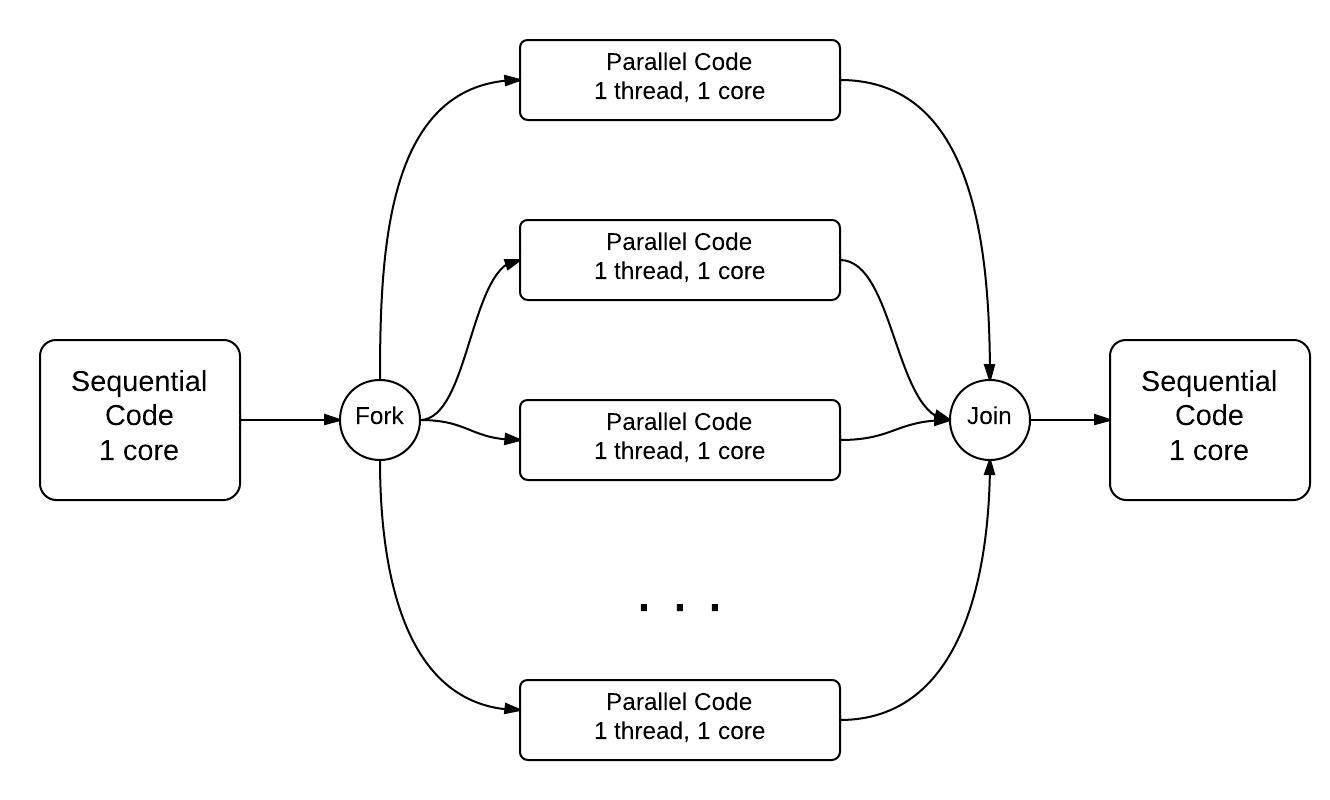
\includegraphics{ForkJoin.png}

Observe what happens on the machine
where you are running this code, both when you have the pragma commented (no fork) and when you uncomment it (adding a fork).

Note that in OpenMP the join is implicit and does not require a pragma directive.

\begin{Verbatim}[commandchars=\\\{\},numbers=left,firstnumber=1,stepnumber=1]
\PYG{c+cm}{/* forkJoin.c}
\PYG{c+cm}{ * ... illustrates the fork-join pattern }
\PYG{c+cm}{ *      using OpenMP's parallel directive.}
\PYG{c+cm}{ *}
\PYG{c+cm}{ * Joel Adams, Calvin College, November 2009.}
\PYG{c+cm}{ *}
\PYG{c+cm}{ * Usage: ./forkJoin}
\PYG{c+cm}{ *}
\PYG{c+cm}{ * Exercise:}
\PYG{c+cm}{ * - Compile \PYGZam{} run, uncomment the pragma,}
\PYG{c+cm}{ *    recompile \PYGZam{} run, compare results.}
\PYG{c+cm}{ */}

\PYG{c+cp}{\PYGZsh{}}\PYG{c+cp}{include \PYGZlt{}stdio.h\PYGZgt{}     }\PYG{c+c1}{// printf()}
\PYG{c+cp}{\PYGZsh{}}\PYG{c+cp}{include \PYGZlt{}omp.h\PYGZgt{}       }\PYG{c+c1}{// OpenMP}

\PYG{k+kt}{int} \PYG{n+nf}{main}\PYG{p}{(}\PYG{k+kt}{int} \PYG{n}{argc}\PYG{p}{,} \PYG{k+kt}{char}\PYG{o}{*}\PYG{o}{*} \PYG{n}{argv}\PYG{p}{)} \PYG{p}{\PYGZob{}}

    \PYG{n}{printf}\PYG{p}{(}\PYG{l+s}{"}\PYG{l+s+se}{\PYGZbs{}n}\PYG{l+s}{Before...}\PYG{l+s+se}{\PYGZbs{}n}\PYG{l+s}{"}\PYG{p}{)}\PYG{p}{;}

\PYG{c+c1}{//    \PYGZsh{}pragma omp parallel }
    \PYG{n}{printf}\PYG{p}{(}\PYG{l+s}{"}\PYG{l+s+se}{\PYGZbs{}n}\PYG{l+s}{During...}\PYG{l+s}{"}\PYG{p}{)}\PYG{p}{;}

    \PYG{n}{printf}\PYG{p}{(}\PYG{l+s}{"}\PYG{l+s+se}{\PYGZbs{}n}\PYG{l+s+se}{\PYGZbs{}n}\PYG{l+s}{After...}\PYG{l+s+se}{\PYGZbs{}n}\PYG{l+s+se}{\PYGZbs{}n}\PYG{l+s}{"}\PYG{p}{)}\PYG{p}{;}

    \PYG{k}{return} \PYG{l+m+mi}{0}\PYG{p}{;}
\PYG{p}{\PYGZcb{}}
\end{Verbatim}


\subsubsection{1. Program Structure Implementation Strategy: Fork-join with setting the number of threads}
\label{SharedMemory/ProgStructure_Barrier:program-structure-implementation-strategy-fork-join-with-setting-the-number-of-threads}
\emph{file openMP/01.forkJoin2/forkJoin2.c}

\emph{Build inside 01.forkJoin2 directory:}

\begin{Verbatim}[commandchars=\\\{\}]
make forkjoin2
\end{Verbatim}

\emph{Execute on the command line inside 01.forkJoin2 directory:}

\begin{Verbatim}[commandchars=\\\{\}]
./forkjoin2
\end{Verbatim}

This code illustrates that one program can fork and join more than once
and that programmers can set the number of threads to use in the parallel forked code.

Note on line 28 there is an OpenMP function called \emph{omp\_set\_num\_threads}
for setting the number of threads to use for each
\emph{fork}, which occur when the omp\_parallel pragma is used.
Also note on line 35 that you can set the number of threads for the very next
fork indicated by an omp\_parallel pragma by augmenting the pragma as shown in line 35.
Follow the instructions in the header of the code file to understand the difference
between these.

\begin{Verbatim}[commandchars=\\\{\},numbers=left,firstnumber=1,stepnumber=1]
\PYG{c+cm}{/* forkJoin2.c}
\PYG{c+cm}{ * ... illustrates the fork-join pattern }
\PYG{c+cm}{ *      using multiple OpenMP parallel directives,}
\PYG{c+cm}{ *      and changing the number of threads two ways.}
\PYG{c+cm}{ *}
\PYG{c+cm}{ * Joel Adams, Calvin College, May 2013.}
\PYG{c+cm}{ *}
\PYG{c+cm}{ * Usage: ./forkJoin2}
\PYG{c+cm}{ *}
\PYG{c+cm}{ * Exercise:}
\PYG{c+cm}{ * - Compile \PYGZam{} run, compare results to source.}
\PYG{c+cm}{ * - Predict how many threads will be used in 'Part IV'?}
\PYG{c+cm}{ * - Uncomment 'Part IV', recompile, rerun.}
\PYG{c+cm}{ */}

\PYG{c+cp}{\PYGZsh{}}\PYG{c+cp}{include \PYGZlt{}stdio.h\PYGZgt{}    }\PYG{c+c1}{// printf()}
\PYG{c+cp}{\PYGZsh{}}\PYG{c+cp}{include \PYGZlt{}omp.h\PYGZgt{}      }\PYG{c+c1}{// OpenMP}

\PYG{k+kt}{int} \PYG{n+nf}{main}\PYG{p}{(}\PYG{k+kt}{int} \PYG{n}{argc}\PYG{p}{,} \PYG{k+kt}{char}\PYG{o}{*}\PYG{o}{*} \PYG{n}{argv}\PYG{p}{)} \PYG{p}{\PYGZob{}}

    \PYG{n}{printf}\PYG{p}{(}\PYG{l+s}{"}\PYG{l+s+se}{\PYGZbs{}n}\PYG{l+s}{Beginning}\PYG{l+s+se}{\PYGZbs{}n}\PYG{l+s}{"}\PYG{p}{)}\PYG{p}{;}

    \PYG{c+cp}{\PYGZsh{}}\PYG{c+cp}{pragma omp parallel }
    \PYG{n}{printf}\PYG{p}{(}\PYG{l+s}{"}\PYG{l+s+se}{\PYGZbs{}n}\PYG{l+s}{Part I}\PYG{l+s}{"}\PYG{p}{)}\PYG{p}{;}

    \PYG{n}{printf}\PYG{p}{(}\PYG{l+s}{"}\PYG{l+s+se}{\PYGZbs{}n}\PYG{l+s+se}{\PYGZbs{}n}\PYG{l+s}{Between I and II...}\PYG{l+s+se}{\PYGZbs{}n}\PYG{l+s}{"}\PYG{p}{)}\PYG{p}{;}

    \PYG{n}{omp\PYGZus{}set\PYGZus{}num\PYGZus{}threads}\PYG{p}{(}\PYG{l+m+mi}{3}\PYG{p}{)}\PYG{p}{;}

    \PYG{c+cp}{\PYGZsh{}}\PYG{c+cp}{pragma omp parallel }
    \PYG{n}{printf}\PYG{p}{(}\PYG{l+s}{"}\PYG{l+s+se}{\PYGZbs{}n}\PYG{l+s}{Part II...}\PYG{l+s}{"}\PYG{p}{)}\PYG{p}{;}

    \PYG{n}{printf}\PYG{p}{(}\PYG{l+s}{"}\PYG{l+s+se}{\PYGZbs{}n}\PYG{l+s+se}{\PYGZbs{}n}\PYG{l+s}{Between II and III...}\PYG{l+s+se}{\PYGZbs{}n}\PYG{l+s}{"}\PYG{p}{)}\PYG{p}{;}

    \PYG{c+cp}{\PYGZsh{}}\PYG{c+cp}{pragma omp parallel num\PYGZus{}threads(5)}
    \PYG{n}{printf}\PYG{p}{(}\PYG{l+s}{"}\PYG{l+s+se}{\PYGZbs{}n}\PYG{l+s}{Part III...}\PYG{l+s}{"}\PYG{p}{)}\PYG{p}{;}
\PYG{c+cm}{/*}
\PYG{c+cm}{    printf("\PYGZbs{}n\PYGZbs{}nBetween III and IV...\PYGZbs{}n");}

\PYG{c+cm}{    \PYGZsh{}pragma omp parallel }
\PYG{c+cm}{    printf("\PYGZbs{}nPart IV...");}
\PYG{c+cm}{*/}
    \PYG{n}{printf}\PYG{p}{(}\PYG{l+s}{"}\PYG{l+s+se}{\PYGZbs{}n}\PYG{l+s+se}{\PYGZbs{}n}\PYG{l+s}{End}\PYG{l+s+se}{\PYGZbs{}n}\PYG{l+s+se}{\PYGZbs{}n}\PYG{l+s}{"}\PYG{p}{)}\PYG{p}{;}

    \PYG{k}{return} \PYG{l+m+mi}{0}\PYG{p}{;}
\PYG{p}{\PYGZcb{}}
\end{Verbatim}


\subsubsection{2. Program Structure Implementation Strategy: Single Program, multiple data}
\label{SharedMemory/ProgStructure_Barrier:program-structure-implementation-strategy-single-program-multiple-data}
\emph{file: openMP/02.spmd/spmd.c}

\emph{Build inside 02.spmd directory:}

\begin{Verbatim}[commandchars=\\\{\}]
make spmd
\end{Verbatim}

\emph{Execute on the command line inside 02.spmd directory:}

\begin{Verbatim}[commandchars=\\\{\}]
./spmd
\end{Verbatim}

Note how there are OpenMP functions to
obtain a thread number and the total number of threads.
We have one program, but multiple threads executing in the forked section,
each with a copy of the id and num\_threads variables.
Programmers write one program, but write it in such a way that
each thread has its own data values for particular variables.
This is why this is called the \emph{single program, multiple data} (SPMD) pattern.

Most parallel programs use this SPMD pattern, because writing one program
is ultimately the most efficient method for programmers.  It does require you
as a programmer to understand how this works, however.  Think carefully about
how each thread executing in parallel has its own set of variables.  Conceptually,
it looks like this, where each thread has its own memory for the variables id and numThreads:

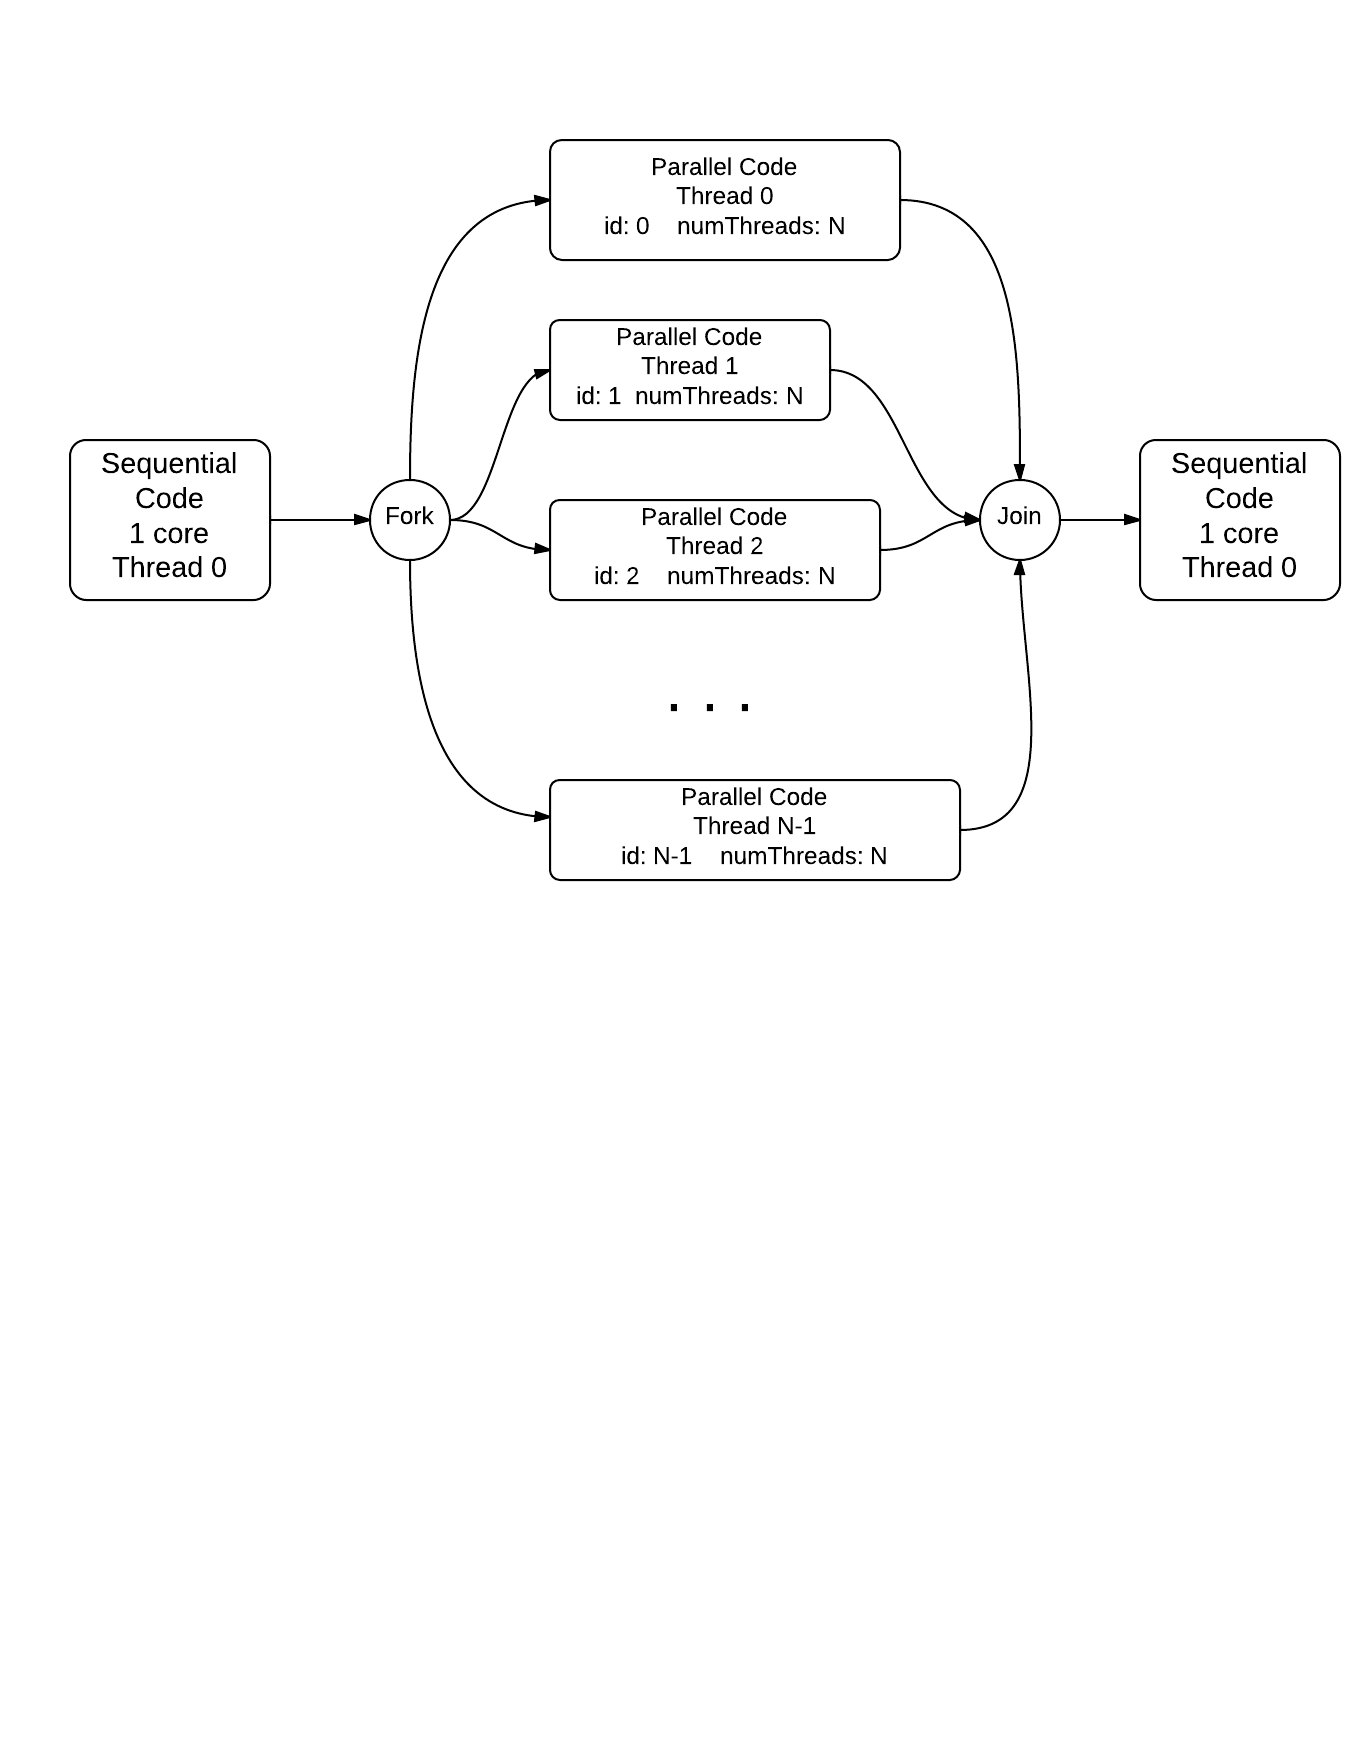
\includegraphics{ForkJoin_SPMD.png}

When the pragma is uncommented in the code below, note what the default number of threads
is.  Here the threads are forked and execute the block of code inside the
curly braces on lines 22 through 26.  This is how we can have a block of code executed
concurrently on each thread.

When you execute the parallel version containing the pragma (uncommenting line 20),
what do you observe about the order of the printed lines?  Run the program multiple times--
does the ordering change?  This illustrates an important point about threaded programs:
\emph{the ordering of execution of statements between threads is not guaranteed.}  This is also
illustrated in the diagram above.

\begin{Verbatim}[commandchars=\\\{\},numbers=left,firstnumber=1,stepnumber=1]
\PYG{c+cm}{/* spmd.c}
\PYG{c+cm}{ * ... illustrates the single-program-multiple-data (SPMD)}
\PYG{c+cm}{ *      pattern using two basic OpenMP commands...}
\PYG{c+cm}{ *}
\PYG{c+cm}{ * Joel Adams, Calvin College, November 2009.}
\PYG{c+cm}{ *}
\PYG{c+cm}{ * Usage: ./spmd}
\PYG{c+cm}{ *}
\PYG{c+cm}{ * Exercise:}
\PYG{c+cm}{ * - Compile \PYGZam{} run }
\PYG{c+cm}{ * - Uncomment pragma, recompile \PYGZam{} run, compare results}
\PYG{c+cm}{ */}

\PYG{c+cp}{\PYGZsh{}}\PYG{c+cp}{include \PYGZlt{}stdio.h\PYGZgt{}}
\PYG{c+cp}{\PYGZsh{}}\PYG{c+cp}{include \PYGZlt{}omp.h\PYGZgt{}}

\PYG{k+kt}{int} \PYG{n+nf}{main}\PYG{p}{(}\PYG{k+kt}{int} \PYG{n}{argc}\PYG{p}{,} \PYG{k+kt}{char}\PYG{o}{*}\PYG{o}{*} \PYG{n}{argv}\PYG{p}{)} \PYG{p}{\PYGZob{}}
    \PYG{n}{printf}\PYG{p}{(}\PYG{l+s}{"}\PYG{l+s+se}{\PYGZbs{}n}\PYG{l+s}{"}\PYG{p}{)}\PYG{p}{;}

\PYG{c+c1}{//    \PYGZsh{}pragma omp parallel }
    \PYG{p}{\PYGZob{}}
        \PYG{k+kt}{int} \PYG{n}{id} \PYG{o}{=} \PYG{n}{omp\PYGZus{}get\PYGZus{}thread\PYGZus{}num}\PYG{p}{(}\PYG{p}{)}\PYG{p}{;}
        \PYG{k+kt}{int} \PYG{n}{numThreads} \PYG{o}{=} \PYG{n}{omp\PYGZus{}get\PYGZus{}num\PYGZus{}threads}\PYG{p}{(}\PYG{p}{)}\PYG{p}{;}
        \PYG{n}{printf}\PYG{p}{(}\PYG{l+s}{"}\PYG{l+s}{Hello from thread \PYGZpc{}d of \PYGZpc{}d}\PYG{l+s+se}{\PYGZbs{}n}\PYG{l+s}{"}\PYG{p}{,} \PYG{n}{id}\PYG{p}{,} \PYG{n}{numThreads}\PYG{p}{)}\PYG{p}{;}
    \PYG{p}{\PYGZcb{}}

    \PYG{n}{printf}\PYG{p}{(}\PYG{l+s}{"}\PYG{l+s+se}{\PYGZbs{}n}\PYG{l+s}{"}\PYG{p}{)}\PYG{p}{;}
    \PYG{k}{return} \PYG{l+m+mi}{0}\PYG{p}{;}
\PYG{p}{\PYGZcb{}}
\end{Verbatim}


\subsubsection{3. Program Structure Implementation Strategy: Single Program, multiple data with user-defined number of threads}
\label{SharedMemory/ProgStructure_Barrier:program-structure-implementation-strategy-single-program-multiple-data-with-user-defined-number-of-threads}
\emph{file: openMP/03.spmd2/spmd2.c}

\emph{Build inside 03.spmd2 directory:}

\begin{Verbatim}[commandchars=\\\{\}]
make spmd2
\end{Verbatim}

\emph{Execute on the command line inside 03.spmd2 directory:}

\begin{Verbatim}[commandchars=\\\{\}]
./spmd2 4
Replace 4 with other values for the number of threads
\end{Verbatim}

Here we enter the number of threads to use on the command line.  This is a useful way to
make your code versatile so that you can use as many threads as you would like.

\begin{Verbatim}[commandchars=\\\{\},numbers=left,firstnumber=1,stepnumber=1]
\PYG{c+cm}{/* spmd2.c}
\PYG{c+cm}{ * ... illustrates the SPMD pattern in OpenMP,}
\PYG{c+cm}{ * 	using the commandline arguments }
\PYG{c+cm}{ *      to control the number of threads.}
\PYG{c+cm}{ *}
\PYG{c+cm}{ * Joel Adams, Calvin College, November 2009.}
\PYG{c+cm}{ *}
\PYG{c+cm}{ * Usage: ./spmd2 [numThreads]}
\PYG{c+cm}{ *}
\PYG{c+cm}{ * Exercise:}
\PYG{c+cm}{ * - Compile \PYGZam{} run with no commandline args }
\PYG{c+cm}{ * - Rerun with different commandline args}
\PYG{c+cm}{ */}

\PYG{c+cp}{\PYGZsh{}}\PYG{c+cp}{include \PYGZlt{}stdio.h\PYGZgt{}}
\PYG{c+cp}{\PYGZsh{}}\PYG{c+cp}{include \PYGZlt{}omp.h\PYGZgt{}}
\PYG{c+cp}{\PYGZsh{}}\PYG{c+cp}{include \PYGZlt{}stdlib.h\PYGZgt{}}

\PYG{k+kt}{int} \PYG{n+nf}{main}\PYG{p}{(}\PYG{k+kt}{int} \PYG{n}{argc}\PYG{p}{,} \PYG{k+kt}{char}\PYG{o}{*}\PYG{o}{*} \PYG{n}{argv}\PYG{p}{)} \PYG{p}{\PYGZob{}}
    \PYG{k+kt}{int} \PYG{n}{id}\PYG{p}{,} \PYG{n}{numThreads}\PYG{p}{;}

    \PYG{n}{printf}\PYG{p}{(}\PYG{l+s}{"}\PYG{l+s+se}{\PYGZbs{}n}\PYG{l+s}{"}\PYG{p}{)}\PYG{p}{;}
    \PYG{k}{if} \PYG{p}{(}\PYG{n}{argc} \PYG{o}{\PYGZgt{}} \PYG{l+m+mi}{1}\PYG{p}{)} \PYG{p}{\PYGZob{}}
        \PYG{n}{omp\PYGZus{}set\PYGZus{}num\PYGZus{}threads}\PYG{p}{(} \PYG{n}{atoi}\PYG{p}{(}\PYG{n}{argv}\PYG{p}{[}\PYG{l+m+mi}{1}\PYG{p}{]}\PYG{p}{)} \PYG{p}{)}\PYG{p}{;}
    \PYG{p}{\PYGZcb{}}

    \PYG{c+cp}{\PYGZsh{}}\PYG{c+cp}{pragma omp parallel }
    \PYG{p}{\PYGZob{}}
        \PYG{n}{id} \PYG{o}{=} \PYG{n}{omp\PYGZus{}get\PYGZus{}thread\PYGZus{}num}\PYG{p}{(}\PYG{p}{)}\PYG{p}{;}
        \PYG{n}{numThreads} \PYG{o}{=} \PYG{n}{omp\PYGZus{}get\PYGZus{}num\PYGZus{}threads}\PYG{p}{(}\PYG{p}{)}\PYG{p}{;}
        \PYG{n}{printf}\PYG{p}{(}\PYG{l+s}{"}\PYG{l+s}{Hello from thread \PYGZpc{}d of \PYGZpc{}d}\PYG{l+s+se}{\PYGZbs{}n}\PYG{l+s}{"}\PYG{p}{,} \PYG{n}{id}\PYG{p}{,} \PYG{n}{numThreads}\PYG{p}{)}\PYG{p}{;}
    \PYG{p}{\PYGZcb{}}

    \PYG{n}{printf}\PYG{p}{(}\PYG{l+s}{"}\PYG{l+s+se}{\PYGZbs{}n}\PYG{l+s}{"}\PYG{p}{)}\PYG{p}{;}
    \PYG{k}{return} \PYG{l+m+mi}{0}\PYG{p}{;}
\PYG{p}{\PYGZcb{}}
\end{Verbatim}


\subsubsection{4. Coordination: Synchronization with a Barrier}
\label{SharedMemory/ProgStructure_Barrier:coordination-synchronization-with-a-barrier}
\emph{file: openMP/04.barrier/barrier.c}

\emph{Build inside 04.barrier directory:}

\begin{Verbatim}[commandchars=\\\{\}]
make barrier
\end{Verbatim}

\emph{Execute on the command line inside 04.barrier directory:}

\begin{Verbatim}[commandchars=\\\{\}]
./barrier 4
Replace 4 with other values for the number of threads
\end{Verbatim}

The barrier pattern is used in parallel programs to ensure that all threads complete
a parallel section of code before execution continues. This can be necessary when
threads are generating computed data (in an array, for example) that needs to be
completed for use in another computation.

Conceptually, the running code is excuting like this:

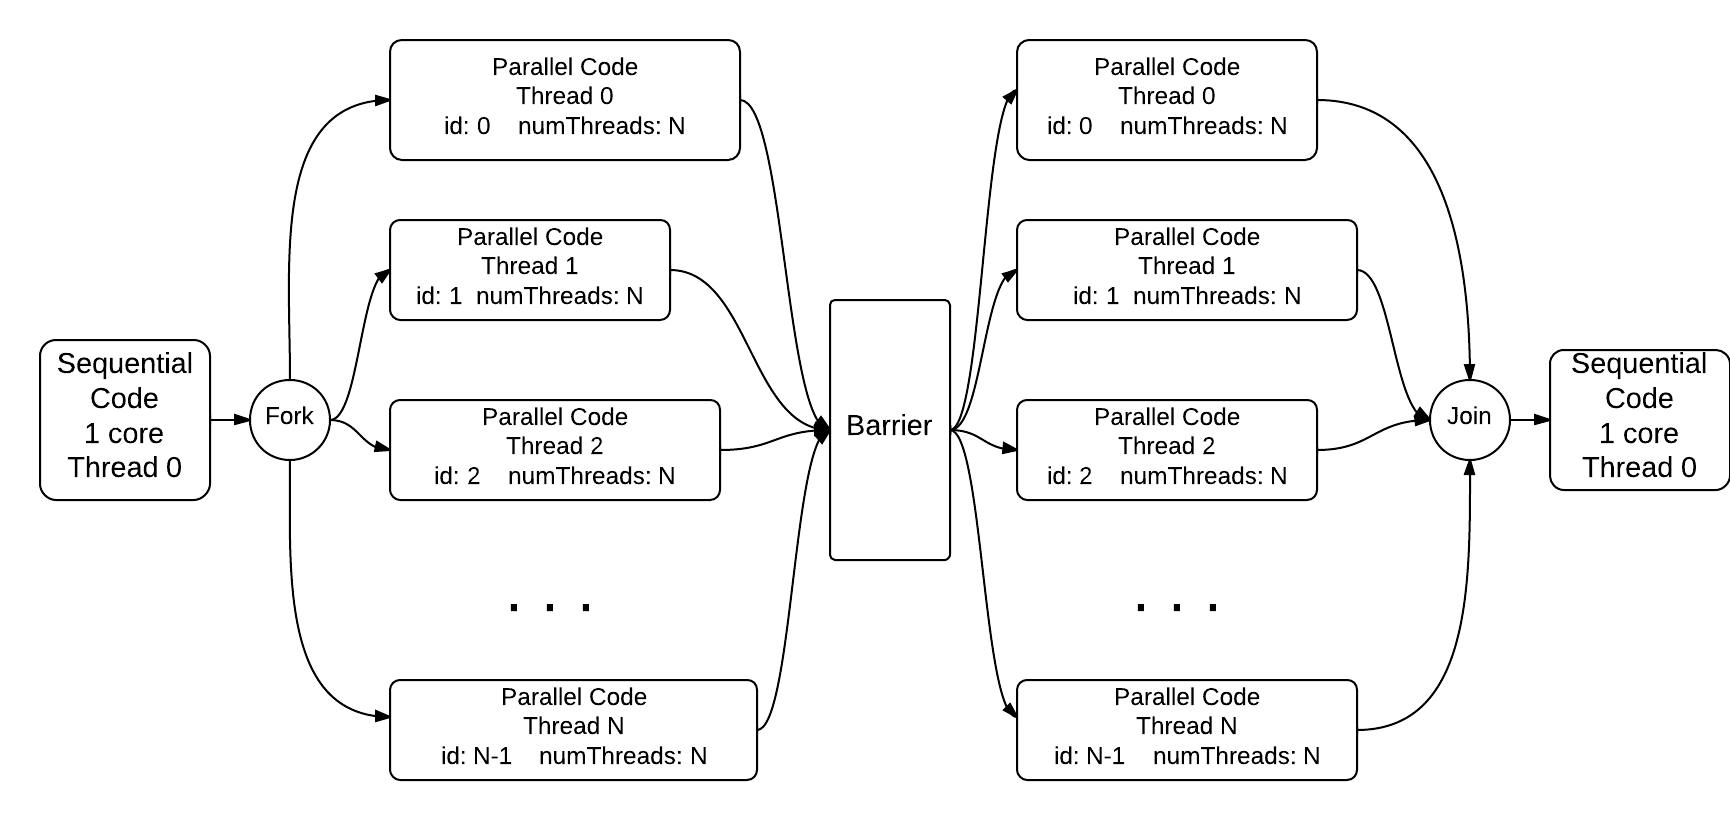
\includegraphics{ForkJoin_Barrier.png}

Note what happens with and without the commented pragma on line 31.

\begin{Verbatim}[commandchars=\\\{\},numbers=left,firstnumber=1,stepnumber=1]
\PYG{c+cm}{/* barrier.c}
\PYG{c+cm}{ * ... illustrates the use of the OpenMP barrier command,}
\PYG{c+cm}{ * 	using the commandline to control the number of threads...}
\PYG{c+cm}{ *}
\PYG{c+cm}{ * Joel Adams, Calvin College, May 2013.}
\PYG{c+cm}{ *}
\PYG{c+cm}{ * Usage: ./barrier [numThreads]}
\PYG{c+cm}{ * }
\PYG{c+cm}{ * Exercise:}
\PYG{c+cm}{ * - Compile \PYGZam{} run several times, noting interleaving of outputs.}
\PYG{c+cm}{ * - Uncomment the barrier directive, recompile, rerun,}
\PYG{c+cm}{ *    and note the change in the outputs.}
\PYG{c+cm}{ */}

\PYG{c+cp}{\PYGZsh{}}\PYG{c+cp}{include \PYGZlt{}stdio.h\PYGZgt{}}
\PYG{c+cp}{\PYGZsh{}}\PYG{c+cp}{include \PYGZlt{}omp.h\PYGZgt{}}
\PYG{c+cp}{\PYGZsh{}}\PYG{c+cp}{include \PYGZlt{}stdlib.h\PYGZgt{}}

\PYG{k+kt}{int} \PYG{n+nf}{main}\PYG{p}{(}\PYG{k+kt}{int} \PYG{n}{argc}\PYG{p}{,} \PYG{k+kt}{char}\PYG{o}{*}\PYG{o}{*} \PYG{n}{argv}\PYG{p}{)} \PYG{p}{\PYGZob{}}
    \PYG{n}{printf}\PYG{p}{(}\PYG{l+s}{"}\PYG{l+s+se}{\PYGZbs{}n}\PYG{l+s}{"}\PYG{p}{)}\PYG{p}{;}
    \PYG{k}{if} \PYG{p}{(}\PYG{n}{argc} \PYG{o}{\PYGZgt{}} \PYG{l+m+mi}{1}\PYG{p}{)} \PYG{p}{\PYGZob{}}
        \PYG{n}{omp\PYGZus{}set\PYGZus{}num\PYGZus{}threads}\PYG{p}{(} \PYG{n}{atoi}\PYG{p}{(}\PYG{n}{argv}\PYG{p}{[}\PYG{l+m+mi}{1}\PYG{p}{]}\PYG{p}{)} \PYG{p}{)}\PYG{p}{;}
    \PYG{p}{\PYGZcb{}}

    \PYG{c+cp}{\PYGZsh{}}\PYG{c+cp}{pragma omp parallel }
    \PYG{p}{\PYGZob{}}
        \PYG{k+kt}{int} \PYG{n}{id} \PYG{o}{=} \PYG{n}{omp\PYGZus{}get\PYGZus{}thread\PYGZus{}num}\PYG{p}{(}\PYG{p}{)}\PYG{p}{;}
        \PYG{k+kt}{int} \PYG{n}{numThreads} \PYG{o}{=} \PYG{n}{omp\PYGZus{}get\PYGZus{}num\PYGZus{}threads}\PYG{p}{(}\PYG{p}{)}\PYG{p}{;}
        \PYG{n}{printf}\PYG{p}{(}\PYG{l+s}{"}\PYG{l+s}{Thread \PYGZpc{}d of \PYGZpc{}d is BEFORE the barrier.}\PYG{l+s+se}{\PYGZbs{}n}\PYG{l+s}{"}\PYG{p}{,} \PYG{n}{id}\PYG{p}{,} \PYG{n}{numThreads}\PYG{p}{)}\PYG{p}{;}

\PYG{c+c1}{//        \PYGZsh{}pragma omp barrier }

        \PYG{n}{printf}\PYG{p}{(}\PYG{l+s}{"}\PYG{l+s}{Thread \PYGZpc{}d of \PYGZpc{}d is AFTER the barrier.}\PYG{l+s+se}{\PYGZbs{}n}\PYG{l+s}{"}\PYG{p}{,} \PYG{n}{id}\PYG{p}{,} \PYG{n}{numThreads}\PYG{p}{)}\PYG{p}{;}
    \PYG{p}{\PYGZcb{}}

    \PYG{n}{printf}\PYG{p}{(}\PYG{l+s}{"}\PYG{l+s+se}{\PYGZbs{}n}\PYG{l+s}{"}\PYG{p}{)}\PYG{p}{;}
    \PYG{k}{return} \PYG{l+m+mi}{0}\PYG{p}{;}
\PYG{p}{\PYGZcb{}}
\end{Verbatim}


\subsubsection{5. Program Structure: The Master-Worker Implementation Strategy}
\label{SharedMemory/ProgStructure_Barrier:program-structure-the-master-worker-implementation-strategy}
\emph{file: openMP/05.masterWorker/masterWorker.c}

\emph{Build inside 05.masterWorker directory:}

\begin{Verbatim}[commandchars=\\\{\}]
make masterWorker
\end{Verbatim}

\emph{Execute on the command line inside 05.masterWorker directory:}

\begin{Verbatim}[commandchars=\\\{\}]
./masterWorker 4
Replace 4 with other values for the number of threads
\end{Verbatim}

Once you have mastered the notion of fork-join and single-program, multiple data,
the next common pattern that programmers use in association with these patterns
is to have one thread, called the master, execute one block of code when it forks while the rest
of the threads, called workers, execute a different block of code when they fork.
This is illustrated in this simple example (useful code would be more complicated).

\begin{Verbatim}[commandchars=\\\{\},numbers=left,firstnumber=1,stepnumber=1]
\PYG{c+cm}{/* masterWorker.c}
\PYG{c+cm}{ * ... illustrates the master-worker pattern in OpenMP}
\PYG{c+cm}{ *}
\PYG{c+cm}{ * Joel Adams, Calvin College, November 2009.}
\PYG{c+cm}{ *}
\PYG{c+cm}{ * Usage: ./masterWorker}
\PYG{c+cm}{ *}
\PYG{c+cm}{ * Exercise: }
\PYG{c+cm}{ * - Compile and run as is.}
\PYG{c+cm}{ * - Uncomment \PYGZsh{}pragma directive, re-compile and re-run}
\PYG{c+cm}{ * - Compare and trace the different executions.}
\PYG{c+cm}{ */}

\PYG{c+cp}{\PYGZsh{}}\PYG{c+cp}{include \PYGZlt{}stdio.h\PYGZgt{}   }\PYG{c+c1}{// printf()}
\PYG{c+cp}{\PYGZsh{}}\PYG{c+cp}{include \PYGZlt{}stdlib.h\PYGZgt{}   }\PYG{c+c1}{// atoi()}
\PYG{c+cp}{\PYGZsh{}}\PYG{c+cp}{include \PYGZlt{}omp.h\PYGZgt{}     }\PYG{c+c1}{// OpenMP}

\PYG{k+kt}{int} \PYG{n+nf}{main}\PYG{p}{(}\PYG{k+kt}{int} \PYG{n}{argc}\PYG{p}{,} \PYG{k+kt}{char}\PYG{o}{*}\PYG{o}{*} \PYG{n}{argv}\PYG{p}{)} \PYG{p}{\PYGZob{}}
    \PYG{n}{printf}\PYG{p}{(}\PYG{l+s}{"}\PYG{l+s+se}{\PYGZbs{}n}\PYG{l+s}{"}\PYG{p}{)}\PYG{p}{;}
    \PYG{k}{if} \PYG{p}{(}\PYG{n}{argc} \PYG{o}{\PYGZgt{}} \PYG{l+m+mi}{1}\PYG{p}{)} \PYG{p}{\PYGZob{}}
        \PYG{n}{omp\PYGZus{}set\PYGZus{}num\PYGZus{}threads}\PYG{p}{(} \PYG{n}{atoi}\PYG{p}{(}\PYG{n}{argv}\PYG{p}{[}\PYG{l+m+mi}{1}\PYG{p}{]}\PYG{p}{)} \PYG{p}{)}\PYG{p}{;}
    \PYG{p}{\PYGZcb{}}

\PYG{c+c1}{//    \PYGZsh{}pragma omp parallel }
    \PYG{p}{\PYGZob{}}
        \PYG{k+kt}{int} \PYG{n}{id} \PYG{o}{=} \PYG{n}{omp\PYGZus{}get\PYGZus{}thread\PYGZus{}num}\PYG{p}{(}\PYG{p}{)}\PYG{p}{;}
        \PYG{k+kt}{int} \PYG{n}{numThreads} \PYG{o}{=} \PYG{n}{omp\PYGZus{}get\PYGZus{}num\PYGZus{}threads}\PYG{p}{(}\PYG{p}{)}\PYG{p}{;}

        \PYG{k}{if} \PYG{p}{(} \PYG{n}{id} \PYG{o}{=}\PYG{o}{=} \PYG{l+m+mi}{0} \PYG{p}{)} \PYG{p}{\PYGZob{}}  \PYG{c+c1}{// thread with ID 0 is master}
            \PYG{n}{printf}\PYG{p}{(}\PYG{l+s}{"}\PYG{l+s}{Greetings from the master, \PYGZsh{} \PYGZpc{}d of \PYGZpc{}d threads}\PYG{l+s+se}{\PYGZbs{}n}\PYG{l+s}{"}\PYG{p}{,}
			    \PYG{n}{id}\PYG{p}{,} \PYG{n}{numThreads}\PYG{p}{)}\PYG{p}{;}
        \PYG{p}{\PYGZcb{}} \PYG{k}{else} \PYG{p}{\PYGZob{}}          \PYG{c+c1}{// threads with IDs \PYGZgt{} 0 are workers }
            \PYG{n}{printf}\PYG{p}{(}\PYG{l+s}{"}\PYG{l+s}{Greetings from a worker, \PYGZsh{} \PYGZpc{}d of \PYGZpc{}d threads}\PYG{l+s+se}{\PYGZbs{}n}\PYG{l+s}{"}\PYG{p}{,}
			    \PYG{n}{id}\PYG{p}{,} \PYG{n}{numThreads}\PYG{p}{)}\PYG{p}{;}
        \PYG{p}{\PYGZcb{}}
    \PYG{p}{\PYGZcb{}}

    \PYG{n}{printf}\PYG{p}{(}\PYG{l+s}{"}\PYG{l+s+se}{\PYGZbs{}n}\PYG{l+s}{"}\PYG{p}{)}\PYG{p}{;}

    \PYG{k}{return} \PYG{l+m+mi}{0}\PYG{p}{;}
\PYG{p}{\PYGZcb{}}
\end{Verbatim}


\subsection{Data Decomposition Algorithm Strategies and Related Coordination Strategies}
\label{SharedMemory/DataDecomp_Reduction::doc}\label{SharedMemory/DataDecomp_Reduction:data-decomposition-algorithm-strategies-and-related-coordination-strategies}

\subsubsection{6. Shared Data Decomposition Algorithm Strategy:  chunks of data per thread using a parallel for loop implementation strategy}
\label{SharedMemory/DataDecomp_Reduction:shared-data-decomposition-algorithm-strategy-chunks-of-data-per-thread-using-a-parallel-for-loop-implementation-strategy}
\emph{file: openMP/06.parallelLoop-equalChunks/parallelLoopEqualChunks.c}

\emph{Build inside 06.parallelLoop-equalChunks directory:}

\begin{Verbatim}[commandchars=\\\{\}]
make parallelLoopEqualChunks
\end{Verbatim}

\emph{Execute on the command line inside 06.parallelLoop-equalChunks directory:}

\begin{Verbatim}[commandchars=\\\{\}]
./parallelLoopEqualChunks 4
Replace 4 with other values for the number of threads, or leave off
\end{Verbatim}

An iterative for loop is a remarkably common pattern in all programming, primarily used to
perform a calculation N times, often over a set of data containing N elements, using each
element in turn inside the for loop.  If there are no dependencies between the calculations
(i.e. the order of them is not important), then the code inside the loop can be split
between forked threads.  When doing this, a decision the programmer needs to make is to
decide how to partition the work between the threads by answering this question:
\begin{itemize}
\item {} 
How many and which iterations of the loop will each thread complete on its own?

\end{itemize}

We refer to this as the \textbf{data decomposition} pattern because we are decomposing the
amount of work to be done (typically on a set of data) across multiple threads.
In the following code, this is done in OpenMP using the \emph{omp parallel for} pragma
just in front of the for statement (line 27) in the following code.

\begin{Verbatim}[commandchars=\\\{\},numbers=left,firstnumber=1,stepnumber=1]
\PYG{c+cm}{/* parallelLoopEqualChunks.c}
\PYG{c+cm}{ * ... illustrates the use of OpenMP's default parallel for loop in which}
\PYG{c+cm}{ *  	threads iterate through equal sized chunks of the index range}
\PYG{c+cm}{ *	(cache-beneficial when accessing adjacent memory locations).}
\PYG{c+cm}{ *}
\PYG{c+cm}{ * Joel Adams, Calvin College, November 2009.}
\PYG{c+cm}{ *}
\PYG{c+cm}{ * Usage: ./parallelLoopEqualChunks [numThreads]}
\PYG{c+cm}{ *}
\PYG{c+cm}{ * Exercise}
\PYG{c+cm}{ * - Compile and run, comparing output to source code}
\PYG{c+cm}{ * - try with different numbers of threads, e.g.: 2, 3, 4, 6, 8}
\PYG{c+cm}{ */}

\PYG{c+cp}{\PYGZsh{}}\PYG{c+cp}{include \PYGZlt{}stdio.h\PYGZgt{}    }\PYG{c+c1}{// printf()}
\PYG{c+cp}{\PYGZsh{}}\PYG{c+cp}{include \PYGZlt{}stdlib.h\PYGZgt{}   }\PYG{c+c1}{// atoi()}
\PYG{c+cp}{\PYGZsh{}}\PYG{c+cp}{include \PYGZlt{}omp.h\PYGZgt{}      }\PYG{c+c1}{// OpenMP}

\PYG{k+kt}{int} \PYG{n+nf}{main}\PYG{p}{(}\PYG{k+kt}{int} \PYG{n}{argc}\PYG{p}{,} \PYG{k+kt}{char}\PYG{o}{*}\PYG{o}{*} \PYG{n}{argv}\PYG{p}{)} \PYG{p}{\PYGZob{}}
    \PYG{k}{const} \PYG{k+kt}{int} \PYG{n}{REPS} \PYG{o}{=} \PYG{l+m+mi}{16}\PYG{p}{;}

    \PYG{n}{printf}\PYG{p}{(}\PYG{l+s}{"}\PYG{l+s+se}{\PYGZbs{}n}\PYG{l+s}{"}\PYG{p}{)}\PYG{p}{;}
    \PYG{k}{if} \PYG{p}{(}\PYG{n}{argc} \PYG{o}{\PYGZgt{}} \PYG{l+m+mi}{1}\PYG{p}{)} \PYG{p}{\PYGZob{}}
        \PYG{n}{omp\PYGZus{}set\PYGZus{}num\PYGZus{}threads}\PYG{p}{(} \PYG{n}{atoi}\PYG{p}{(}\PYG{n}{argv}\PYG{p}{[}\PYG{l+m+mi}{1}\PYG{p}{]}\PYG{p}{)} \PYG{p}{)}\PYG{p}{;}
    \PYG{p}{\PYGZcb{}}

    \PYG{c+cp}{\PYGZsh{}}\PYG{c+cp}{pragma omp parallel for  }
    \PYG{k}{for} \PYG{p}{(}\PYG{k+kt}{int} \PYG{n}{i} \PYG{o}{=} \PYG{l+m+mi}{0}\PYG{p}{;} \PYG{n}{i} \PYG{o}{\PYGZlt{}} \PYG{n}{REPS}\PYG{p}{;} \PYG{n}{i}\PYG{o}{+}\PYG{o}{+}\PYG{p}{)} \PYG{p}{\PYGZob{}}
        \PYG{k+kt}{int} \PYG{n}{id} \PYG{o}{=} \PYG{n}{omp\PYGZus{}get\PYGZus{}thread\PYGZus{}num}\PYG{p}{(}\PYG{p}{)}\PYG{p}{;}
        \PYG{n}{printf}\PYG{p}{(}\PYG{l+s}{"}\PYG{l+s}{Thread \PYGZpc{}d performed iteration \PYGZpc{}d}\PYG{l+s+se}{\PYGZbs{}n}\PYG{l+s}{"}\PYG{p}{,} 
                 \PYG{n}{id}\PYG{p}{,} \PYG{n}{i}\PYG{p}{)}\PYG{p}{;}
    \PYG{p}{\PYGZcb{}}

    \PYG{n}{printf}\PYG{p}{(}\PYG{l+s}{"}\PYG{l+s+se}{\PYGZbs{}n}\PYG{l+s}{"}\PYG{p}{)}\PYG{p}{;}
    \PYG{k}{return} \PYG{l+m+mi}{0}\PYG{p}{;}
\PYG{p}{\PYGZcb{}}
\end{Verbatim}

Once you run this code, verify that the default behavior for this pragma is this
sort of decomposition of iterations of the loop to threads, when you set the
number of threads to 4 on the command line:

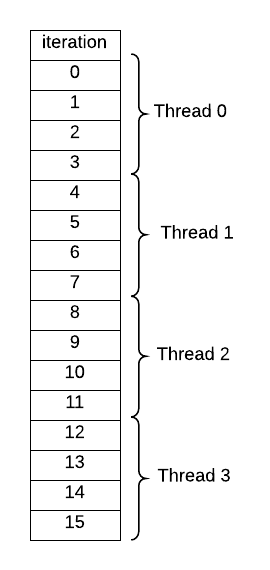
\includegraphics{ParalleFor_Chunks-4_threads-1.png}

What happens when the number of iterations (16 in this code) is not evenly divisible by the number of threads?  Try several cases to be certain how the compiler splits up the work.
This type of decomposition is commonly used when accessing data that is stored in
consecutive memory locations (such as an array) that might be cached by each thread.


\subsubsection{7. Shared Data Decomposition Algorithm Strategy:  one iteration per thread in a parallel for loop implementation strategy}
\label{SharedMemory/DataDecomp_Reduction:shared-data-decomposition-algorithm-strategy-one-iteration-per-thread-in-a-parallel-for-loop-implementation-strategy}
\emph{file: openMP/07.parallelLoop-chunksOf1/parallelLoopChunksOf1.c}

\emph{Build inside 07.parallelLoop-chunksOf1 directory:}

\begin{Verbatim}[commandchars=\\\{\}]
make parallelLoopChunksOf1
\end{Verbatim}

\emph{Execute on the command line inside 07.parallelLoop-chunksOf1 directory:}

\begin{Verbatim}[commandchars=\\\{\}]
./parallelLoopChunksOf1 4
Replace 4 with other values for the number of threads, or leave off
\end{Verbatim}

You can imagine other ways of assigning threads to iterations of a loop besides that
shown above for four threads and 16 iterations.  A simple decomposition sometimes used
when your loop is not accessing consecutive memory locations would be to let each
thread do one iteration, up to N threads, then
start again with thread 0 taking the next iteration.  This is declared in OpenMP
using the pragma on line 31 of the following code.  Also note that the commented code
below it is an alternative explicit way of doing it.  The schedule clause is the preferred style
when using OpenMP and is more versatile, because you can easily change the \emph{chunk size}
that each thread will work on.

\begin{Verbatim}[commandchars=\\\{\},numbers=left,firstnumber=1,stepnumber=1]
\PYG{c+cm}{/* parallelLoopChunksOf1.c}
\PYG{c+cm}{ * ... illustrates how to make OpenMP map threads to }
\PYG{c+cm}{ *	parallel loop iterations in chunks of size 1}
\PYG{c+cm}{ *	(use when not accesssing memory).}
\PYG{c+cm}{ *}
\PYG{c+cm}{ * Joel Adams, Calvin College, November 2009.}
\PYG{c+cm}{ *}
\PYG{c+cm}{ * Usage: ./parallelLoopChunksOf1 [numThreads]}
\PYG{c+cm}{ *}
\PYG{c+cm}{ * Exercise:}
\PYG{c+cm}{ * 1. Compile and run, comparing output to source code,}
\PYG{c+cm}{ *    and to the output of the 'equal chunks' version.}
\PYG{c+cm}{ * 2. Uncomment the "commented out" code below,}
\PYG{c+cm}{ *    and verify that both loops produce the same output.}
\PYG{c+cm}{ *    The first loop is simpler but more restrictive;}
\PYG{c+cm}{ *    the second loop is more complex but less restrictive.}
\PYG{c+cm}{ */}

\PYG{c+cp}{\PYGZsh{}}\PYG{c+cp}{include \PYGZlt{}stdio.h\PYGZgt{}}
\PYG{c+cp}{\PYGZsh{}}\PYG{c+cp}{include \PYGZlt{}omp.h\PYGZgt{}}
\PYG{c+cp}{\PYGZsh{}}\PYG{c+cp}{include \PYGZlt{}stdlib.h\PYGZgt{}}

\PYG{k+kt}{int} \PYG{n+nf}{main}\PYG{p}{(}\PYG{k+kt}{int} \PYG{n}{argc}\PYG{p}{,} \PYG{k+kt}{char}\PYG{o}{*}\PYG{o}{*} \PYG{n}{argv}\PYG{p}{)} \PYG{p}{\PYGZob{}}
    \PYG{k}{const} \PYG{k+kt}{int} \PYG{n}{REPS} \PYG{o}{=} \PYG{l+m+mi}{16}\PYG{p}{;}

    \PYG{n}{printf}\PYG{p}{(}\PYG{l+s}{"}\PYG{l+s+se}{\PYGZbs{}n}\PYG{l+s}{"}\PYG{p}{)}\PYG{p}{;}
    \PYG{k}{if} \PYG{p}{(}\PYG{n}{argc} \PYG{o}{\PYGZgt{}} \PYG{l+m+mi}{1}\PYG{p}{)} \PYG{p}{\PYGZob{}}
        \PYG{n}{omp\PYGZus{}set\PYGZus{}num\PYGZus{}threads}\PYG{p}{(} \PYG{n}{atoi}\PYG{p}{(}\PYG{n}{argv}\PYG{p}{[}\PYG{l+m+mi}{1}\PYG{p}{]}\PYG{p}{)} \PYG{p}{)}\PYG{p}{;}
    \PYG{p}{\PYGZcb{}}

    \PYG{c+cp}{\PYGZsh{}}\PYG{c+cp}{pragma omp parallel for schedule(static,1)}
    \PYG{k}{for} \PYG{p}{(}\PYG{k+kt}{int} \PYG{n}{i} \PYG{o}{=} \PYG{l+m+mi}{0}\PYG{p}{;} \PYG{n}{i} \PYG{o}{\PYGZlt{}} \PYG{n}{REPS}\PYG{p}{;} \PYG{n}{i}\PYG{o}{+}\PYG{o}{+}\PYG{p}{)} \PYG{p}{\PYGZob{}}
        \PYG{k+kt}{int} \PYG{n}{id} \PYG{o}{=} \PYG{n}{omp\PYGZus{}get\PYGZus{}thread\PYGZus{}num}\PYG{p}{(}\PYG{p}{)}\PYG{p}{;}
        \PYG{n}{printf}\PYG{p}{(}\PYG{l+s}{"}\PYG{l+s}{Thread \PYGZpc{}d performed iteration \PYGZpc{}d}\PYG{l+s+se}{\PYGZbs{}n}\PYG{l+s}{"}\PYG{p}{,} 
                 \PYG{n}{id}\PYG{p}{,} \PYG{n}{i}\PYG{p}{)}\PYG{p}{;}
    \PYG{p}{\PYGZcb{}}

\PYG{c+cm}{/*}
\PYG{c+cm}{    printf("\PYGZbs{}n---\PYGZbs{}n\PYGZbs{}n");}

\PYG{c+cm}{    \PYGZsh{}pragma omp parallel}
\PYG{c+cm}{    \PYGZob{}}
\PYG{c+cm}{        int id = omp\PYGZus{}get\PYGZus{}thread\PYGZus{}num();}
\PYG{c+cm}{        int numThreads = omp\PYGZus{}get\PYGZus{}num\PYGZus{}threads();}
\PYG{c+cm}{        for (int i = id; i \PYGZlt{} REPS; i += numThreads) \PYGZob{}}
\PYG{c+cm}{            printf("Thread \PYGZpc{}d performed iteration \PYGZpc{}d\PYGZbs{}n", }
\PYG{c+cm}{                     id, i);}
\PYG{c+cm}{        \PYGZcb{}}
\PYG{c+cm}{    \PYGZcb{}}
\PYG{c+cm}{*/}
    \PYG{n}{printf}\PYG{p}{(}\PYG{l+s}{"}\PYG{l+s+se}{\PYGZbs{}n}\PYG{l+s}{"}\PYG{p}{)}\PYG{p}{;}
    \PYG{k}{return} \PYG{l+m+mi}{0}\PYG{p}{;}
\PYG{p}{\PYGZcb{}}
\end{Verbatim}

This can be made even more
efficient if the next available thread simply takes the next iteration.
In OpenMP, this is done by using \emph{dynamic} scheduling instead of the static scheduling shown
in the above code.  Also note that the number of iterations, or chunk size, could
be greater than 1 inside the schedule clause.


\subsubsection{8. Coordination Using Collective Communication: Reduction}
\label{SharedMemory/DataDecomp_Reduction:coordination-using-collective-communication-reduction}
\emph{file: openMP/08.reduction/reduction.c}

\emph{Build inside 08.reduction directory:}

\begin{Verbatim}[commandchars=\\\{\}]
make reduction
\end{Verbatim}

\emph{Execute on the command line inside 08.reduction directory:}

\begin{Verbatim}[commandchars=\\\{\}]
./reduction 4
Replace 4 with other values for the number of threads, or leave off
\end{Verbatim}

Once threads have performed independent concurrent computations, possibly
on some portion of decomposed data, it is quite common to then \emph{reduce}
those individual computations into one value. This type of operation is
called a \textbf{collective communication} pattern because the threads must somehow
work together to create the final desired single value.

In this example, an array of randomly assigned integers represents a set of shared data (a more realistic program would perform a computation
that creates meaningful data values; this is just an example).
Note the common sequential code pattern found in the function called \emph{sequentialSum} in the code
below (starting line 51): a for loop is used to sum up all the values in the array.

Next let's consider how this can be done in parallel with threads.
Somehow the threads must implicitly \emph{communicate} to keep the overall sum updated
as each of them works on a portion of the array.
In the \emph{parallelSum} function, line 64 shows a special clause that
can be used with the parallel for pragma in OpenMP for this. All values
in the array are summed together by using the OpenMP
parallel for pragma with the \emph{reduction(+:sum)} clause on the variable \textbf{sum},
which is computed in line 66.

\begin{Verbatim}[commandchars=\\\{\},numbers=left,firstnumber=1,stepnumber=1]
\PYG{c+cm}{/* reduction.c}
\PYG{c+cm}{ * ... illustrates the OpenMP parallel-for loop's reduction clause}
\PYG{c+cm}{ *}
\PYG{c+cm}{ * Joel Adams, Calvin College, November 2009.}
\PYG{c+cm}{ *}
\PYG{c+cm}{ * Usage: ./reduction }
\PYG{c+cm}{ *}
\PYG{c+cm}{ * Exercise:}
\PYG{c+cm}{ * - Compile and run.  Note that correct output is produced.}
\PYG{c+cm}{ * - Uncomment \PYGZsh{}pragma in function parallelSum(), }
\PYG{c+cm}{ *    but leave its reduction clause commented out}
\PYG{c+cm}{ * - Recompile and rerun.  Note that correct output is NOT produced.}
\PYG{c+cm}{ * - Uncomment 'reduction(+:sum)' clause of \PYGZsh{}pragma in parallelSum()}
\PYG{c+cm}{ * - Recompile and rerun.  Note that correct output is produced again.}
\PYG{c+cm}{ */}

\PYG{c+cp}{\PYGZsh{}}\PYG{c+cp}{include \PYGZlt{}stdio.h\PYGZgt{}   }\PYG{c+c1}{// printf()}
\PYG{c+cp}{\PYGZsh{}}\PYG{c+cp}{include \PYGZlt{}omp.h\PYGZgt{}     }\PYG{c+c1}{// OpenMP}
\PYG{c+cp}{\PYGZsh{}}\PYG{c+cp}{include \PYGZlt{}stdlib.h\PYGZgt{}  }\PYG{c+c1}{// rand()}

\PYG{k+kt}{void} \PYG{n}{initialize}\PYG{p}{(}\PYG{k+kt}{int}\PYG{o}{*} \PYG{n}{a}\PYG{p}{,} \PYG{k+kt}{int} \PYG{n}{n}\PYG{p}{)}\PYG{p}{;}
\PYG{k+kt}{int} \PYG{n}{sequentialSum}\PYG{p}{(}\PYG{k+kt}{int}\PYG{o}{*} \PYG{n}{a}\PYG{p}{,} \PYG{k+kt}{int} \PYG{n}{n}\PYG{p}{)}\PYG{p}{;}
\PYG{k+kt}{int} \PYG{n}{parallelSum}\PYG{p}{(}\PYG{k+kt}{int}\PYG{o}{*} \PYG{n}{a}\PYG{p}{,} \PYG{k+kt}{int} \PYG{n}{n}\PYG{p}{)}\PYG{p}{;}

\PYG{c+cp}{\PYGZsh{}}\PYG{c+cp}{define SIZE 1000000}

\PYG{k+kt}{int} \PYG{n+nf}{main}\PYG{p}{(}\PYG{k+kt}{int} \PYG{n}{argc}\PYG{p}{,} \PYG{k+kt}{char}\PYG{o}{*}\PYG{o}{*} \PYG{n}{argv}\PYG{p}{)} \PYG{p}{\PYGZob{}}
   \PYG{k+kt}{int} \PYG{n}{array}\PYG{p}{[}\PYG{n}{SIZE}\PYG{p}{]}\PYG{p}{;}

   \PYG{k}{if} \PYG{p}{(}\PYG{n}{argc} \PYG{o}{\PYGZgt{}} \PYG{l+m+mi}{1}\PYG{p}{)} \PYG{p}{\PYGZob{}}
        \PYG{n}{mp\PYGZus{}set\PYGZus{}num\PYGZus{}threads}\PYG{p}{(} \PYG{n}{atoi}\PYG{p}{(}\PYG{n}{argv}\PYG{p}{[}\PYG{l+m+mi}{1}\PYG{p}{]}\PYG{p}{)} \PYG{p}{)}\PYG{p}{;}
   \PYG{p}{\PYGZcb{}}

   \PYG{n}{initialize}\PYG{p}{(}\PYG{n}{array}\PYG{p}{,} \PYG{n}{SIZE}\PYG{p}{)}\PYG{p}{;}
   \PYG{n}{printf}\PYG{p}{(}\PYG{l+s}{"}\PYG{l+s+se}{\PYGZbs{}n}\PYG{l+s}{Sequential sum: }\PYG{l+s+se}{\PYGZbs{}t}\PYG{l+s}{\PYGZpc{}d}\PYG{l+s+se}{\PYGZbs{}n}\PYG{l+s}{Parallel sum: }\PYG{l+s+se}{\PYGZbs{}t}\PYG{l+s}{\PYGZpc{}d}\PYG{l+s+se}{\PYGZbs{}n}\PYG{l+s+se}{\PYGZbs{}n}\PYG{l+s}{"}\PYG{p}{,}
            \PYG{n}{sequentialSum}\PYG{p}{(}\PYG{n}{array}\PYG{p}{,} \PYG{n}{SIZE}\PYG{p}{)}\PYG{p}{,}
            \PYG{n}{parallelSum}\PYG{p}{(}\PYG{n}{array}\PYG{p}{,} \PYG{n}{SIZE}\PYG{p}{)} \PYG{p}{)}\PYG{p}{;}

   \PYG{k}{return} \PYG{l+m+mi}{0}\PYG{p}{;}
\PYG{p}{\PYGZcb{}} 

\PYG{c+cm}{/* fill array with random values */}
\PYG{k+kt}{void} \PYG{n+nf}{initialize}\PYG{p}{(}\PYG{k+kt}{int}\PYG{o}{*} \PYG{n}{a}\PYG{p}{,} \PYG{k+kt}{int} \PYG{n}{n}\PYG{p}{)} \PYG{p}{\PYGZob{}}
   \PYG{k+kt}{int} \PYG{n}{i}\PYG{p}{;}
   \PYG{k}{for} \PYG{p}{(}\PYG{n}{i} \PYG{o}{=} \PYG{l+m+mi}{0}\PYG{p}{;} \PYG{n}{i} \PYG{o}{\PYGZlt{}} \PYG{n}{n}\PYG{p}{;} \PYG{n}{i}\PYG{o}{+}\PYG{o}{+}\PYG{p}{)} \PYG{p}{\PYGZob{}}
      \PYG{n}{a}\PYG{p}{[}\PYG{n}{i}\PYG{p}{]} \PYG{o}{=} \PYG{n}{rand}\PYG{p}{(}\PYG{p}{)} \PYG{o}{\PYGZpc{}} \PYG{l+m+mi}{1000}\PYG{p}{;}
   \PYG{p}{\PYGZcb{}}
\PYG{p}{\PYGZcb{}}

\PYG{c+cm}{/* sum the array sequentially */}
\PYG{k+kt}{int} \PYG{n+nf}{sequentialSum}\PYG{p}{(}\PYG{k+kt}{int}\PYG{o}{*} \PYG{n}{a}\PYG{p}{,} \PYG{k+kt}{int} \PYG{n}{n}\PYG{p}{)} \PYG{p}{\PYGZob{}}
   \PYG{k+kt}{int} \PYG{n}{sum} \PYG{o}{=} \PYG{l+m+mi}{0}\PYG{p}{;}
   \PYG{k+kt}{int} \PYG{n}{i}\PYG{p}{;}
   \PYG{k}{for} \PYG{p}{(}\PYG{n}{i} \PYG{o}{=} \PYG{l+m+mi}{0}\PYG{p}{;} \PYG{n}{i} \PYG{o}{\PYGZlt{}} \PYG{n}{n}\PYG{p}{;} \PYG{n}{i}\PYG{o}{+}\PYG{o}{+}\PYG{p}{)} \PYG{p}{\PYGZob{}}
      \PYG{n}{sum} \PYG{o}{+}\PYG{o}{=} \PYG{n}{a}\PYG{p}{[}\PYG{n}{i}\PYG{p}{]}\PYG{p}{;}
   \PYG{p}{\PYGZcb{}}
   \PYG{k}{return} \PYG{n}{sum}\PYG{p}{;}
\PYG{p}{\PYGZcb{}}

\PYG{c+cm}{/* sum the array using multiple threads */}
\PYG{k+kt}{int} \PYG{n+nf}{parallelSum}\PYG{p}{(}\PYG{k+kt}{int}\PYG{o}{*} \PYG{n}{a}\PYG{p}{,} \PYG{k+kt}{int} \PYG{n}{n}\PYG{p}{)} \PYG{p}{\PYGZob{}}
   \PYG{k+kt}{int} \PYG{n}{sum} \PYG{o}{=} \PYG{l+m+mi}{0}\PYG{p}{;}
   \PYG{k+kt}{int} \PYG{n}{i}\PYG{p}{;}
\PYG{c+c1}{//   \PYGZsh{}pragma omp parallel for // reduction(+:sum)}
   \PYG{k}{for} \PYG{p}{(}\PYG{n}{i} \PYG{o}{=} \PYG{l+m+mi}{0}\PYG{p}{;} \PYG{n}{i} \PYG{o}{\PYGZlt{}} \PYG{n}{n}\PYG{p}{;} \PYG{n}{i}\PYG{o}{+}\PYG{o}{+}\PYG{p}{)} \PYG{p}{\PYGZob{}}
      \PYG{n}{sum} \PYG{o}{+}\PYG{o}{=} \PYG{n}{a}\PYG{p}{[}\PYG{n}{i}\PYG{p}{]}\PYG{p}{;}
   \PYG{p}{\PYGZcb{}}
   \PYG{k}{return} \PYG{n}{sum}\PYG{p}{;}
\PYG{p}{\PYGZcb{}}
\end{Verbatim}


\paragraph{Something to think about}
\label{SharedMemory/DataDecomp_Reduction:something-to-think-about}
Do you have an ideas about why the parallel for pragma without the reduction clause did not
produce the correct result?  The next few examples will hopefully shed some light on this.


\subsection{Patterns used when threads share data values}
\label{SharedMemory/MutualExclusion:patterns-used-when-threads-share-data-values}\label{SharedMemory/MutualExclusion::doc}

\subsubsection{9. Shared Data Algorithm Strategy: Parallel-for-loop pattern needs non-shared, private variables}
\label{SharedMemory/MutualExclusion:shared-data-algorithm-strategy-parallel-for-loop-pattern-needs-non-shared-private-variables}
\emph{file: openMP/09.private/private.c}

\emph{Build inside 09.private directory:}

\begin{Verbatim}[commandchars=\\\{\}]
make private
\end{Verbatim}

\emph{Execute on the command line inside 09.private directory:}

\begin{Verbatim}[commandchars=\\\{\}]
./private
\end{Verbatim}

In this example, you will try a parallel for loop where additional variables (i, j in the code) cannot be shared by all of the threads, but must instead be \emph{private} to each thread, which means that each thread has its own copy of that variable.  In this case, the outer loop is being split into chunks and given to each thread, but the inner loop is being executed by each thread for each of the elements in its chunk.  The loop counting variables must be maintained separately by each thread.  Because they were initially declared outside the loops at the begininning of the program, by default these variables are shared by all the threads.

\begin{Verbatim}[commandchars=\\\{\},numbers=left,firstnumber=1,stepnumber=1]
\PYG{c+cm}{/* private.c}
\PYG{c+cm}{ * ... illustrates why private variables are needed with OpenMP's parallel for loop}
\PYG{c+cm}{ *}
\PYG{c+cm}{ * Joel Adams, Calvin College, November 2009.}
\PYG{c+cm}{ *}
\PYG{c+cm}{ * Usage: ./private }
\PYG{c+cm}{ *}
\PYG{c+cm}{ * Exercise: }
\PYG{c+cm}{ * - Run, noting that the sequential program produces correct results}
\PYG{c+cm}{ * - Uncomment line A, recompile/run and compare}
\PYG{c+cm}{ * - Recomment line A, uncomment line B, recompile/run and compare}
\PYG{c+cm}{ */}

\PYG{c+cp}{\PYGZsh{}}\PYG{c+cp}{include \PYGZlt{}stdio.h\PYGZgt{}}
\PYG{c+cp}{\PYGZsh{}}\PYG{c+cp}{include \PYGZlt{}omp.h\PYGZgt{}}
\PYG{c+cp}{\PYGZsh{}}\PYG{c+cp}{include \PYGZlt{}stdlib.h\PYGZgt{}}

\PYG{c+cp}{\PYGZsh{}}\PYG{c+cp}{define SIZE 100}

\PYG{k+kt}{int} \PYG{n+nf}{main}\PYG{p}{(}\PYG{k+kt}{int} \PYG{n}{argc}\PYG{p}{,} \PYG{k+kt}{char}\PYG{o}{*}\PYG{o}{*} \PYG{n}{argv}\PYG{p}{)} \PYG{p}{\PYGZob{}}
    \PYG{k+kt}{int} \PYG{n}{i}\PYG{p}{,} \PYG{n}{j}\PYG{p}{,} \PYG{n}{ok} \PYG{o}{=} \PYG{l+m+mi}{1}\PYG{p}{;}
    \PYG{k+kt}{int} \PYG{n}{m}\PYG{p}{[}\PYG{n}{SIZE}\PYG{p}{]}\PYG{p}{[}\PYG{n}{SIZE}\PYG{p}{]}\PYG{p}{;}

    \PYG{n}{printf}\PYG{p}{(}\PYG{l+s}{"}\PYG{l+s+se}{\PYGZbs{}n}\PYG{l+s}{"}\PYG{p}{)}\PYG{p}{;}
    \PYG{c+c1}{// set all array entries to 1}
\PYG{c+c1}{//    \PYGZsh{}pragma omp parallel for                     // A}
\PYG{c+c1}{//    \PYGZsh{}pragma omp parallel for private(i,j)        // B}
    \PYG{k}{for} \PYG{p}{(}\PYG{n}{i} \PYG{o}{=} \PYG{l+m+mi}{0}\PYG{p}{;} \PYG{n}{i} \PYG{o}{\PYGZlt{}} \PYG{n}{SIZE}\PYG{p}{;} \PYG{n}{i}\PYG{o}{+}\PYG{o}{+}\PYG{p}{)} \PYG{p}{\PYGZob{}}
        \PYG{k}{for} \PYG{p}{(}\PYG{n}{j} \PYG{o}{=} \PYG{l+m+mi}{0}\PYG{p}{;} \PYG{n}{j} \PYG{o}{\PYGZlt{}} \PYG{n}{SIZE}\PYG{p}{;} \PYG{n}{j}\PYG{o}{+}\PYG{o}{+}\PYG{p}{)} \PYG{p}{\PYGZob{}}
            \PYG{n}{m}\PYG{p}{[}\PYG{n}{i}\PYG{p}{]}\PYG{p}{[}\PYG{n}{j}\PYG{p}{]} \PYG{o}{=} \PYG{l+m+mi}{1}\PYG{p}{;}
        \PYG{p}{\PYGZcb{}}
    \PYG{p}{\PYGZcb{}}

    \PYG{c+c1}{// test (without using threads)}
    \PYG{k}{for} \PYG{p}{(}\PYG{n}{i} \PYG{o}{=} \PYG{l+m+mi}{0}\PYG{p}{;} \PYG{n}{i} \PYG{o}{\PYGZlt{}} \PYG{n}{SIZE}\PYG{p}{;} \PYG{n}{i}\PYG{o}{+}\PYG{o}{+}\PYG{p}{)} \PYG{p}{\PYGZob{}}
        \PYG{k}{for} \PYG{p}{(}\PYG{n}{j} \PYG{o}{=} \PYG{l+m+mi}{0}\PYG{p}{;} \PYG{n}{j} \PYG{o}{\PYGZlt{}} \PYG{n}{SIZE}\PYG{p}{;} \PYG{n}{j}\PYG{o}{+}\PYG{o}{+}\PYG{p}{)} \PYG{p}{\PYGZob{}}
            \PYG{k}{if} \PYG{p}{(} \PYG{n}{m}\PYG{p}{[}\PYG{n}{i}\PYG{p}{]}\PYG{p}{[}\PYG{n}{j}\PYG{p}{]} \PYG{o}{!}\PYG{o}{=} \PYG{l+m+mi}{1} \PYG{p}{)} \PYG{p}{\PYGZob{}}
                \PYG{n}{printf}\PYG{p}{(}\PYG{l+s}{"}\PYG{l+s}{Element [\PYGZpc{}d,\PYGZpc{}d] not set... }\PYG{l+s+se}{\PYGZbs{}n}\PYG{l+s}{"}\PYG{p}{,} \PYG{n}{i}\PYG{p}{,} \PYG{n}{j}\PYG{p}{)}\PYG{p}{;}
                \PYG{n}{ok} \PYG{o}{=} \PYG{l+m+mi}{0}\PYG{p}{;}
            \PYG{p}{\PYGZcb{}}
        \PYG{p}{\PYGZcb{}}
    \PYG{p}{\PYGZcb{}}

    \PYG{k}{if} \PYG{p}{(} \PYG{n}{ok} \PYG{p}{)} \PYG{p}{\PYGZob{}}
        \PYG{n}{printf}\PYG{p}{(}\PYG{l+s}{"}\PYG{l+s+se}{\PYGZbs{}n}\PYG{l+s}{All elements correctly set to 1}\PYG{l+s+se}{\PYGZbs{}n}\PYG{l+s+se}{\PYGZbs{}n}\PYG{l+s}{"}\PYG{p}{)}\PYG{p}{;}
    \PYG{p}{\PYGZcb{}}

    \PYG{k}{return} \PYG{l+m+mi}{0}\PYG{p}{;}
\PYG{p}{\PYGZcb{}}
\end{Verbatim}


\subsubsection{10. Race Condition: missing the mutual exclusion coordination pattern}
\label{SharedMemory/MutualExclusion:race-condition-missing-the-mutual-exclusion-coordination-pattern}
\emph{file: openMP/10.mutualExclusion-atomic/atomic.c}

\emph{Build inside 10.mutualExclusion-atomic directory:}

\begin{Verbatim}[commandchars=\\\{\}]
make atomic
\end{Verbatim}

\emph{Execute on the command line inside 10.mutualExclusion-atomic directory:}

\begin{Verbatim}[commandchars=\\\{\}]
./atomic
\end{Verbatim}

When a variable must be shared by all the threads, as in this example below, an issue called a \emph{race condition} can occur when the threads are updating that variable concurrently.  This happens because there are multiple underlying machine instructions needed to complete the update of the memory location and each thread must execute all of them atomically before another thread does so, thus ensuring \textbf{mutual exclusion} between the threads when updating a shared variable.  This is done using the OpenMP pragma shown in this code.

\begin{Verbatim}[commandchars=\\\{\},numbers=left,firstnumber=1,stepnumber=1]
\PYG{c+cm}{/* atomic.c}
\PYG{c+cm}{ * ... illustrates a race condition when multiple threads read from / }
\PYG{c+cm}{ *  write to a shared variable (and explores OpenMP atomic operations).}
\PYG{c+cm}{ *}
\PYG{c+cm}{ * Joel Adams, Calvin College, November 2009.}
\PYG{c+cm}{ *}
\PYG{c+cm}{ * Usage: ./atomic}
\PYG{c+cm}{ *}
\PYG{c+cm}{ * Exercise:}
\PYG{c+cm}{ *  - Compile and run 10 times; note that it always produces the correct balance: \PYGZdl{}1,000,000.00}
\PYG{c+cm}{ *  - To parallelize, uncomment A, recompile and rerun multiple times, compare results}
\PYG{c+cm}{ *  - To fix: uncomment B, recompile and rerun, compare}
\PYG{c+cm}{ */}

\PYG{c+cp}{\PYGZsh{}}\PYG{c+cp}{include \PYGZlt{}stdio.h\PYGZgt{}  }\PYG{c+c1}{// printf()}
\PYG{c+cp}{\PYGZsh{}}\PYG{c+cp}{include \PYGZlt{}omp.h\PYGZgt{}    }\PYG{c+c1}{// OpenMP}

\PYG{k+kt}{int} \PYG{n+nf}{main}\PYG{p}{(}\PYG{p}{)} \PYG{p}{\PYGZob{}}
    \PYG{k}{const} \PYG{k+kt}{int} \PYG{n}{REPS} \PYG{o}{=} \PYG{l+m+mi}{1000000}\PYG{p}{;}
    \PYG{k+kt}{int} \PYG{n}{i}\PYG{p}{;}
    \PYG{k+kt}{double} \PYG{n}{balance} \PYG{o}{=} \PYG{l+m+mf}{0.0}\PYG{p}{;}
  
    \PYG{n}{printf}\PYG{p}{(}\PYG{l+s}{"}\PYG{l+s+se}{\PYGZbs{}n}\PYG{l+s}{Your starting bank account balance is \PYGZpc{}0.2f}\PYG{l+s+se}{\PYGZbs{}n}\PYG{l+s}{"}\PYG{p}{,} 
               \PYG{n}{balance}\PYG{p}{)}\PYG{p}{;}

    \PYG{c+c1}{// simulate many deposits}
    \PYG{c+c1}{// \PYGZsh{}pragma omp parallel for                      // A}
    \PYG{k}{for} \PYG{p}{(}\PYG{n}{i} \PYG{o}{=} \PYG{l+m+mi}{0}\PYG{p}{;} \PYG{n}{i} \PYG{o}{\PYGZlt{}} \PYG{n}{REPS}\PYG{p}{;} \PYG{n}{i}\PYG{o}{+}\PYG{o}{+}\PYG{p}{)} \PYG{p}{\PYGZob{}}
        \PYG{c+c1}{// \PYGZsh{}pragma omp atomic                        // B}
        \PYG{n}{balance} \PYG{o}{+}\PYG{o}{=} \PYG{l+m+mf}{1.0}\PYG{p}{;}
    \PYG{p}{\PYGZcb{}}

    \PYG{n}{printf}\PYG{p}{(}\PYG{l+s}{"}\PYG{l+s+se}{\PYGZbs{}n}\PYG{l+s}{After \PYGZpc{}d \PYGZdl{}1 deposits, your balance is \PYGZdl{}\PYGZpc{}0.2f}\PYG{l+s+se}{\PYGZbs{}n}\PYG{l+s+se}{\PYGZbs{}n}\PYG{l+s}{"}\PYG{p}{,} 
		\PYG{n}{REPS}\PYG{p}{,} \PYG{n}{balance}\PYG{p}{)}\PYG{p}{;}

    \PYG{k}{return} \PYG{l+m+mi}{0}\PYG{p}{;}
\PYG{p}{\PYGZcb{}}
\end{Verbatim}


\subsubsection{11. The Mutual Exclusion Coordination Pattern: two ways to ensure}
\label{SharedMemory/MutualExclusion:the-mutual-exclusion-coordination-pattern-two-ways-to-ensure}
\emph{file: openMP/11.mutualExclusion-critical/critical.c}

\emph{Build inside 11.mutualExclusion-critical directory:}

\begin{Verbatim}[commandchars=\\\{\}]
make critical
\end{Verbatim}

\emph{Execute on the command line inside 11.mutualExclusion-critical directory:}

\begin{Verbatim}[commandchars=\\\{\}]
./critical
\end{Verbatim}

Here is another way to ensure \textbf{mutual exclusion} in OpenMP.

\begin{Verbatim}[commandchars=\\\{\},numbers=left,firstnumber=1,stepnumber=1]
\PYG{c+cm}{/* critical.c}
\PYG{c+cm}{ * ... fixes a race condition when multiple threads read from / }
\PYG{c+cm}{ *  write to a shared variable	using the OpenMP critical directive.}
\PYG{c+cm}{ *}
\PYG{c+cm}{ * Joel Adams, Calvin College, November 2009.}
\PYG{c+cm}{ *}
\PYG{c+cm}{ * Usage: ./critical}
\PYG{c+cm}{ *}
\PYG{c+cm}{ * Exercise:}
\PYG{c+cm}{ *  - Compile and run several times; note that it always produces the correct balance \PYGZdl{}1,000,000.00 }
\PYG{c+cm}{ *  - Comment out A; recompile/run, and note incorrect result}
\PYG{c+cm}{ *  - To fix: uncomment B1+B2+B3, recompile and rerun, compare}
\PYG{c+cm}{ */}

\PYG{c+cp}{\PYGZsh{}}\PYG{c+cp}{include\PYGZlt{}stdio.h\PYGZgt{}}
\PYG{c+cp}{\PYGZsh{}}\PYG{c+cp}{include\PYGZlt{}omp.h\PYGZgt{}}

\PYG{k+kt}{int} \PYG{n+nf}{main}\PYG{p}{(}\PYG{p}{)} \PYG{p}{\PYGZob{}}
    \PYG{k}{const} \PYG{k+kt}{int} \PYG{n}{REPS} \PYG{o}{=} \PYG{l+m+mi}{1000000}\PYG{p}{;}
    \PYG{k+kt}{int} \PYG{n}{i}\PYG{p}{;}
    \PYG{k+kt}{double} \PYG{n}{balance} \PYG{o}{=} \PYG{l+m+mf}{0.0}\PYG{p}{;}
  
    \PYG{n}{printf}\PYG{p}{(}\PYG{l+s}{"}\PYG{l+s+se}{\PYGZbs{}n}\PYG{l+s}{Your starting bank account balance is \PYGZpc{}0.2f}\PYG{l+s+se}{\PYGZbs{}n}\PYG{l+s}{"}\PYG{p}{,} \PYG{n}{balance}\PYG{p}{)}\PYG{p}{;}

    \PYG{c+c1}{// simulate many deposits}
    \PYG{c+cp}{\PYGZsh{}}\PYG{c+cp}{pragma omp parallel for}
    \PYG{k}{for} \PYG{p}{(}\PYG{n}{i} \PYG{o}{=} \PYG{l+m+mi}{0}\PYG{p}{;} \PYG{n}{i} \PYG{o}{\PYGZlt{}} \PYG{n}{REPS}\PYG{p}{;} \PYG{n}{i}\PYG{o}{+}\PYG{o}{+}\PYG{p}{)} \PYG{p}{\PYGZob{}}
        \PYG{c+cp}{\PYGZsh{}}\PYG{c+cp}{pragma omp atomic                          }\PYG{c+c1}{// A}
\PYG{c+c1}{//        \PYGZsh{}pragma omp critical                      // B1}
\PYG{c+c1}{//        \PYGZob{}                                         // B2}
        \PYG{n}{balance} \PYG{o}{+}\PYG{o}{=} \PYG{l+m+mf}{1.0}\PYG{p}{;}
\PYG{c+c1}{//        \PYGZcb{}                                         // B3}
    \PYG{p}{\PYGZcb{}}

    \PYG{n}{printf}\PYG{p}{(}\PYG{l+s}{"}\PYG{l+s+se}{\PYGZbs{}n}\PYG{l+s}{After \PYGZpc{}d \PYGZdl{}1 deposits, your balance is \PYGZpc{}0.2f}\PYG{l+s+se}{\PYGZbs{}n}\PYG{l+s}{"}\PYG{p}{,} 
		\PYG{n}{REPS}\PYG{p}{,} \PYG{n}{balance}\PYG{p}{)}\PYG{p}{;}

    \PYG{k}{return} \PYG{l+m+mi}{0}\PYG{p}{;}
\PYG{p}{\PYGZcb{}}
\end{Verbatim}


\subsubsection{12.  Mutual Exclusion Coordination Pattern: compare performance}
\label{SharedMemory/MutualExclusion:mutual-exclusion-coordination-pattern-compare-performance}
\emph{file: openMP/12.mutualExclusion-critical2/critical2.c}

\emph{Build inside 12.mutualExclusion-critical2 directory:}

\begin{Verbatim}[commandchars=\\\{\}]
make critical2
\end{Verbatim}

\emph{Execute on the command line inside 12.mutualExclusion-critical2 directory:}

\begin{Verbatim}[commandchars=\\\{\}]
./critical2
\end{Verbatim}

Here is an example of how to compare the performance of using the atomic pragma directive and the critical pragma directive.  Note that there is a function in OpenMP that lets you obtain the current time, which enables us to determine how long it took to run a particular section of our program.

\begin{Verbatim}[commandchars=\\\{\},numbers=left,firstnumber=1,stepnumber=1]
\PYG{c+cm}{/* critical2.c}
\PYG{c+cm}{ * ... compares the performance of OpenMP's critical and atomic directives}
\PYG{c+cm}{ *}
\PYG{c+cm}{ * Joel Adams, Calvin College, November 2009.}
\PYG{c+cm}{ *}
\PYG{c+cm}{ * Usage: ./critical2}
\PYG{c+cm}{ *}
\PYG{c+cm}{ * Exercise:}
\PYG{c+cm}{ *  - Compile, run, compare times for critical vs. atomic}
\PYG{c+cm}{ *  - Note how much more costly critical is than atomic}
\PYG{c+cm}{ *  - Research: Create an expression that, when assigned to balance,}
\PYG{c+cm}{ *     critical can handle but atomic cannot }
\PYG{c+cm}{ */}

\PYG{c+cp}{\PYGZsh{}}\PYG{c+cp}{include\PYGZlt{}stdio.h\PYGZgt{}}
\PYG{c+cp}{\PYGZsh{}}\PYG{c+cp}{include\PYGZlt{}omp.h\PYGZgt{}}

\PYG{k+kt}{void} \PYG{n+nf}{print}\PYG{p}{(}\PYG{k+kt}{char}\PYG{o}{*} \PYG{n}{label}\PYG{p}{,} \PYG{k+kt}{int} \PYG{n}{reps}\PYG{p}{,} \PYG{k+kt}{double} \PYG{n}{balance}\PYG{p}{,} \PYG{k+kt}{double} \PYG{n}{total}\PYG{p}{,} \PYG{k+kt}{double} \PYG{n}{average}\PYG{p}{)} \PYG{p}{\PYGZob{}}
    \PYG{n}{printf}\PYG{p}{(}\PYG{l+s}{"}\PYG{l+s+se}{\PYGZbs{}n}\PYG{l+s}{After \PYGZpc{}d \PYGZdl{}1 deposits using '\PYGZpc{}s': }\PYG{l+s}{\PYGZbs{}}
\PYG{l+s}{            }\PYG{l+s+se}{\PYGZbs{}n}\PYG{l+s+se}{\PYGZbs{}t}\PYG{l+s}{- balance = \PYGZpc{}0.2f, }\PYG{l+s}{\PYGZbs{}}
\PYG{l+s}{            }\PYG{l+s+se}{\PYGZbs{}n}\PYG{l+s+se}{\PYGZbs{}t}\PYG{l+s}{- total time = \PYGZpc{}0.12f, }\PYG{l+s}{\PYGZbs{}}
\PYG{l+s}{            }\PYG{l+s+se}{\PYGZbs{}n}\PYG{l+s+se}{\PYGZbs{}t}\PYG{l+s}{- average time per deposit = \PYGZpc{}0.12f}\PYG{l+s+se}{\PYGZbs{}n}\PYG{l+s+se}{\PYGZbs{}n}\PYG{l+s}{"}\PYG{p}{,} 
               \PYG{n}{reps}\PYG{p}{,} \PYG{n}{label}\PYG{p}{,} \PYG{n}{balance}\PYG{p}{,} \PYG{n}{total}\PYG{p}{,} \PYG{n}{average}\PYG{p}{)}\PYG{p}{;}
\PYG{p}{\PYGZcb{}}

\PYG{k+kt}{int} \PYG{n+nf}{main}\PYG{p}{(}\PYG{p}{)} \PYG{p}{\PYGZob{}}
    \PYG{k}{const} \PYG{k+kt}{int} \PYG{n}{REPS} \PYG{o}{=} \PYG{l+m+mi}{1000000}\PYG{p}{;}
    \PYG{k+kt}{int} \PYG{n}{i}\PYG{p}{;}
    \PYG{k+kt}{double} \PYG{n}{balance} \PYG{o}{=} \PYG{l+m+mf}{0.0}\PYG{p}{,}
           \PYG{n}{startTime} \PYG{o}{=} \PYG{l+m+mf}{0.0}\PYG{p}{,} 
           \PYG{n}{stopTime} \PYG{o}{=} \PYG{l+m+mf}{0.0}\PYG{p}{,}
           \PYG{n}{atomicTime} \PYG{o}{=} \PYG{l+m+mf}{0.0}\PYG{p}{,}
           \PYG{n}{criticalTime} \PYG{o}{=} \PYG{l+m+mf}{0.0}\PYG{p}{;}
  
    \PYG{n}{printf}\PYG{p}{(}\PYG{l+s}{"}\PYG{l+s+se}{\PYGZbs{}n}\PYG{l+s}{Your starting bank account balance is \PYGZpc{}0.2f}\PYG{l+s+se}{\PYGZbs{}n}\PYG{l+s}{"}\PYG{p}{,} \PYG{n}{balance}\PYG{p}{)}\PYG{p}{;}

    \PYG{c+c1}{// simulate many deposits using atomic}
    \PYG{n}{startTime} \PYG{o}{=} \PYG{n}{omp\PYGZus{}get\PYGZus{}wtime}\PYG{p}{(}\PYG{p}{)}\PYG{p}{;}
    \PYG{c+cp}{\PYGZsh{}}\PYG{c+cp}{pragma omp parallel for }
    \PYG{k}{for} \PYG{p}{(}\PYG{n}{i} \PYG{o}{=} \PYG{l+m+mi}{0}\PYG{p}{;} \PYG{n}{i} \PYG{o}{\PYGZlt{}} \PYG{n}{REPS}\PYG{p}{;} \PYG{n}{i}\PYG{o}{+}\PYG{o}{+}\PYG{p}{)} \PYG{p}{\PYGZob{}}
        \PYG{c+cp}{\PYGZsh{}}\PYG{c+cp}{pragma omp atomic}
        \PYG{n}{balance} \PYG{o}{+}\PYG{o}{=} \PYG{l+m+mf}{1.0}\PYG{p}{;}
    \PYG{p}{\PYGZcb{}}
    \PYG{n}{stopTime} \PYG{o}{=} \PYG{n}{omp\PYGZus{}get\PYGZus{}wtime}\PYG{p}{(}\PYG{p}{)}\PYG{p}{;}
    \PYG{n}{atomicTime} \PYG{o}{=} \PYG{n}{stopTime} \PYG{o}{-} \PYG{n}{startTime}\PYG{p}{;}
    \PYG{n}{print}\PYG{p}{(}\PYG{l+s}{"}\PYG{l+s}{atomic}\PYG{l+s}{"}\PYG{p}{,} \PYG{n}{REPS}\PYG{p}{,} \PYG{n}{balance}\PYG{p}{,} \PYG{n}{atomicTime}\PYG{p}{,} \PYG{n}{atomicTime}\PYG{o}{/}\PYG{n}{REPS}\PYG{p}{)}\PYG{p}{;}


    \PYG{c+c1}{// simulate the same number of deposits using critical}
    \PYG{n}{balance} \PYG{o}{=} \PYG{l+m+mf}{0.0}\PYG{p}{;}
    \PYG{n}{startTime} \PYG{o}{=} \PYG{n}{omp\PYGZus{}get\PYGZus{}wtime}\PYG{p}{(}\PYG{p}{)}\PYG{p}{;}
    \PYG{c+cp}{\PYGZsh{}}\PYG{c+cp}{pragma omp parallel for }
    \PYG{k}{for} \PYG{p}{(}\PYG{n}{i} \PYG{o}{=} \PYG{l+m+mi}{0}\PYG{p}{;} \PYG{n}{i} \PYG{o}{\PYGZlt{}} \PYG{n}{REPS}\PYG{p}{;} \PYG{n}{i}\PYG{o}{+}\PYG{o}{+}\PYG{p}{)} \PYG{p}{\PYGZob{}}
         \PYG{c+cp}{\PYGZsh{}}\PYG{c+cp}{pragma omp critical}
         \PYG{p}{\PYGZob{}}
             \PYG{n}{balance} \PYG{o}{+}\PYG{o}{=} \PYG{l+m+mf}{1.0}\PYG{p}{;}
         \PYG{p}{\PYGZcb{}}
    \PYG{p}{\PYGZcb{}}
    \PYG{n}{stopTime} \PYG{o}{=} \PYG{n}{omp\PYGZus{}get\PYGZus{}wtime}\PYG{p}{(}\PYG{p}{)}\PYG{p}{;}
    \PYG{n}{criticalTime} \PYG{o}{=} \PYG{n}{stopTime} \PYG{o}{-} \PYG{n}{startTime}\PYG{p}{;}
    \PYG{n}{print}\PYG{p}{(}\PYG{l+s}{"}\PYG{l+s}{critical}\PYG{l+s}{"}\PYG{p}{,} \PYG{n}{REPS}\PYG{p}{,} \PYG{n}{balance}\PYG{p}{,} \PYG{n}{criticalTime}\PYG{p}{,} \PYG{n}{criticalTime}\PYG{o}{/}\PYG{n}{REPS}\PYG{p}{)}\PYG{p}{;}

    \PYG{n}{printf}\PYG{p}{(}\PYG{l+s}{"}\PYG{l+s}{criticalTime / atomicTime ratio: \PYGZpc{}0.12f}\PYG{l+s+se}{\PYGZbs{}n}\PYG{l+s+se}{\PYGZbs{}n}\PYG{l+s}{"}\PYG{p}{,} 
             \PYG{n}{criticalTime} \PYG{o}{/} \PYG{n}{atomicTime}\PYG{p}{)}\PYG{p}{;}

    \PYG{k}{return} \PYG{l+m+mi}{0}\PYG{p}{;}
\PYG{p}{\PYGZcb{}}
\end{Verbatim}


\subsubsection{13.  Mutual Exclusion Coordination Pattern: language difference}
\label{SharedMemory/MutualExclusion:mutual-exclusion-coordination-pattern-language-difference}
\emph{file: openMP/13.mutualExclusion-critical3/critical2.c}

\emph{Build inside 13.mutualExclusion-critical3 directory:}

\begin{Verbatim}[commandchars=\\\{\}]
make critical3
\end{Verbatim}

\emph{Execute on the command line inside 13.mutualExclusion-critical3 directory:}

\begin{Verbatim}[commandchars=\\\{\}]
./critical3
\end{Verbatim}

The following is a C++ code example to illustrate some language differences between C and C++.  Try the exercises described in the code below.

\begin{Verbatim}[commandchars=\\\{\},numbers=left,firstnumber=1,stepnumber=1]
\PYG{c+cm}{/* critical3.cpp}
\PYG{c+cm}{ * ... compares the use of OpenMP's critical and atomic directives,}
\PYG{c+cm}{ *  providing an example of when critical works but atomic does not.}
\PYG{c+cm}{ *}
\PYG{c+cm}{ * Joel Adams, Calvin College, February 2014.}
\PYG{c+cm}{ *}
\PYG{c+cm}{ * Usage: ./critical3}
\PYG{c+cm}{ *}
\PYG{c+cm}{ * Exercise:}
\PYG{c+cm}{ *  - Compile, run, note behavior.}
\PYG{c+cm}{ *  - Uncomment \PYGZsh{}pragma on line A, note behavior as threads 'race'}
\PYG{c+cm}{ *     to insert values into cout (a shared output stream).}
\PYG{c+cm}{ *  - Uncomment \PYGZsh{}pragma on line B, try to compile, note error message.}
\PYG{c+cm}{ *  - Recomment \PYGZsh{}pragma on line B; uncomment \PYGZsh{}pragma on line C,}
\PYG{c+cm}{ *     recompile, rerun, note results.}
\PYG{c+cm}{ */}

\PYG{c+cp}{\PYGZsh{}}\PYG{c+cp}{include \PYGZlt{}iostream\PYGZgt{}      }\PYG{c+c1}{// cout, \PYGZlt{}\PYGZlt{}, etc.}
\PYG{c+cp}{\PYGZsh{}}\PYG{c+cp}{include\PYGZlt{}omp.h\PYGZgt{}          }\PYG{c+c1}{// openMP }
\PYG{k}{using} \PYG{k}{namespace} \PYG{n}{std}\PYG{p}{;}

\PYG{k+kt}{int} \PYG{n}{main}\PYG{p}{(}\PYG{p}{)} \PYG{p}{\PYGZob{}}
    \PYG{n}{cout} \PYG{o}{\PYGZlt{}}\PYG{o}{\PYGZlt{}} \PYG{l+s}{"}\PYG{l+s+se}{\PYGZbs{}n}\PYG{l+s}{Before ...}\PYG{l+s+se}{\PYGZbs{}n}\PYG{l+s}{"} \PYG{o}{\PYGZlt{}}\PYG{o}{\PYGZlt{}} \PYG{n}{endl}\PYG{p}{;}

\PYG{c+c1}{//    \PYGZsh{}pragma omp parallel                        // A}
    \PYG{p}{\PYGZob{}}
        \PYG{k+kt}{int} \PYG{n}{id} \PYG{o}{=} \PYG{n}{omp\PYGZus{}get\PYGZus{}thread\PYGZus{}num}\PYG{p}{(}\PYG{p}{)}\PYG{p}{;}
        \PYG{k+kt}{int} \PYG{n}{numThreads} \PYG{o}{=} \PYG{n}{omp\PYGZus{}get\PYGZus{}num\PYGZus{}threads}\PYG{p}{(}\PYG{p}{)}\PYG{p}{;}
\PYG{c+c1}{//        \PYGZsh{}pragma omp atomic                      // B}
\PYG{c+c1}{//        \PYGZsh{}pragma omp critical                    // C}
        \PYG{n}{cout} \PYG{o}{\PYGZlt{}}\PYG{o}{\PYGZlt{}} \PYG{l+s}{"}\PYG{l+s}{Hello from thread \PYGZsh{}}\PYG{l+s}{"} \PYG{o}{\PYGZlt{}}\PYG{o}{\PYGZlt{}} \PYG{n}{id} 
             \PYG{o}{\PYGZlt{}}\PYG{o}{\PYGZlt{}} \PYG{l+s}{"}\PYG{l+s}{ out of }\PYG{l+s}{"} \PYG{o}{\PYGZlt{}}\PYG{o}{\PYGZlt{}} \PYG{n}{numThreads} \PYG{o}{\PYGZlt{}}\PYG{o}{\PYGZlt{}} \PYG{n}{endl}\PYG{p}{;}
    \PYG{p}{\PYGZcb{}}

    \PYG{n}{cout} \PYG{o}{\PYGZlt{}}\PYG{o}{\PYGZlt{}} \PYG{l+s}{"}\PYG{l+s+se}{\PYGZbs{}n}\PYG{l+s}{After ...}\PYG{l+s+se}{\PYGZbs{}n}\PYG{l+s}{"} \PYG{o}{\PYGZlt{}}\PYG{o}{\PYGZlt{}} \PYG{n}{endl}\PYG{p}{;}
\PYG{p}{\PYGZcb{}}
\end{Verbatim}


\paragraph{Some Explanation}
\label{SharedMemory/MutualExclusion:some-explanation}
A C line like this:
\begin{quote}

printf(``Hello from thread \#\%d of \%dn'', id, numThreads);
\end{quote}

is a single function call that is pretty much performed atomically, so you get pretty good output like.

\begin{Verbatim}[commandchars=\\\{\}]
Hello from thread \#0 of 4
Hello from thread \#2 of 4
Hello from thread \#3 of 4
Hello from thread \#1 of 4
\end{Verbatim}

By contrast, the C++ line:
\begin{quote}

cout \textless{}\textless{} ``Hello from thread \#'' \textless{}\textless{} id \textless{}\textless{} '' of '' \textless{}\textless{} numThreads \textless{}\textless{} endl;
\end{quote}

has 5 different function calls, so the outputs from these functions get interleaved within the shared stream cout as the threads `race' to write to it.  You may have observed output similar to this:
\begin{quote}

Hello from thread \#Hello from thread\#Hello from thread\#0 of 4Hello from thread\#

2 of 43 of 4

1 of 4
\end{quote}

The other facet that this particular patternlet shows is that OpenMP's atomic directive will not fix this -- it is too complex for atomic, so the compiler flags that as an error.  To make this statement execute indivisibly, you need to use the critical directive, providing a pretty simple case where critical works and atomic does not.


\subsection{Task Decomposition Algorithm Strategies}
\label{SharedMemory/TaskDecomp:task-decomposition-algorithm-strategies}\label{SharedMemory/TaskDecomp::doc}
All threaded programs have some form of task decomposition, that is, delineating which threads will do what tasks in parallel at certain points in the program. We have seen one way of dictating this by using the master-worker implementation, where one thread does one task and all the others to another.  Here we introduce a more general approach that can be used.


\subsubsection{14. Task Decomposition Algorithm Strategy using OpenMP section directive}
\label{SharedMemory/TaskDecomp:task-decomposition-algorithm-strategy-using-openmp-section-directive}
\emph{file: openMP/14.sections/sections.c}

\emph{Build inside 14.sections directory:}

\begin{Verbatim}[commandchars=\\\{\}]
make sections
\end{Verbatim}

\emph{Execute on the command line inside 14.sections directory:}

\begin{Verbatim}[commandchars=\\\{\}]
./sections
\end{Verbatim}

This example shows how to create a program with arbitrary separate tasks that run concurrently.  This is useful if you have tasks that are not dependent on one another.

\begin{Verbatim}[commandchars=\\\{\},numbers=left,firstnumber=1,stepnumber=1]
\PYG{c+cm}{/* sections.c}
\PYG{c+cm}{ * ... illustrates the use of OpenMP's parallel section/sections directives,}
\PYG{c+cm}{ *      which can be used for task parallelism...}
\PYG{c+cm}{ *}
\PYG{c+cm}{ * Joel Adams, Calvin College, November 2009.}
\PYG{c+cm}{ *}
\PYG{c+cm}{ * Usage: ./sections}
\PYG{c+cm}{ *}
\PYG{c+cm}{ * Exercise: Compile, run (several times), compare output to source code.}
\PYG{c+cm}{ */}

\PYG{c+cp}{\PYGZsh{}}\PYG{c+cp}{include \PYGZlt{}stdio.h\PYGZgt{}}
\PYG{c+cp}{\PYGZsh{}}\PYG{c+cp}{include \PYGZlt{}omp.h\PYGZgt{}}
\PYG{c+cp}{\PYGZsh{}}\PYG{c+cp}{include \PYGZlt{}stdlib.h\PYGZgt{}}

\PYG{k+kt}{int} \PYG{n+nf}{main}\PYG{p}{(}\PYG{k+kt}{int} \PYG{n}{argc}\PYG{p}{,} \PYG{k+kt}{char}\PYG{o}{*}\PYG{o}{*} \PYG{n}{argv}\PYG{p}{)} \PYG{p}{\PYGZob{}}

    \PYG{n}{printf}\PYG{p}{(}\PYG{l+s}{"}\PYG{l+s+se}{\PYGZbs{}n}\PYG{l+s}{Before...}\PYG{l+s+se}{\PYGZbs{}n}\PYG{l+s+se}{\PYGZbs{}n}\PYG{l+s}{"}\PYG{p}{)}\PYG{p}{;}

    \PYG{c+cp}{\PYGZsh{}}\PYG{c+cp}{pragma omp parallel sections num\PYGZus{}threads(4)}
    \PYG{p}{\PYGZob{}}
        \PYG{c+cp}{\PYGZsh{}}\PYG{c+cp}{pragma omp section }
        \PYG{p}{\PYGZob{}}
            \PYG{n}{printf}\PYG{p}{(}\PYG{l+s}{"}\PYG{l+s}{Task/section A performed by thread \PYGZpc{}d}\PYG{l+s+se}{\PYGZbs{}n}\PYG{l+s}{"}\PYG{p}{,} 
                    \PYG{n}{omp\PYGZus{}get\PYGZus{}thread\PYGZus{}num}\PYG{p}{(}\PYG{p}{)} \PYG{p}{)}\PYG{p}{;} 
        \PYG{p}{\PYGZcb{}}
        \PYG{c+cp}{\PYGZsh{}}\PYG{c+cp}{pragma omp section }
        \PYG{p}{\PYGZob{}}
            \PYG{n}{printf}\PYG{p}{(}\PYG{l+s}{"}\PYG{l+s}{Task/section B performed by thread \PYGZpc{}d}\PYG{l+s+se}{\PYGZbs{}n}\PYG{l+s}{"}\PYG{p}{,}
                    \PYG{n}{omp\PYGZus{}get\PYGZus{}thread\PYGZus{}num}\PYG{p}{(}\PYG{p}{)} \PYG{p}{)}\PYG{p}{;} 
        \PYG{p}{\PYGZcb{}}
        \PYG{c+cp}{\PYGZsh{}}\PYG{c+cp}{pragma omp section}
        \PYG{p}{\PYGZob{}}
            \PYG{n}{printf}\PYG{p}{(}\PYG{l+s}{"}\PYG{l+s}{Task/section C performed by thread \PYGZpc{}d}\PYG{l+s+se}{\PYGZbs{}n}\PYG{l+s}{"}\PYG{p}{,}
                    \PYG{n}{omp\PYGZus{}get\PYGZus{}thread\PYGZus{}num}\PYG{p}{(}\PYG{p}{)} \PYG{p}{)}\PYG{p}{;} 
        \PYG{p}{\PYGZcb{}}
        \PYG{c+cp}{\PYGZsh{}}\PYG{c+cp}{pragma omp section }
        \PYG{p}{\PYGZob{}}
                \PYG{n}{printf}\PYG{p}{(}\PYG{l+s}{"}\PYG{l+s}{Task/section D performed by thread \PYGZpc{}d}\PYG{l+s+se}{\PYGZbs{}n}\PYG{l+s}{"}\PYG{p}{,} 
                         \PYG{n}{omp\PYGZus{}get\PYGZus{}thread\PYGZus{}num}\PYG{p}{(}\PYG{p}{)} \PYG{p}{)}\PYG{p}{;} 
        \PYG{p}{\PYGZcb{}}
    \PYG{p}{\PYGZcb{}}

    \PYG{n}{printf}\PYG{p}{(}\PYG{l+s}{"}\PYG{l+s+se}{\PYGZbs{}n}\PYG{l+s}{After...}\PYG{l+s+se}{\PYGZbs{}n}\PYG{l+s+se}{\PYGZbs{}n}\PYG{l+s}{"}\PYG{p}{)}\PYG{p}{;}

    \PYG{k}{return} \PYG{l+m+mi}{0}\PYG{p}{;}
\PYG{p}{\PYGZcb{}}
\end{Verbatim}


\subsection{Categorizing Patterns}
\label{SharedMemory/patterns_diagram::doc}\label{SharedMemory/patterns_diagram:categorizing-patterns}
There has been a fair amount of work by several researchers who have catergorized patterns found in parallel programs.  We have shown you simple examples of several of them that are very common when writing OpenMP programs that use shared memory.  Now that you have seen them, you can try to imagine the patterns falling into the categories shown on the following diagram:

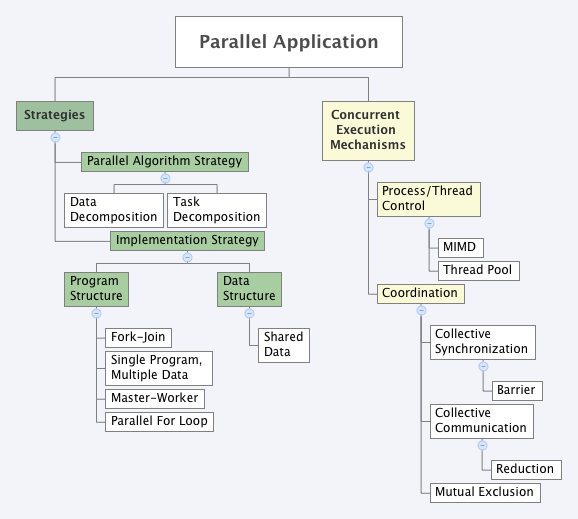
\includegraphics{OMP_Patterns.png}

Most programs you will write will include patterns for an Algorithm Strategy (both data decomposition and task decomposition), some of the Implementation Strategies (if not all), and some of the Coordination Mechanisms.  The patternlets show simple examples that you can use as a guide.  In OpenMP, most programs use various shared data in memory as their data structure implementation strategy. The Process/Thread Control Mechanism patterns are built in to any OpenMP program. Multiple Instruction, Multiple Data (MIMD) is built in because forked threads operate independently on different data. Likewise, pools of threads are part of every compiled OpenMP threaded program.



\renewcommand{\indexname}{Index}
\printindex
\end{document}
